% Распараллеливание.
\newpage
\section*{Глава 4. Распараллеливание вычислений с \mbox{передачей} сообщений и на общей памяти} % выключить номер главы
\addcontentsline{toc}{section}{Глава 4. Распараллеливание вычислений с передачей сообщений и на общей памяти} % но добавить ее в оглавление
\addtocounter{section}{1}                                                    % а теперь и счетчик продвинуть
\setcounter{subsection}{0}
\setcounter{figure}{0}
\setcounter{equation}{0}
\setcounter{table}{0}
\setcounter{theorem}{0}
\setcounter{lemma}{0}
\setcounter{definition}{0}

Эта глава посвящена задаче разработки методов повышения производительности параллельных вычислений на поверхностных и объемных расчетных сетках в моделях распараллеливания с передачей сообщений и на общей памяти.

Для решения крупных расчетных задач необходимо использование современных высокопроизводительных вычислительных систем.
Такие системы, как правило, состоят из множества отдельных вычислительных узлов, соединенных между собой каналами связи.
Таким образом, для решения задачи на высокопроизводительной вычислительной системе необходимо сначала разделить ее данные на отдельные подобласти, распределить эти данные по узлам вычислительной системы и организовать обмен сообщениями для учета взаимодействия подобластей \cite{GOST57700HPC}.
Подобласти данных решаемой задачи будем называть доменами, или партициями.
Использование вычислительных систем с большим количеством вычислительных узлов и запущенных на них вычислительных процессов продиктовано стремлением сократить время выполнения расчетов.

%---------------------------------------------------------------------------------------------------
% 4.1 - показатели распараллеливания с передачей сообщений

% Показатели эффективности декомпозиции сетки.
\subsection{Показатели распараллеливания в модели с \mbox{передачей} сообщений}

Основным показателем качества организации высокопроизводительных вычислений является ускорение расчетов исполнения при увеличении количества задействованных вычислительных узлов и запущенных на них вычислительных процессов.

\begin{definition}
Ускорением выполнения задачи в модели распараллеливания с передачей сообщений при использовании $k$ вычислительных процессов будем называть величину $s_{msg}(k) = \frac{T_1}{T_k}$, где $T_i$ -- время выполнения задачи с использованием $i$ вычислительных процессов. 
\end{definition}

В случае идеального сильного масштабирования вычислений $s_{msg}(k) = k$, то есть при увеличении количества процессов в $x$ раз при решении одной и той же расчетной задачи время выполнения этой задачи сокращается также в $x$ раз (в этом случае будем говорить, что наблюдается линейное ускорение вычислений).
Наряду с ускорением выполнения задачи при распараллеливании будем использовать характеристику эффективности распараллеливания.

\begin{definition}
Эффективностью распараллеливания при выполнении задачи в модели с передачей сообщений при использлвании $k$ вычислительных процессов будем называть величину $e_{msg}(k) = \frac{s_{msg}(k)}{k}$.
\end{definition}

Для идеального сильного масштабирования вычислений $e_{msg}(k) = 1$.
В дальнейшем будем использовать показатели $s_{msg}$ и $e_{msg}$ для оценки распараллеливания вычислений в модели с обменом сообщениями.

Высокопроизводительные вычисления, выполняющиеся на расчетных сетках, как правило, состоят из большого количества отдельных итераций по времени, на каждой из которых обрабатываются все ячейки сетки, а между итерациями подобласти расчетной задачи обмениваются данными расчетных ячеек, находящихся вблизи общих границ.
Сначала рассмотрим одну итерацию расчетов без учета информационных обменов.
Рассмотрим расчетную сетку, содержащую $n$ ячеек, и которую требуется декомпозировать на $k$ подобластей для обработки в $k$ вычислительных процессах (с номерами от $0$ до $k - 1$).
Все ячейки расчетной сетки могут обрабатываться параллельно.
Будем считать, что все ячейки являются одинаковыми с точки зрения времени их обработки.
Если разбить расчетную сетку на $k$ доменов с одинаковым количеством ячеек и обрабатывать каждый домен в отдельном процессе, то обработка каждого домена на одной итерации будет занимать одно и то же время.
Так как обработка всех доменов будет производиться параллельно, то это время и будет временем, затрачиваемым на одну итерацию обработки всех ячеек сетки.
Если распределение ячеек сетки по доменам будет неравномерным, то время выполнения одной итерации расчетов будет определяться самым крупным доменом (так как время его обработки будет максимальным).
Таким образом, в качестве показателя качества декомпозиции сетки можно принять максимальное абсолютное отклонение размера домена от теоретически возможного среднего значения
\begin{equation}
	D = \max_{0 \le i < k}{ \left( n_i - \frac{n}{k} \right) },
\end{equation}
где $n_i$ – количество ячеек в $i$-ом домене.
В идеальном случае равномерного распределения ячеек по доменам показатель $D$ становится равным нулю.
В худшем случае все ячейки распределяются в один домен, и $D = n \left( 1 - \frac{1}{k} \right)$.

Так как абсолютный показатель не слишком удобен для сравнения разных алгоритмов декомпозиции на разных сетках, то дополнительно будем использовать показатель, который характеризует долю накладных расходов неравномерного распределения ячеек по доменам по отношении к идеальному распределению, а именно
\begin{equation}
	D^{*} = \frac{D}{n / k}.
\end{equation}

Значение $D^{*}$ изменяется в диапазоне $[0, k - 1]$, где $D^{*} = 0$ означает идеальное распределение ячеек по доменам, а $D^{*} = k - 1$ соответствует наихудшему случаю, когда все ячейки отнесены к одному домену.
Также будем использовать величину $D^{\%} = D^{*} \cdot 100\%$ для возможности указания значения показателя в процентах.

\begin{definition}
Показатели $D$, $D^{*}$, $D^{\%}$ будем называть показателями неравномености декомпозиции расчетной сетки.
\end{definition} 

После завершения итерации расчетов требуется произвести информационные обмены данными на границах доменов.
Так как мы считаем, что каждый домен обрабатывается в своем процессе, то информационный обмен происходит с использованием механизмов межпроцессного взаимодействия (например, с использованием MPI).
Таким образом, для каждой пары доменов, имеющих общую границу необходимо организовывать межпроцессный обмен.
Все такие обмены могут происходить одновременно, и общее затрачиваемое на них время определяется длиной максимальной общей границы между доменами.
Для учета информационных обменов рассмотрим дуальный граф расчетной сетки $G = (V, E)$, вершинами которого являются ячейки сетки.
Две вершины в дуальном графе соединены ребром, если две соответствующие ячейки являются соседними (имеют общую грань).
Для каждого ребра $e \in E$ дуального графа под $e_a$ и $e_b$ будем понимать инцидентные ему вершины.
Тогда в качестве второй характеристики качества декомпозиции будем использовать величину наиболее протяженной границы между парой доменов, или
\begin{equation}
L_{ij} = \left| \{ e \in E: \{ d(e_a), d(e_b) \} = \{ i, j \} \} \right|, \ L = \max_{0 \le i < j < k}{L_{ij}},
\end{equation}
где $d(v)$ -- домен, к которому относится вершина $v$.
В идеальном случае значение характеристики $L$ может быть сколь угодно малым, даже нулевым (в случае, если сетка представляет собой $k$ одинаковых по количеству ячеек несвязных областей).
В наихудшем случае случае $L = |E|$, если ячейки распределены в два домена в шахматном порядке, и каждое ребро относится к границе между этими двумя доменами.

Наряду с показателем $L$ используется нормированный показатель $L^{*}$, определяемый как
\begin{equation}
	L^{*} = \frac{L}{|E|},
\end{equation}
который изменяется в диапазоне $[0, 1]$ и принимает значение 0 в идельном случае, а 1 -- в наихудшем.
Также будем использовать показатель длины максимальной границы между доменами в процентах от общего количества ребер $L^{\%} = L^{*} \cdot 100\%$.

\begin{definition}
Показатели $L$, $L^{*}$, $L^{\%}$ будем называть показателями максимальной длины границы между доменами при декомпозиции сетки.
\end{definition}

В качестве дополнительной характеристики качества декомпозиции можно использовать суммарную длину границ между доменами
\begin{equation}
	I = \sum_{0 \le i < j < k}{L_{ij}} = |\{ e \in E : d(e_a) \ne d(e_b) \}|,
\end{equation}
что соответствует общему количеству пересылаемых данных в рамках межпроцессного обмена.

\begin{definition}
Междоменным, или кроссдоменным ребром $e \in E$ дуального графа будем называть ребро, инцидентные вершины которого относятся к разным доменам, то есть $d(e_a) \ne d(e_b)$.
\end{definition}

Так как домены граничат между собой по ребрам дуального графа, то суммарная длина всех границ между доменами представляет собой просто количество всех междоменных ребер.
Наряду с показателем $I$ будем использовать долю междоменных ребер среди общего количества ребер сетки
\begin{equation}
	I^{*} = \frac{I}{|E|}.
\end{equation}

Показатель $I^{*}$ также является нормированным, он изменяется в диапазоне $[0, 1]$ и принимает значение 0 в идеальном случае и 1 -- в наихудшем.
Также будем использовать показатель количества междоменных ребер в процентах от общего количества ребер $I^{\%} = I^{*} \cdot 100\%$.

\begin{definition}
Показатели $I$, $I^{*}$, $I^{\%}$ будем называть показателями суммарной длины границ между доменами при декомпозиции расчетной сетки.
\end{definition}

%---------------------------------------------------------------------------------------------------
% 4.2 - распределение вычислительной нагрузки с дроблением

\subsection{Распределение вычислительной нагрузки между \mbox{процессами} с дроблением блоков расчетной сетки}

\subsubsection{Блочно-структурированная расчетная сетка и организация межпроцессных обменов}\label{sec:par_block_struct_mesh}

Одним из распространенных типов расчетных сеток является блочно-структурированная сетка, состоящая из нескольких блоков, некоторые из которых имеют общие границы.
Такая структура позволяет выполнять вычисления для различных блоков независимо друг от друга, обмениваясь общими данными на границах.
Для эффективного проведения вычислений на блочно-структурированных сетках важную роль имеет реализация сетки в виде внутреннего представления и организация механизма межпроцессного обмена данными между соседними блоками сетки \cite{Rybakov2017Mesh}.

Будем рассматривать объемные блочно-структурированные сетки, состоящие из отдельных блоков, каждый из которых представляет собой упорядоченный трехмерный массив ячеек, имеющих форму кубоида.
Упорядоченность размещения ячеек обеспечивает быстрый доступ к ячейками по индексам и снижает требования к объему памяти, однако строить блочно-структурированные сетки гораздо сложнее, чем неструктурированные.

Блоки блочно-структурированной сетки могут иметь сложную форму.
Для доступа к отдельным ячейкам блока вводятся три индекса, связанные с криволинейной системой координат блока.
Система координат задается тремя линиями координат $(I, J, K)$, каждая из которых связывает пары противоположных граней блока.
Для наглядности будем изображать блоки сетки в виде прямоугольных параллелепипедов, как показано на рис.~\ref{fig:text_2_block_block} слева.

\begin{figure}[ht]
\centering
\begin{tabular}{ll}
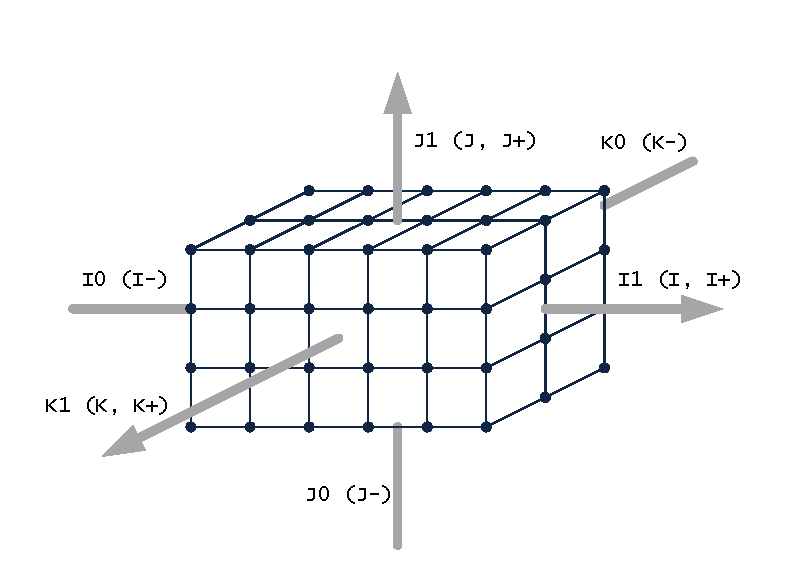
\includegraphics[width=0.45\textwidth]{fig/par_1-block.pdf}
&
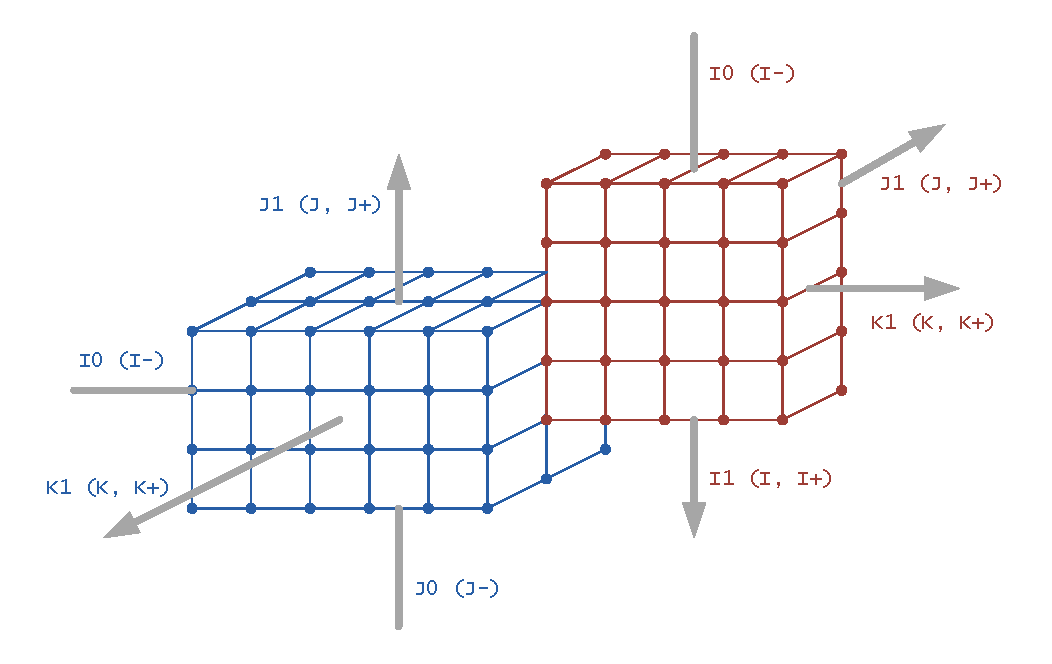
\includegraphics[width=0.45\textwidth]{fig/par_2-block-block.pdf}
\end{tabular}
\singlespacing
\captionstyle{center}\caption{Блок сетки (слева) и касание блоков (справа).}
\label{fig:text_2_block_block}
\end{figure}

Блоки могут граничить между собой.

\begin{definition}
Интерфесом будем называть описание области границы одного блока, по которой он касается другого блока расчетной сетки.
\end{definition}

Один интерфейс описывает соприкосновение двух блоков прямоугольными подобластями своих граней.
При этом системы координат двух соседних блоков не обязаны согласовываться между собой.
Пример касания двух блоков приведен на рис.~\ref{fig:text_2_block_block} справа.

Выполнение расчетов на сетке носит итерационный по времени характер.
Для каждой итерации по времени выполняется пересчет расчетных данных ячеек согласно той или иной вычислительной схеме.
Во время обработки одной ячейки возникает потребность обращаться за данными к другим ячейкам, находящимся рядом с рассматриваемой.

\begin{definition}
Совокупность ячеек расчетной сетки, данные которых используются при обработке конкретной ячейки, называют вычислительным шаблоном, или вычислительной молекулой, или вычислительной окрестностью этой ячейки.
\end{definition}

\begin{figure}[ht]
\centering
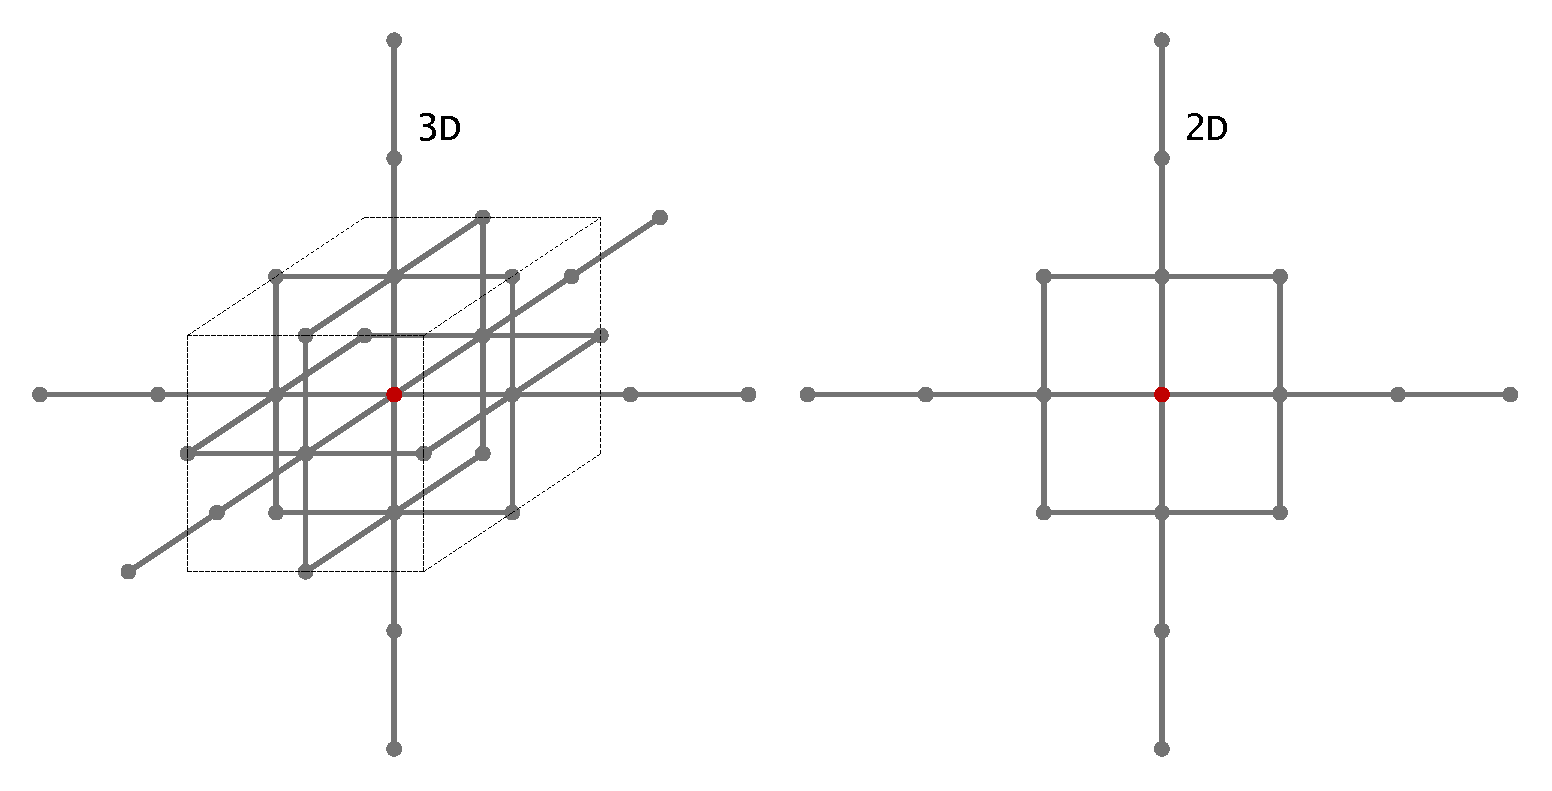
\includegraphics[width=0.8\textwidth]{fig/par_3-cell-delta.pdf}
\singlespacing
\captionstyle{center}\caption{Примеры вычислительных окрестностей ячеек сетки.}
\label{fig:text_2_block_cell_delta}
\end{figure}

На рис.~\ref{fig:text_2_block_cell_delta} показаны примеры вычислительных окрестностей ячейки.
В дальнейшем для большей наглядности будем изображать блоки в двумерном виде (с системой координат $IJ$).
Во время произведения расчетов различные блоки сетки обрабатываются независимо друг от друга.
При этом для некоторых ячеек обрабатываемого блока их вычислительные окрестности выходят за границу блока и затрагивают соседние блоки.
Для эффективного счета необходимо обеспечить функционал обмена данными между блоками.
Если два соседних блока обрабатываются в разных вычислительных процессах, то для обмена данными нужно использовать передачу сообщений.
Приведем классификацию ячеек внутри блока сетки (см. рис.~\ref{fig:text_2_block_block_cells}) слева.

\begin{figure}[ht]
\centering
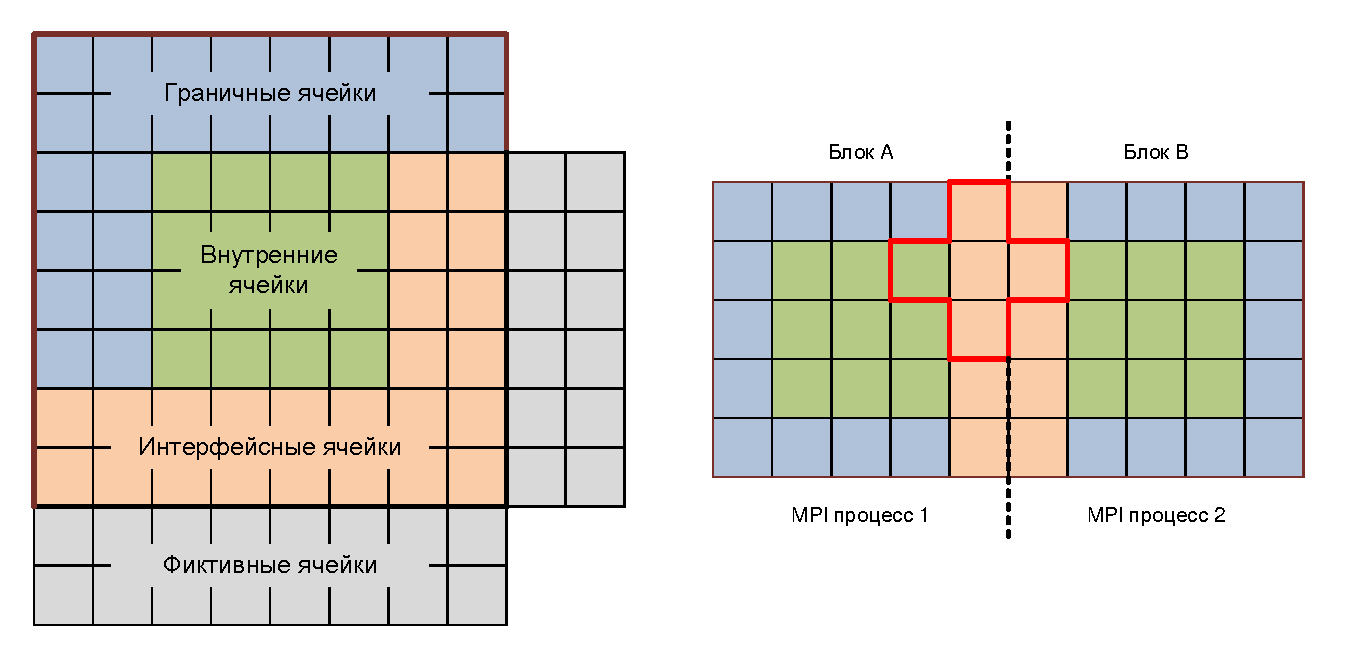
\includegraphics[width=0.8\textwidth]{fig/par_4-block-cells.pdf}
\singlespacing
\captionstyle{center}\caption{Ячейки разных типов.}
\label{fig:text_2_block_block_cells}
\end{figure}

\begin{definition}
Внутренними ячейками (Inner Cells) будем называть те ячейки блока, вся вычислительная окрестность которых лежит внутри того же блока.
\end{definition}

\begin{definition}
Ячейки, не являющиеся внутренними ячейками блока, будем называть граничными ячейками (Border Cells).
\end{definition}

\begin{definition}
Если окрестность ячейки частично накрывает один из соседних блоков, то такую ячейку будем относить к интерфейсным ячейкам (Interface Cells), так как ее окрестность пересекает интерфейс блока.
\end{definition}

\begin{definition}
Если окрестность ячейки частично накрывает некоторый блок, который обрабатывается в другом вычислительном процессе, то будем относить ее к ячейкам MPI\label{abbr:mpi-1} обмена (MPI Cells), так как для получения данных этой окрестности нужно использовать средства межпроцессного обмена (см. рис.~\ref{fig:text_2_block_block_cells} справа).
\end{definition}

При обработке ячеек MPI обмена мы должны обращаться за данными к другому процессу.
Если делать это только по мере необходимости, то придется совершать большое количество обменов, что негативно скажется на производительности.
Поэтому для повышения быстродействия вместо этого для блока заводится специальный слой внешних ячеек, куда копируются все необходимые данные из соседних процессов, которые могут понадобиться при обработке блока.
Такие ячейки будем называть фиктивными.

\begin{definition}
Фиктивными ячейками блока будем называть дополнительно созданные для этого блока ячейки, которые содержат скопированные из соседних блоков данные, необходимые для выполнения вычислений в рассматриваемом блоке.
Множество фиктивных ячеек блока также будем называть его теневым слоем.
\end{definition}

Ширина теневого слоя блока определяется размером вычислительного шаблона обработки ячейки.
Объединение всех ячеек блока с множеством фиктивных ячеек является замкнутой структурой, которая более не требует для своей обработки обращений к другим вычислительным процессам на одной итерации выполнения расчетов.

Опишем основные объекты, используемые для организации работы с блочно-структурированной сеткой и проведения вычисления на ней \cite{CertRybakov2020PrepStruct}.

Основным объектом блочно-структурированной расчетной сетки является блок (Block) (см. рис.~\ref{fig:text_2_block_block_and_coords}). 
Блок состоит из трехмерного массива ячеек размера $a \times b \times c$ ($a$, $b$, $c$ -- размеры вдоль измерений $I$, $J$ и $K$ соответственно).
Каждая ячейка содержит набор физических величин, ассоциированных с центром ячейки, и другие вспомогательные данные.
Также блок содержит данные о всех вершинах своих ячеек, эти данные хранятся в трехмерном массиве размера $(a + 1) \times (b + 1) \times (c + 1)$.
Для определения геометрии блока необходимо задать его линейные размеры и координаты всех его узлов.

\begin{figure}[ht]
\centering
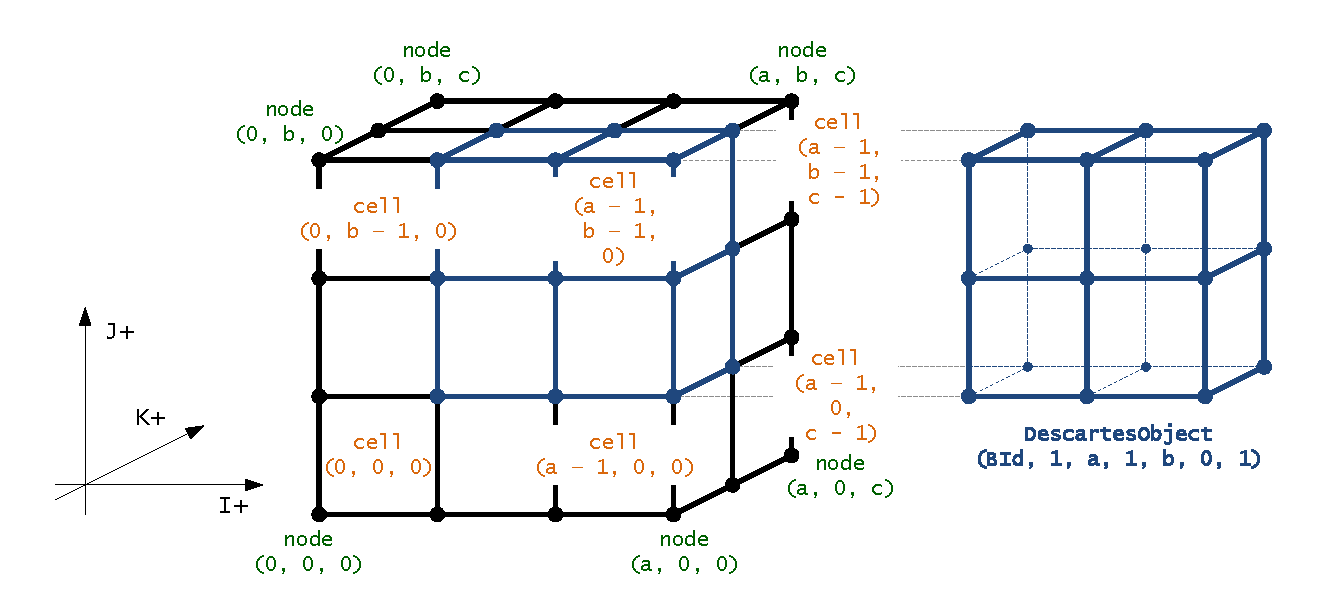
\includegraphics[width=0.7\textwidth]{fig/par_block_coords.pdf}
\singlespacing
\captionstyle{center}\caption{Блок сетки и координаты его узлов.}
\label{fig:text_2_block_block_and_coords}
\end{figure}

\begin{figure}[ht]
\centering
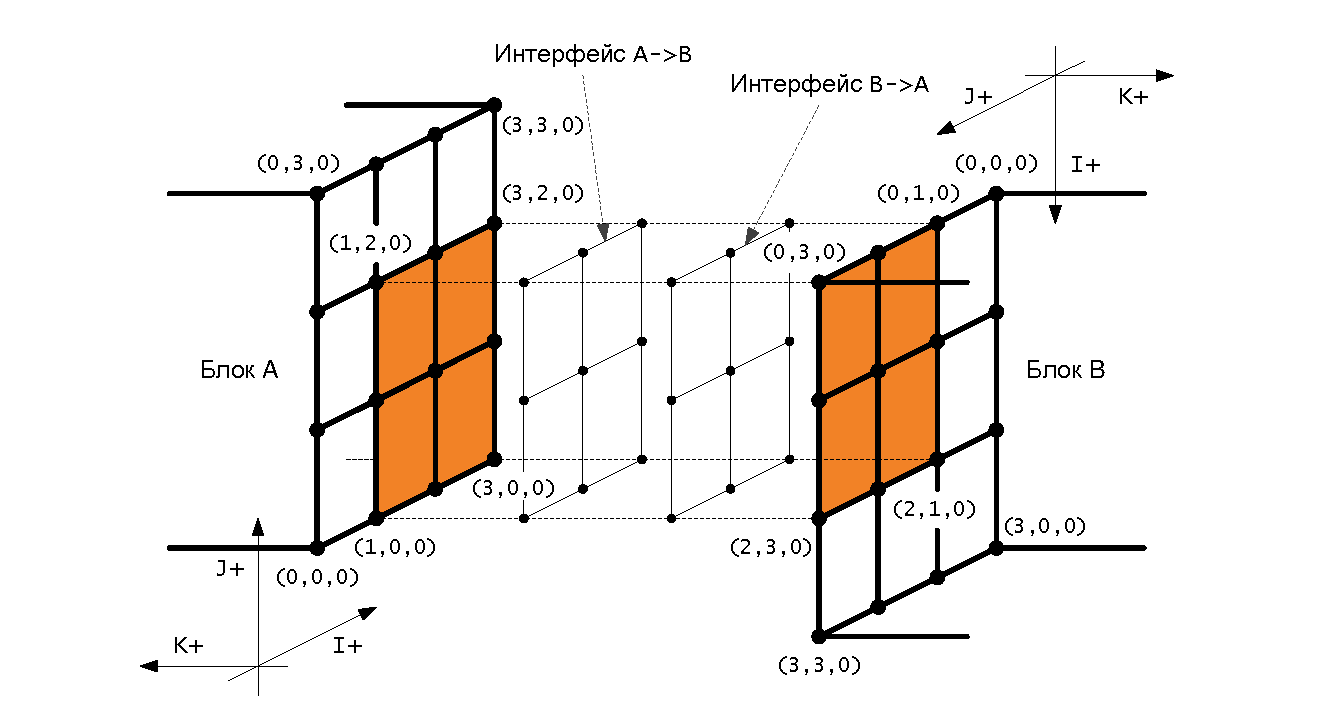
\includegraphics[width=0.8\textwidth]{fig/par_7-iface.pdf}
\singlespacing
\captionstyle{center}\caption{Структура интерфейса касания блоков.}
\label{fig:text_2_block_iface}
\end{figure}

Объектом, описывающим соприкосновение двух соседних блоков, является интерфейс (Iface) (см. рис.~\ref{fig:text_2_block_iface}).
Интерфейс является однонаправленным, он сообщает, что у рассматриваемого блока конкретная прямоугольная часть границы соприкасается с другим блоком.
Чтобы определить с какой частью другого блока граничит рассматриваемый блок, нужно рассмотреть смежный ему интерфейс.
Таким образом полная информация о касании двух соседних блоков описывается парой смежных интерфейсов.
Интерфейс описывается в системе координат того блока, к которому он относится.
Координаты задают размер области соприкосновения по всем трем направлениям.
В приведенном на рис.~\ref{fig:text_2_block_iface} примере касания двух блоков два смежных интерфейса, описывающих касание блоков $A$ и $B$, задаются следующим образом: $A(1, 3, 0, 2, 0, 0) \rightarrow B$, $B(0, 2, 1, 3, 0, 0) \rightarrow A$.

На границе блока кроме другого блока может находиться граница расчетной области.
В этом случае на границе блока необходимо задать граничные условия (BCond).
Граничные условия задаются аналогично интерфейсу (с помощью системы координат блока), однако вместо соседнего блока подается ссылка на описатель граничных условий.
Таким образом, и интерфейс и граничное условие являются частным случаем границы блока (Border).

В процессе вычислений необходимо иметь возможность быстро узнать для конкретной граничной ячейки, какого типа граница ей соответствует и быстро найти соответствующий интерфейс или граничное условие.
Для этой цели служат грани блока (Facet).
Каждый блок имеет 6 граней (для каждого из направлений $I^{-}$, $I^{+}$, $J^{-}$, $J^{+}$, $K^{-}$, $K^{+}$).
Каждая грань является двумерным массивом, содержащим для каждой ячейки, граничащей с гранью, ссылку на интерфейс или на граничное условие (см. рис.~\ref{fig:text_2_block_facet}).

\begin{figure}[ht]
\centering
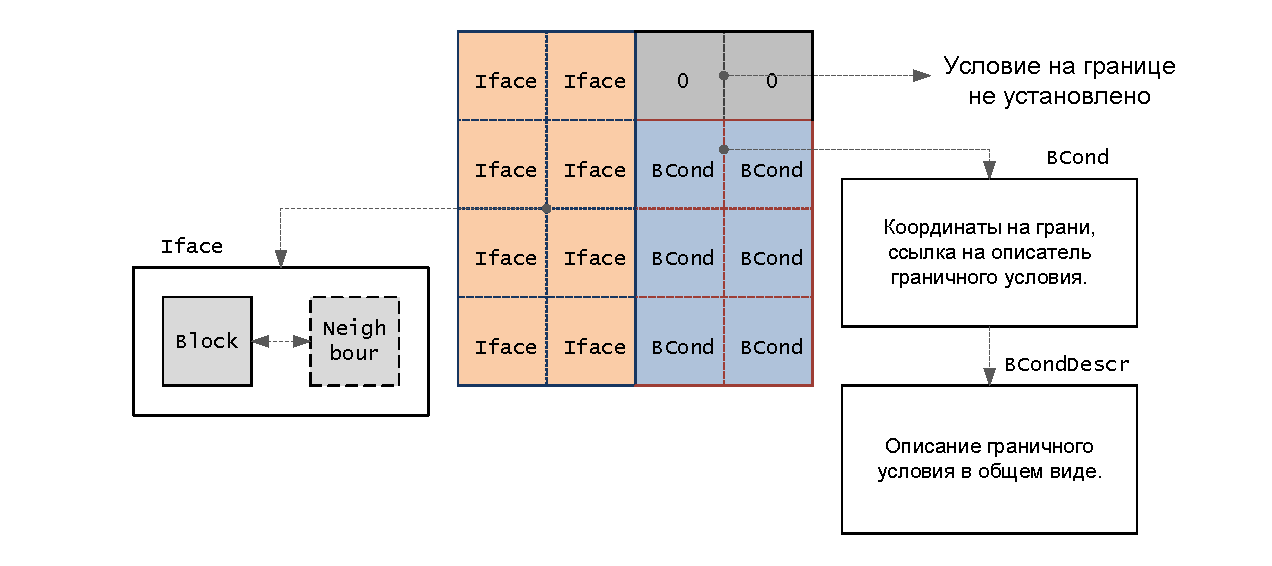
\includegraphics[width=0.8\textwidth]{fig/par_8-facet.pdf}
\singlespacing
\captionstyle{center}\caption{Структура грани блока.}
\label{fig:text_2_block_facet}
\end{figure}

Для описания начальных условий используется область блока (Scope), которая реализована аналогично граничным условиям, но является трехмерным объектом.

Таким образом, все основные объекты расчетной сетки являются двумерными или трехмерными декартовыми объектами, то есть такими объектами, чья геометрия задается двумерными или трехмерными массивами узлов блоков сетки.
Также заметим, что граничные условия и области являются именованными объектами, так как им присваиваются имена для определения механизмов задания граничных и начальных условий расчета.
Исходя из этого, получаем следующую иерархию классов, реализующих расчетную сетку (см. рис.~\ref{fig:text_2_block_hierarchy}).

\begin{figure}[ht]
\centering
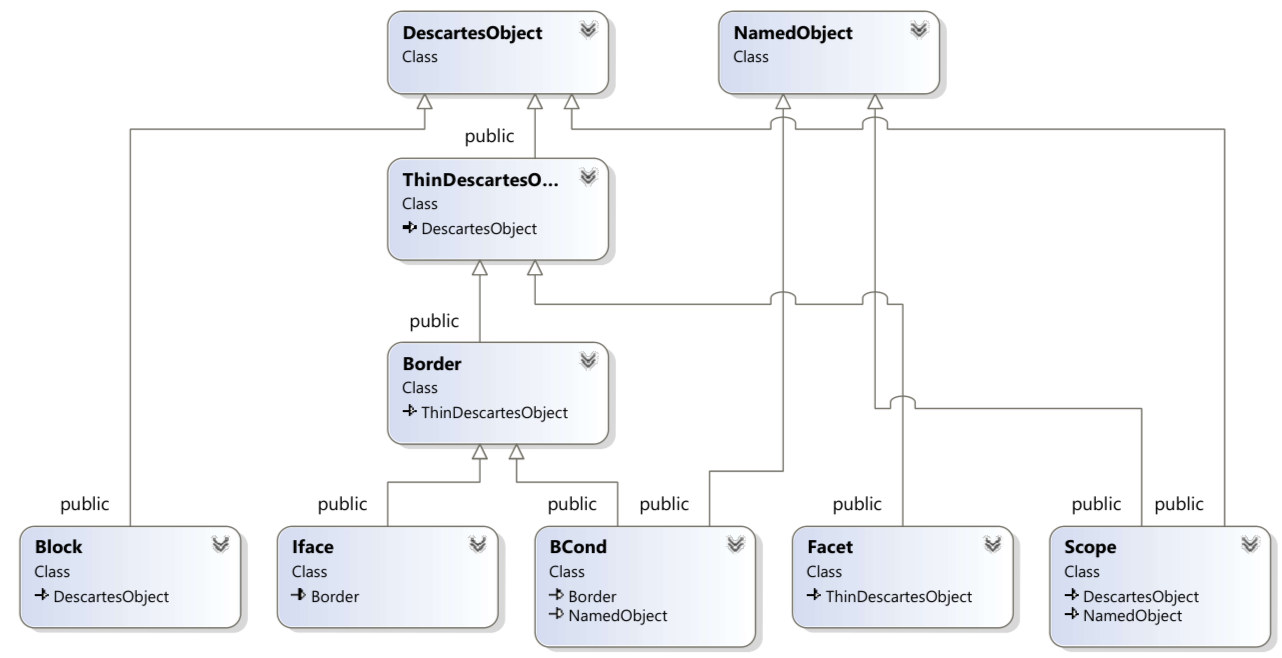
\includegraphics[width=0.8\textwidth]{fig/par_9-hierarchy.png}
\singlespacing
\captionstyle{center}\caption{Иерархия объектов внутреннего представления сетки.}
\label{fig:text_2_block_hierarchy}
\end{figure}

Рассмотрим механизм обмена данными между блоками сетки.
Если два соседние блока, между которыми должен быть осуществлен обмен данными, обрабатываются в разных процессах при выполнении расчетов на суперкомпьютере, то обмен данными может быть осуществлен с помощью обмена сообщениями с использованием MPI\label{abbr:mpi-2}.
Каждый блок должен отправить своим соседям данные, находящиеся в его интерфейсных ячейках, и получить данные, которые соответствуют ячейкам его теневого слоя.

Логика обменов устроена следующим образом.
Так как пара смежных интерфейсов определяет факт касания двух блоков, между которыми должен произойти обмен, то на каждом из этих интерфейсов заводится буфер для данных обмена, после чего происходит обмен данными буферами (см. рис.~\ref{fig:text_2_block_data_exchange}).
Обмены данными происходят одновременно по всем интерфейсам сетки с помощью асинхронных функций
\texttt{MPI\_Isend}, \texttt{MPI\_Irecv}.
Рассмотрим механизм обмена данными между соседними блоками, находящимися в разных процессах, более подробно.

\begin{figure}[ht]
\centering
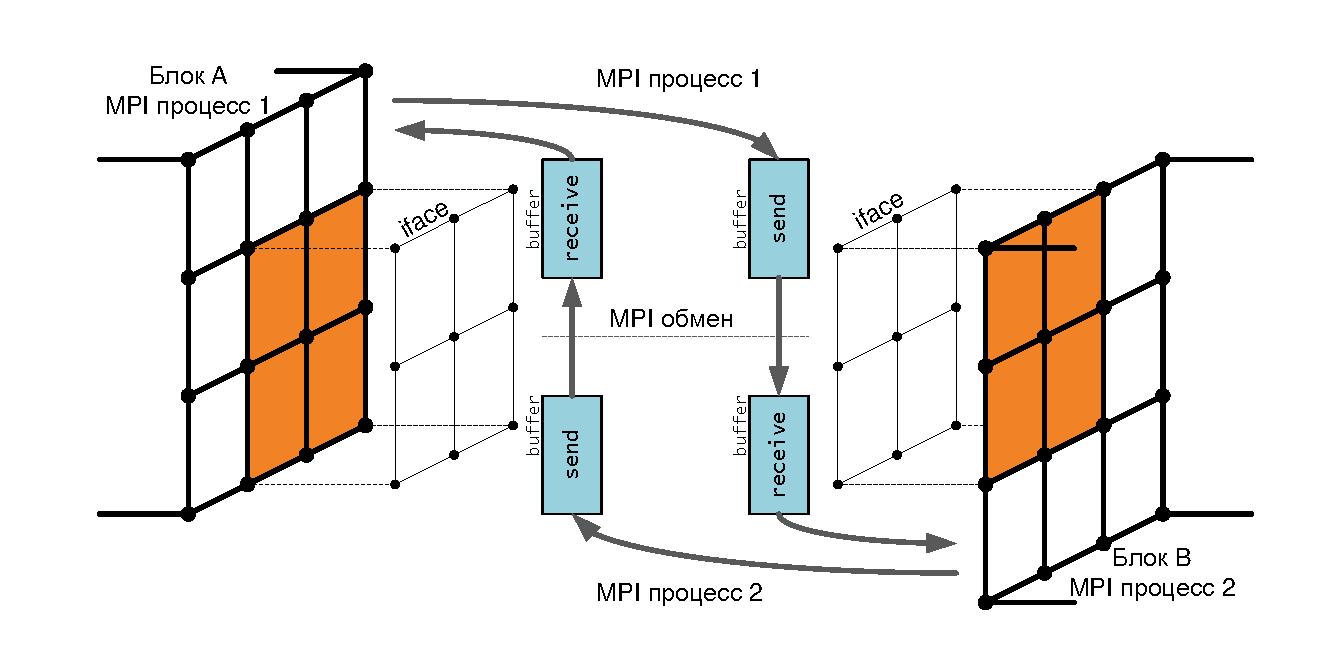
\includegraphics[width=0.8\textwidth]{fig/par_10-data-exchange.pdf}
\singlespacing
\captionstyle{center}\caption{Обмен данными между блоками сетки.}
\label{fig:text_2_block_data_exchange}
\end{figure}

Пусть Блок $A$ обрабатывается в процессе 1, а блок $B$ -- в процессе 2, как показано на рис.~\ref{fig:text_2_block_data_exchange}.
Каждый из двух смежных интерфейсов, описывающих касание этих двух блоков имеет свой буфер обмена данными.
Так как в процессе 1 активным является блок $A$, то буфер его интерфейса работает на прием данных, а буфер интерфейса со стороны блока $B$ -- на отправку (данных блока $A$).
В процессе 2 все происходит ровно наоборот: активным является блок $B$, буфер интерфейса блока $A$ работает на отправку данных блока $B$, буфер интерфейса со стороны блока $B$ работает на прием данных.
Для всех интерфейсов происходит асинхронный запуск всех вызовов функций обмена, после чего происходит ожидание завершения всех операций.
После этого каждый блок может извлечь данные из буфера интерфейса, в котором он является активным, и поместить эти данные в свою теневую зону, после чего начинается следующая итерация расчетов.

\begin{figure}[ht]
\centering
\begin{tabular}{l}
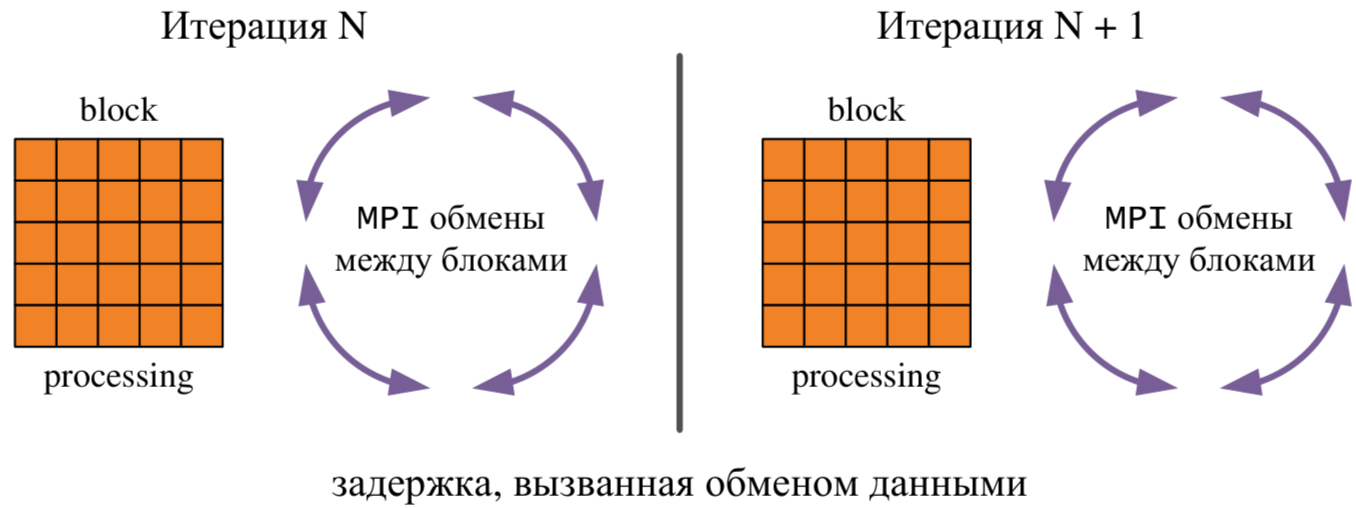
\includegraphics[width=0.5\textwidth]{fig/par_11-mpi1.png}
\\
\\
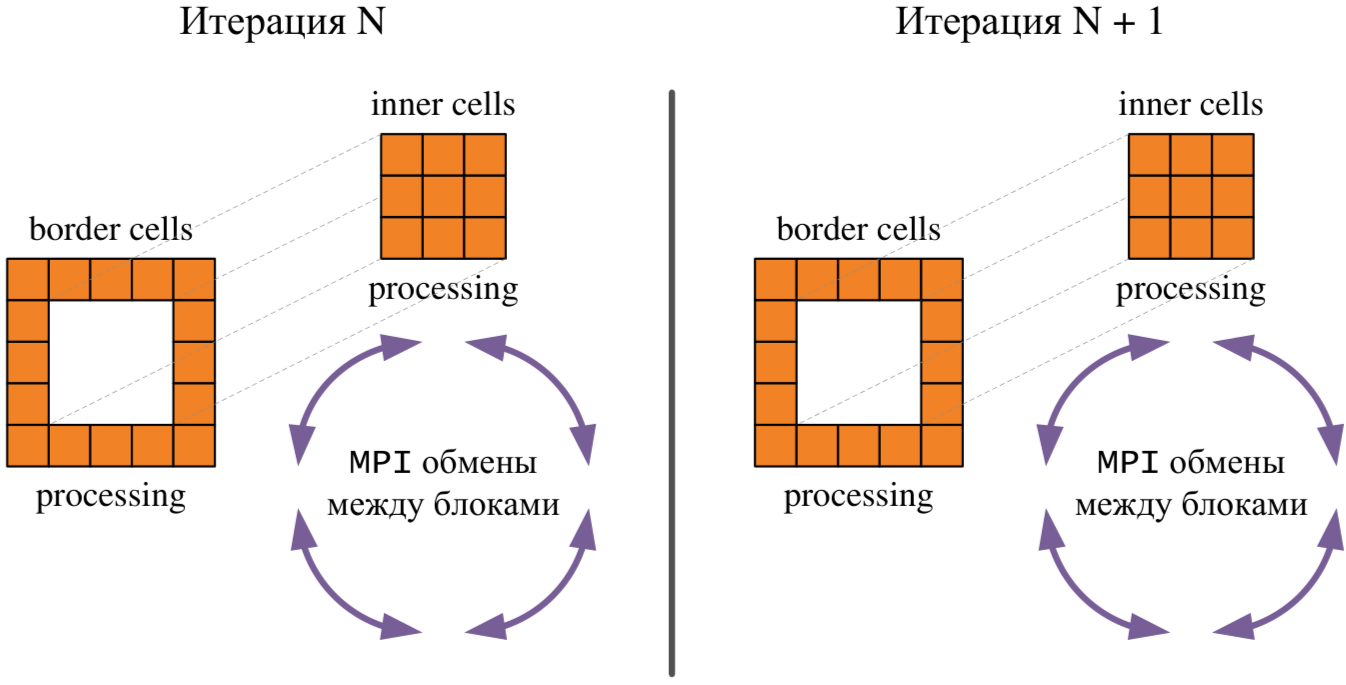
\includegraphics[width=0.5\textwidth]{fig/par_12-mpi2.png}
\end{tabular}
\singlespacing
\captionstyle{center}\caption{Задержки, вызванные MPI\label{abbr:mpi-3} обменами и избавление от них.}
\label{fig:text_2_block_mpi1}
\end{figure}

После проведения каждой итерации счета задачи необходимо выполнять обмен данными, чтобы состояния граничных ячеек блоков были актуальными.
При этом начинать обсчет следующей итерации нельзя до завершения всех обменов.
Это может привести к возникновению задержек (см. рис.~\ref{fig:text_2_block_mpi1}, сверху).
Чтобы избежать такого рода потери вычислительного времени можно разделить обработку ячеек блока на отдельную обработку всех внутренних ячеек и обработку граничных ячеек.
Сначала нужно произвести обработку всех граничных ячеек блока, затем инициировать асинхронные обмены данными (в которых участвуют только граничные ячейки), а затем сразу начать обработку внутренних ячеек, для которых получение данных фиктивных ячеек не требуется.
Такой подход позволяет скрыть издержки на коммуникацию за полезными вычислениями (см. рис.~\ref{fig:text_2_block_mpi1}, снизу).

Особенности структуры и реализации внутреннего представления блочно-структурированной сетки имеют большое значение для выполнения расчетов.
Выбор модели сетки, способы расположения данных в памяти и другие факторы напрямую влияют на эффективность выполнения программы.
Важную роль в скорости выполнения расчетов играет реализация механизма обмена данными в случае запуска вычисления на суперкомпьютере.
Так как обмен данными должен происходить на каждой итерации вычислений, то это является узким местом для повышения эффективности расчетов.

% Распределение вычислительной нагрузки между узлами гетерогенного вычислительного кластера.
\subsubsection{Распределение вычислительной нагрузки между узлами \mbox{вычислительного} кластера}\label{sec:text_2_getero}

Рассмотрим фиксированную декомпозированную расчетную задачу.
Это могут быть вычисления, выполняемые на блочно-структурированной расчетной сетке, либо на неструктурированной сетке, разбитой на домены.
При распределении частей расчетной задачи между вычислителями суперкомпьютерного кластера для уменьшения времени выполнения задачи необходимо учитывать характеристики самого кластера, к которым относится производительность вычислителей и скорость обмена данными между ними.
В этом разделе приводится постановка задачи распределения вычислительной нагрузки на вычислительном кластере с учетом топологии расчетной задачи и характеристик кластера \cite{Rybakov2018Distr,Rybakov2017Part}.

\begin{definition}
Графом вычислительного кластера назовем граф $H = (V_H, E_H)$.
Узлы этого графа соответствуют отдельным вычислителям кластера (одному процессору или сопроцессору), а ребра -- логическим соединениям между вычислителями (то есть возможностью обмена данными).
\end{definition}

Так как между любыми двумя вычислителями возможен обмен данными, то граф $H$ является полным (и даже является псевдографом, так как содержит петли).
Введем на графе $H$ две весовые функции.
Первая функция $f: V_H \rightarrow \mathbb{R}_{> 0}$ каждому узлу графа ставит в соответствие скорость работы соответствующего вычислителя, то есть количество расчетных данных, которые могут быть обработаны на нем за одну условную единицу времени.
Вторая функция $l: E_H \rightarrow \mathbb{R}_{> 0}$ несет смысл скорости обмена данными между вычислителями, она показывает количество данных, которые могут быть переданы между соответствующими вычислителями за одну условную единицу времени.

\begin{definition}
Графом расчетной задачи назовем граф $G = (V_G, E_G)$, который отражает особенности декомпозиции расчетной области (это может быть граф блочно-структурированной расчетной сетки или граф доменов неструктурированной сетки).
Узлы этого графа соответствуют подобластям данных задачи, каждое из которых обрабатывается одним вычислителем.
Ребра графа соответствуют потокам данных между разными частями задачи.
\end{definition}

На графе $G$ также вводятся две весовые функции.
Первая функция $w: V_G \rightarrow \mathbb{R}_{> 0}$ имеет значение объема вычислительных данных, обрабатываемых в соответствующей части задачи.
Вторая функция $i: E_G \rightarrow \mathbb{R}_{> 0}$ отражает объем данных, пересылаемых между частями задачи при межпроцессном обмене.
Значения всех четырех функций $f$, $l$, $w$, $i$ измеряются в одних и тех же единицах (это могут быть ячейки расчетной сетки, количество байтов или вещественных значений).
Однако $w$ и $i$ имеют смысл объема вычислений и пересылок, тогда как функции $f$ и $l$ относятся к фиксированной единице времени, то есть имеют смысл скорости обработки и пересылки данных.

Расчет задачи состоит из двух чередующихся фаз: проведение итерации расчета и выполнение межпроцессных обменов данными.
Требуется таким образом распределить задачу между вычислителями кластера, чтобы суммарное время одной итерации расчета и одной итерации межпроцессных обменов было минимально.
Распределение задачи между вычислителями кластера определяется функцией $\gamma: V_G \rightarrow V_H$.

Время выполнения одной итерации вычислений определяется по самому загруженному вычислителю:
\begin{equation}
	t_1^{max} = \max_{v_H \in V_H}{ \left\{ \frac{1}{f(v_H)} \sum_{\substack{v_G \in V_G \\ \gamma(v_G) = v_H}}{w(v_G)} \right\} }.
\end{equation}

Аналогично время выполнения одной итерации межпроцессных обменов определяется по самому загруженному каналу обмена:
\begin{equation}
	t_2^{max} = \max_{e_H \in E_H}{ \left\{ \frac{1}{l(e_H)} \sum_{\substack{e_G = (u_G, v_G) \in E_G \\ (\gamma(u_G), \gamma(v_G)) = e_H}}{i(e_G)} \right\} }.
\end{equation}

Таким образом, задача поиска оптимального распределения задачи по вычислителям кластера сводится к поиску функции $\gamma$, минимизирующей значение функционала $t^{max}(\gamma) = t_1^{max}(\gamma) + t_2^{max}(\gamma)$.

Можно рассматривать частные случае задачи распределения вычислительной нагрузки.
Для вычислительных задач с малой долей мепроцессных обменов можно ограничиться минимизацией функционала $t^{max}(\gamma) = t_1^{max}(\gamma)$.
Также можно рассматривать задачу распределения для гомогенного кластера, для которого функции $f$ и $l$ являются константами.
Минимизируемый функционал в этом случает принимает следующий вид:
\begin{equation}
	t^{max}(\gamma) =
		\frac{1}{f} \max_{v_H \in V_H}{ \left\{ \sum_{\substack{v_G \in V_G \\ \gamma(v_G) = v_H}}{w(v_G)} \right\} } + 
		\frac{1}{l} \max_{e_H \in E_H}{ \left\{ \sum_{\substack{e_G = (u_G, v_G) \in E_G \\ (\gamma(u_G), \gamma(v_G)) = e_H}}{i(e_G)} \right\} }.
\end{equation}

Далее будем рассматривать распределение вычислительной нагрузки между процессами гомогенного вычислительного кластера без учета характеристик каналов связи между вычислителями, то есть $t^{max}(\gamma) = t_1^{max}(\gamma)$ в применении к блочно-структурированным расчетным сеткам.

\newpage
\subsubsection{Распределение блоков по вычислительным процессам без дробления блоков}

Для распределения блоков расчетной сетки по вычислительным процессам рассмотрим следующую задачу разделения множества $m$ весов на $k$ подмножеств.
Пусть дано множество $X$ вещественных чисел $x_i \ge 0$ для $i \in M$, где $M = [0, m - 1]$.
Рассмотрим также множество индексов $j \in K$, где $K = [0, k - 1]$.
Будем говорить, что определено разбиение множества $X$ на $k$ подмножеств, если введена функция $\gamma: M \rightarrow K$.
Множество всех функций разбиения будем обозначать $\Gamma(M, K)$.
Веса результирующих подмножеств будем определять естественным образом для $j \in K$:
\begin{equation}
	X_j = \sum_{\substack{i \in M \\ \gamma(i) = j}}{x_i}.
\end{equation}

Требуется найти такую функцию разбиения $\gamma \in \Gamma(M, K)$, чтобы минимизировать наиболее тяжелое из результирующих подмножеств $X^{max} = \max_{j \in K}{X_j}$.

Задача может быть расширена на случай распределения вычислительной нагрузки между вычислителями суперкомпьютера с разной производительностью.
При этом формулировка задачи меняется только в части приведения всех процессов к одному показателю с помощью весовых коэффициентов.
Коэффициентом приведения $\kappa(j)$ для $j \in K$ назовем такую положительную функцию $\kappa: K \rightarrow \mathbb{R}_{>0}$, что время выполнения нагрузки $\kappa(j)$ на процессе $j$ не зависит от $j$.
Тогда в общем случае задача о разбиении множества $m$ весов на $k$ подмножеств с коэффициентами приведения $\kappa(j)$ для $j \in K$ формулируется следующим образом.
Требуется найти такую функцию разбиения $\gamma \in \Gamma(M, K)$, чтобы минимизировать наболее тяжелое из результирующих подмножеств с учетом коэффициентов приведения $\max_{j \in K}{ \frac{X_j}{\kappa(j)} }$.
Эта задача имеет практическое применение при распределении вычислительной нагрузки между вычислителями гетерогенного суперкомпьютера.
Далее будем рассматривать задачу без учета весовых коэффициентов $\kappa$.

Поставленная задача о рапределении множества $m$ весов на $k$ подмножеств при условии минимизации $X^{max}$ связана с большими вычислительными затратами.
В \cite{Romanovskii1977Extreme} можно найти описание алгоритма решения этой задачи (называемой задачей о куче камней), основанного на решении другой, так называемой $z$-задачи, которая формулируется следующим образом: определить, существует ли такое разбиение множества $m$ весов на $k$ подмножеств, для которого выполнено условие $X^{max} \le z$.
Используя $z$-задачу, исходную задачу о разбиении с минимизацией $X^{max}$ можно решить с помощью бинарного поиска.
Решение же $z$-задачи выполняется методом ветвей и границ с односторонним обходом дерева вариантов разбиения.
При решении $z$-выполняется попытка последовательно заполнить каждое из $k$ подмножеств весами, начиная с наибольшего, не превышая ограничения на вес подмножества $z$.
При этом в памяти постоянно хранится значения общего свободного места в результирующих подмножествах.
Если значение общего свободного места становится отрицательным, то последнее действие по назначению веса в подмножество отменяется и продолжается перебор по дереву вариантов.
Такой подход хоть существенно сокращает время работы алгоритма, однако не снижает его сложность и при больших значениях $m$ и $k$ неприменим.

С другой стороны, поставленная задача может быть решена приближенно с помощью жадного алгоритма.
Опишем последовательность действий жадного алгоритма.
Множество распределяемых весов будем хранить в виде массива, который перед началом работы алгоритма отсортируем по убыванию.
Далее в алгоритме будем последовательно обрабатывать все веса, начиная с наибольшего.
Каждый необработанный вес будем относить к наиболее легкому на текущий момент подмножеству весов.
Эта последовательность действий формализована как алгоритм~\ref{alg:par_greedy_simple}.

\begin{algo}\label{alg:par_greedy_simple}
Жадный алгоритм распределения множества весов по подмножествам.
\begin{algorithm}
\DontPrintSemicolon
\KwInput{$m$ -- количество распределяемых весов, $X = [x_0, x_1, \ldots, x_{m - 1}]$ -- массив распределяемых весов, $k$ -- количество результирующих подмножеств.}
\KwOutput{$[\gamma_0, \gamma_1, \ldots, \gamma_{m - 1}]$ -- массив, в котором элемент $\gamma_i$ содержит номер подмножества, к которому отнесен вес $x_i$.}
отсортировать массив $X$ по убыванию\;
$P \leftarrow \{ p : p.w = 0, p.i = i, \forall i \in [0, k - 1] \}$ -- множество, описывающее текущее состояние результирующих подмножеств, где $p.w$ -- вес подмножества, $p.i$ -- его номер, а сравнение подмножеств выполняется по весу\;
\For{$i \leftarrow 0$ \KwTo $(m - 1)$}
{
	$p \leftarrow P.min$\;
	$p.w \leftarrow p.w + x_i$\;	
	$\gamma_i = p.i$\;
}
\end{algorithm}
\end{algo}

Сложность алгоритма зависит от используемой реализации множества $P$.
Целесообразно реализовать множество $P$ с помощью упорядоченного по возрастанию множества пар (вес, индекс), тогда создание этого множества будет иметь сложность $O(k)$, поиск минимального элемента $O(1)$, а обновление веса $O(\log k)$.
С учетом затрат на сортировку массива распределяемых весов в результате получим сложность всего алгоритма $O(m (\log m + \log k) + k)$.
$\blacksquare$\\

Проведем анализ эффективности работы алгоритма~\ref{alg:par_greedy_simple}.
Для удобства без ограничения общности будем считать, что изначальное множество весов упорядочено по убыванию.

Определим остаточный член $r_i$ для $i \in M$ по следующей формуле:
\begin{equation}
	r_i = \max{\left( x_i - \frac{1}{k} \sum_{p = i}^{m}{x_p}, 0 \right)}.
\end{equation}

В приведенных обозначениях и предположениях верна следующая лемма:

\begin{lemma}\label{lem:text_2_withcut_lem}
При использовании жадного алгоритма разбиения множества $m$ весов на $k$ подмножеств отклонение наиболее тяжелого подмножества $X^{max}$ от среднего значения веса подмножеств $X^{avg} = \frac{1}{k} \sum_{j \in K}{X_j}$ не превышает максимальный остаточный член $r_i$, то есть
\begin{equation}
	X^{max} - X^{avg} \le \max_{i \in M}{r_i}.
\end{equation}
\end{lemma}
Пусть $X_q = X^{max}$ -- наиболее тяжелое получившееся в результате работы жадного алгоритма подмножество, а $x_t$ -- последний добавленный в него элемент.
Так как алгоритм является жадным, то до обработки веса $x_t$ подмножество $X_q$ не превосходит по весу никакое другое подмножество, то есть для любого $j \in K$ выполняется соотношение
\begin{equation}\label{eqn:text_2_withcut_lem_single}
	X_q - x_t \le X_j - \chi_j,
\end{equation}	
где $\chi_j$ -- сумма весов, добавленных в $j$-е подмножество начиная с момента обработки веса $x_t$.
В частности можно заметить, что при $j = q$ неравенство \eqref{eqn:text_2_withcut_lem_single} превращается в равенство, так как $\chi_q = x_t$.

Почленно суммируя \eqref{eqn:text_2_withcut_lem_single} по $j \in K$, получим соотношение
\begin{equation}
	k X_q - k x_t \le \sum_{j \in K}{X_j} - \sum_{p = t}^{m}{x_p},
\end{equation}
после деления которого на $k$ и переноса членов в нужные части неравенства, получим $X^{max} - X^{avg} \le r_t \le \max_{i \in M}{r_i}$.
$\blacksquare$\\

Таким образом, для оценки эффективности жадного алгоритма распределения $m$ весов по $k$ подмножествам достаточно проанализировать ряд остаточных членов, полученный из отсортированного массива распределяемых весов.

Задачу о разбиении множества $m$ весов по $k$ подмножествам можно применить для распределения блоков расчетной сетки по вычислительным процессам гомогенного вычислительного кластера.
При этом весом блока является количество его ячеек.
Заметим, что применительно к задаче распределения блоков расчетной сетки по вычислительным процессам оценка, полученная в лемме~\ref{lem:text_2_withcut_lem}, является оценкой показателя $D$ неравномерности распределения вычислительной нагрузки.
Обозначим множество блоков через $B$ ($|B| = m$), для каждого блока $b \in B$ определен его вес $b.w$, также определен вес всего множества блоков $B.w = \sum_{b \in B}{b.w}$.
Блоки сравниваются между собой по их весу.
Обозначим множество результирующих подмножеств, по которым распределяются блоки (эти подмножества будем называть партициями), через $P$, для каждой партиции $p \in P$ определено множество входящих в нее блоков $p.B$ и ее вес $p.w = p.B.w$.
Партиции сравниваются между собой по их весу.
Для множества партиций $P$ определен показатель неравномерности распределения блоков $P.D^{*}$.
Для всех множеств определены операции добавления и удаления элементов.
В приведенных обозначениях рассмотрим описание жадного алгоритма распределения блоков расчетной сетки по партициям.

\begin{algo}\label{alg:par_distr_greedy}
Жадный алгоритм распределения множества блоков по партициям (\texttt{DistributeGreedy}).
\begin{algorithm}
\DontPrintSemicolon
\KwInput{$B$ -- множество блоков ($|B| = m$), $k$ -- количество результирующих партиций.}
\KwOutput{$P$ -- множество результирующих партиций.}
\Fn{\texttt{DistributeGreedy}($B$, $k$)}
{
$P \leftarrow \{ p : p.B = \emptyset, \forall i \in [0, k - 1] \}$\;
\While{$B \ne \emptyset$}
{
	$b \leftarrow B.max$\;
	$p \leftarrow P.min$\;
	$B \leftarrow B \setminus \{ b \}$\;
	$p.B \leftarrow p.B \cup \{ b \}$\;
}
\KwRet $P$\;
}
\end{algorithm}
\end{algo}

Приведенный алгоритм, по аналогии с алгоритмом~\ref{alg:par_greedy_simple}, может быть реализован со сложностью $O(m(\log m + \log k) + k)$ при реализации множества $B$ в виде отсортированного массива, а множества $P$ в виде упорядоченного множества пар (вес партиции, номер партиции).
$\blacksquare$\\

\begin{figure}[ht]
\centering
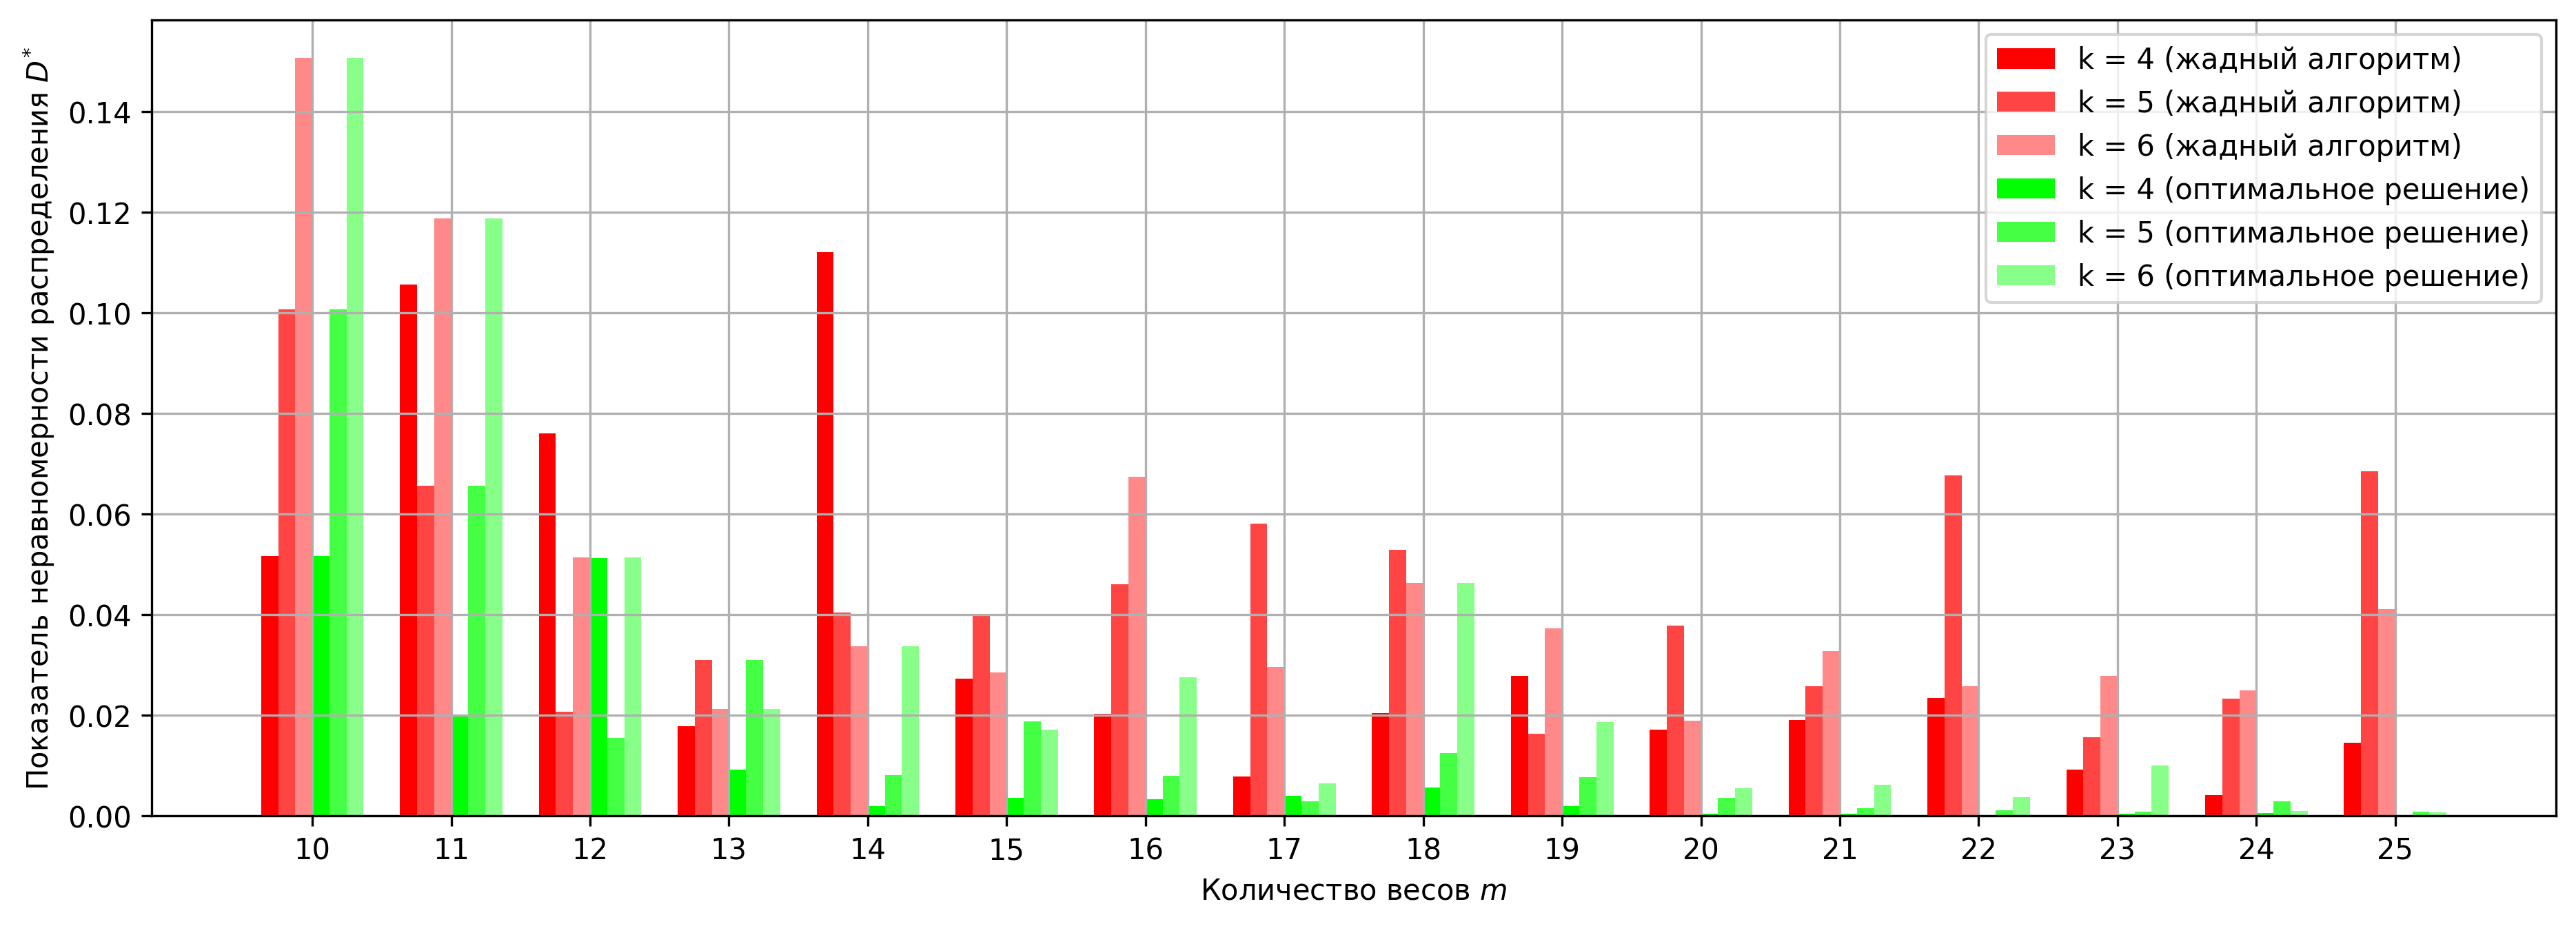
\includegraphics[width=1.0\textwidth]{fig/par_blocks_distr_greedy_opt_cmp_graph.png}
\singlespacing
\captionstyle{center}\caption{Диаграммы сравнения результатов работы жадного алгоритма \\ с оптимальным решением при разбинении множества $m$ весов \\ на $k$ подмножеств.}
\label{fig:par_blocks_distr_greedy_opt_cmp_graph}
\end{figure}

На рис.~\ref{fig:par_blocks_distr_greedy_opt_cmp_graph} представлены диаграммы сравнения результатов работы жадного алгоритма с оптимальным решением, полученные при разбиении $m$ размеров блоков блочно-структурированной расчетной сетки между $k$ процессами при значениях $10 \le m \le 25$, $4 \le k \le 6$.
Из представленных диаграмм можно отметить, что при увеличении количества весов $m$ неравномерность распределения $D^{*}$ снижается, однако результаты работы жадного алгоритма сильно проигрывают оптимальному решению.

Также можно отметить, что высокие значения остаточных членов $r_i$, которые используются при оценке качества разбиения множества $m$ весов на $k$ подмножеств в лемме~\ref{lem:text_2_withcut_lem}, являются индикаторами наличия крупных блоков в расчетной сетке.
При наличии крупных блоков в сетке показатель качества распределения $D$ снижается.
Краевой случай можно наблюдать на расчетной сетке с одним расчетным блоком размера $n$, для такой сетки $D = r_0 = n (1 - \frac{1}{k})$.
Исходя из этого можно заключить, что для повышения эффективности распределения вычислительной нагрузки для блочно-структурированной расчетной сетки необходимо использовать дробление крупных блоков.

\subsubsection{Механизм дробления блоков}

Одним из важнейших для распределения вычислительной нагрузки действий по управлению блочно-структурированной расчетной сеткой при выполнении вычислений на суперкомпьютере является дробление ее блоков \cite{Rybakov2016WithCut}.
Так как при запуске задач на суперкомпьютере постоянно возрастает степень параллельности (используется все больше параллельных процессов обработки блоков сетки), то для сохранения равномерности распределения блоков по вычислительным процессам требуется уметь измельчать блоки.
Блок сетки может быть разделен на два блока по любому из трех измерений: $I$, $J$, $K$.

Кроме блоков сетка содержит другие объекты, которые требуют корректировки после разделения блока.
Сюда относятся интерфейсы, описывающие касание блоков друг друга.
На границе расчетной области граничные условия задаются с помощью специальных объектов, которые также должны быть разделены в случае пересечения их линией разреза блока.
Также должны быть по необходимости разделены области, описывающие начальные условия.
Каждый из этих объектов имеет жесткую привязку к блоку, а значит после дробления может возникнуть
необходимость разделения этого объекта.

Граничные условия и области начальных условий обрабатываются наиболее просто и похожим образом.
Рассмотрим, например, граничные условия в двумерном случае (в координатах $IJ$).

\begin{figure}[ht]
\centering
\begin{tabular}{ll}
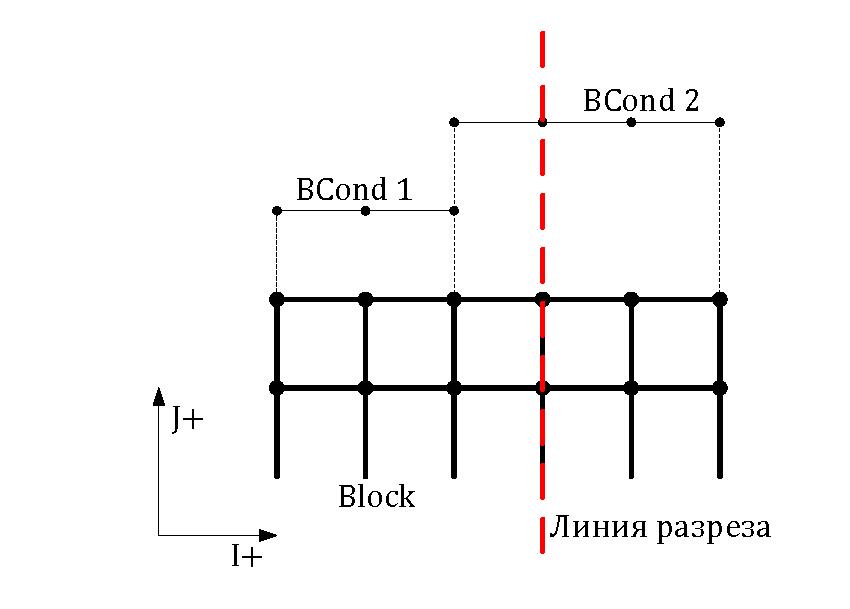
\includegraphics[width=0.48\textwidth]{fig/par_cut-bcond.pdf}
&
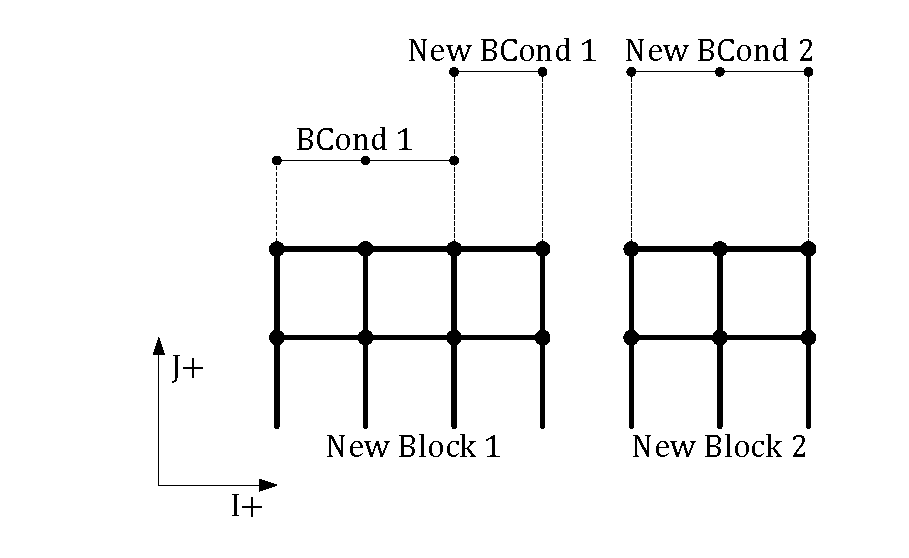
\includegraphics[width=0.48\textwidth]{fig/par_cut-bcond2.pdf}
\end{tabular}
\singlespacing
\captionstyle{center}\caption{Дробление блока может спровоцировать дробление других объектов сетки.}
\label{fig:text_2_withcut_cut_bcond}
\end{figure}

Пусть блок Block должен быть разрезан по направлению $I^{+}$ как показано на рис.~\ref{fig:text_2_withcut_cut_bcond} слева.
Пусть этот блок имеет граничные условия по направлению $J^{+}$.
Тогда возможны два варианта.
Либо линия разреза не пересекает граничное условие, и тогда граничное условие целиком отходит одному из результирующих блоков (BCond 1).
Если же линия разреза проходит через граничное условие, то это граничное условие также должно быть разделено, и его части отойдут двум результирующим блокам (рис.~\ref{fig:text_2_withcut_cut_bcond}, справа).
Такая же ситуация может сложиться в отношении областей начальных условий.
В случае дробления интерфейсов может возникнуть необходимость дробления соседних блоков или повторного деления того же блока (если имеет место самокасание блока).

\subsubsection{Построение равномерного распределения блоков по \mbox{процессам} с дроблением блоков}

Сначала рассмотрим следующую задачу по выделению из блока расчетной сетки части заданного размера при условии минимизации количества дроблений блока.
Пусть есть трехмерный блок размера $a \times b \times c$ ($a > 0$, $b > 0$, $c > 0$).
Требуется определить минимальное количество дроблений, которые необходимо выполнить для того, чтобы выделить из этого блока часть, размера $t \ge 0$ (возможно эта часть будет состоять из нескольких блоков).
Обозначим это минимальное количество дроблений через $P_{a \times b \times c}^t$.

Сначала рассмотрим задачу для одномерного блока размера $a$.
Минимальное количество дроблений для выделения из него части размера $t$ обозначим $P_a^t$.
Для одномерного случая, очевидно, что при $t > a$ решение отсутствует, для $t = 0$ и $t = a$ дробления выполнять не нужно, а для остальных значений $t$ достаточно одного разреза блока.

\begin{equation}\label{eqn:par_pnt_1d}
P_a^t =
	\begin{cases}
		+\infty, & \text{если } t > a \\[-8pt]
		0, & \text{если } (t = 0) \vee (t = a) \\[-8pt]
		1, & \text{если } 0 < t < a
	\end{cases}
\end{equation}

Далее рассмотрим задачу для двумерного случая.
В этом случае рассматривается двумерный блок размера $a \times b$, а минимальное количество дроблений для выделения из него части размера $t$ обозначим через $P_{a \times b}^t$.
Основная идея выделения из блока части размера $t$ заключается в дроблении блока на два новых блока по одному из измерений и выделения из них частей размера $t_1$ и $t - t_1$ соответственно (см. рис.~\ref{fig:par_pnmt_2d}).
Для получения ответа необходимо рассмотреть все возможные варианты первоначального разделения блока на два новых и выбрать тот вариант, который приводит к наименьшему количеству дроблений.
При этом отдельно следует рассмотреть краевые случаи: при $t > ab$ решение отсутствует, при $t = 0$ или $t = ab$ никаких дроблений выполнять не нужно, а для случаев $a = 1$ или $b = 1$ задача сводится к одномерному случаю и вычисление выполняется по формуле \eqref{eqn:par_pnt_1d}.

Исходя из этого, значение $P_{a \times b}^t$ определяется следующим образом:

\begin{equation}\label{eqn:par_pnmt_2d}
P_{a \times b}^t =
	\begin{cases}
		+\infty, & \text{если } t > ab \\
		0, & \text{если } (t = 0) \vee (t = ab) \\
		P_b^t, & \text{если } a = 1 \\
		P_a^t, & \text{если } b = 1 \\
		\begin{aligned}
			\min\big[
				& \min_{\substack{1 \le a_1 < a \\ 0 \le t_1 < t}}{\{P_{a_1 \times b}^{t_1} + P_{(a - a_1) \times b}^{t - t_1}\}}, \\[-8pt]
				& \min_{\substack{1 \le b_1 < b \\ 0 \le t_1 < t}}{\{P_{a \times b_1}^{t_1} + P_{a \times (b - b_1)}^{t - t_1}\}}
			\big] + 1
		\end{aligned}, &
			\begin{aligned}
				\text{если } & (\min(a, b) > 1) \\[-10pt]
				& \wedge (0 < t < ab)
			\end{aligned}
	\end{cases}
\end{equation}

Для трехмерного случая значение $P_{a \times b \times c}^t$ вычисляется аналогично с помощью дробления блока по одному из трех измерений и с использованием значений для двумерного случая:

\begin{equation}\label{eqn:par_pnmkt_3d}
P_{a \times b \times c}^t =
	\begin{cases}
		+\infty, & \text{если } t > abc \\
		0, & 
			\begin{aligned}
				\text{если } & (t = 0) \\[-10pt]
				& \vee (t = abc)
			\end{aligned} \\
		P_{b \times c}^t, & \text{если } a = 1 \\
		P_{a \times c}^t, & \text{если } b = 1 \\
		P_{a \times b}^t, & \text{если } c = 1 \\
		\begin{aligned}
			\min\big[
				& \min_{\substack{1 \le a_1 < a \\ 0 \le t_1 < t}}{\{P_{a_1 \times b \times c}^{t_1} + P_{(a - a_1) \times b \times c}^{t - t_1}\}}, \\[-8pt]
				& \min_{\substack{1 \le b_1 < b \\ 0 \le t_1 < t}}{\{P_{a \times b_1 \times c}^{t_1} + P_{a \times (b - b_1) \times c}^{t - t_1}\}}, \\[-8pt]
				& \min_{\substack{1 \le c_1 < c \\ 0 \le t_1 < t}}{\{P_{a \times b \times c_1}^{t_1} + P_{a \times b \times (c - c_1)}^{t - t_1}\}}
			\big] + 1
		\end{aligned}, & 
			\begin{aligned}
				\text{если } & (\min(a, b, c) > 1) \\[-10pt]
				& \wedge (0 < t < abc)
			\end{aligned}
	\end{cases}
\end{equation}

\begin{figure}[ht]
\centering
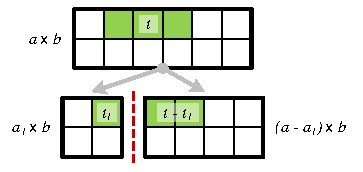
\includegraphics[width=0.6\textwidth]{fig/par_pnmt_2d.pdf}
\singlespacing
\captionstyle{center}\caption{Рекурсивное выделение из блока $a \times b$ части размера $t$.}
\label{fig:par_pnmt_2d}
\end{figure}

Используя формулы \eqref{eqn:par_pnt_1d} -- \eqref{eqn:par_pnmkt_3d}, можно вычислить значения $P_{a \times b \times c}^t$.
Прямое вычисление этих значений сопряжено с высокими вычислительными затратами, экспоненциально возрастающими с ростом $a$, $b$, $c$ и $t$.
Для ускорения вычислений можно использовать некоторые простые свойства $P_{a \times b \times c}^t$, сформулированные в следующей лемме для трехмерного случая:

\begin{lemma}\label{lem:par_pnmkt_properties}
Значения $P_{a \times b \times c}^t$ минимального количества разбиений блока расчетной сетки $a \times b \times c$ для выделения части размера $t$ обладают следующими свойствами:
\begin{enumerate}[noitemsep,topsep=0pt,parsep=0pt,partopsep=0pt]
\item Симметричность относительно аргументов $a$, $b$, $c$. Верны соотношения $P_{a \times b \times c}^t = P_{a \times c \times b}^t = P_{b \times a \times c}^t = P_{b \times c \times a}^t = P_{c \times a \times b}^t = P_{c \times b \times a}^t$. 
\item Симметричность относительно аргумента $t$. Для всех допустимых значений параметров и при условии $0 \le t \le abc$ имеет место соотношение $P_{a \times b \times c}^t = P_{a \times b \times c}^{abc - t}$.
\item Ограниченность. Для всех допустимых значениях параметров и при условии $0 \le t \le abc$ верно ограничение $P_{a \times b \times c}^t \le 5$.
\end{enumerate}
\end{lemma}

Первое свойство следует непосредственно из того, что все блоки $a \times b \times c$, $a \times c \times b$, $b \times a \times c$, $b \times c \times a$, $c \times a \times b$, $c \times b \times a$ являются одним и тем же блоком с точностью до порядка перечисления размеров сторон.

Второе свойство следует из того, что отделение от блока $a \times b \times c$ (имеющего размер $abc$) части размера $t$, означает разделение его на две части -- размерами $t$ и $abc - t$.

Ограниченность $P_a^t$ и $P_{a \times b}^t$ следует непосредственно из формул \eqref{eqn:par_pnt_1d} -- \eqref{eqn:par_pnmt_2d}, из которых нетрудно видеть, что $P_a^t \le 1$ при $t \le a$, $P_{a \times b}^t \le 3$ при $t \le ab$.
Из формулы \eqref{eqn:par_pnmkt_3d} можно получить оценку $P_{a \times b \times c}^t \le 7$.
Для доказательства более строгой оценки $P_{a \times b \times c}^t \le 5$ построим разбиение, на которое гарантированно не потребуется более пяти разрезов.
Если $t = 0$ или $t = abc$, то ничего не делаем, иначе продолжаем.
Первым разрезом отрежем от блока $a \times b \times c$ часть $\lfloor \frac{t}{bc} \rfloor \times b \times c$.
Нам осталось выделить из блока $\left(a - \lfloor \frac{t}{bc} \rfloor\right) \times b \times c$ часть размера $t_1 = t \bmod bc$.
Если $t_1 = 0$, то останавливаемся, иначе продолжаем.
Вторым разрезом от блока $\left(a - \lfloor \frac{t}{bc} \rfloor\right) \times b \times c$ отрезаем $1 \times b \times c$ и далее работаем с ним.
Третьим разрезом от блока $1 \times b \times c$ отрезаем часть $1 \times \lfloor \frac{t_1}{c} \rfloor \times c$.
Теперь осталось от блока $1 \times \left( b - \lfloor \frac{t_1}{c} \rfloor \right) \times c$ отрезать часть размера $t_2 = t_1 \bmod c$.
Если $t_2 = 0$, то останавливаемся, иначе продолжаем.
Четвертым разрезом от блока $1 \times \left( b - \lfloor \frac{t_1}{c} \rfloor \right) \times c$ отрезаем $1 \times 1 \times c$ и уже от него пятым разрезом отрезаем недостающую часть $t_2$.
В результате выполненных дроблений выделена часть
\begin{multline}
	\Bigl \lfloor \frac{t}{bc} \Bigr \rfloor bc + \Bigl \lfloor \frac{t_1}{c} \Bigr \rfloor c + t_2 =
	\left(t - (t \bmod bc)\right) \\ + \left((t \bmod bc) - ((t \bmod bc) \bmod c)\right) + ((t \bmod bc) \bmod c) = t,
\end{multline}
откуда следует требуемое утверждение.
$\blacksquare$\\

\begin{figure}[ht]
\centering
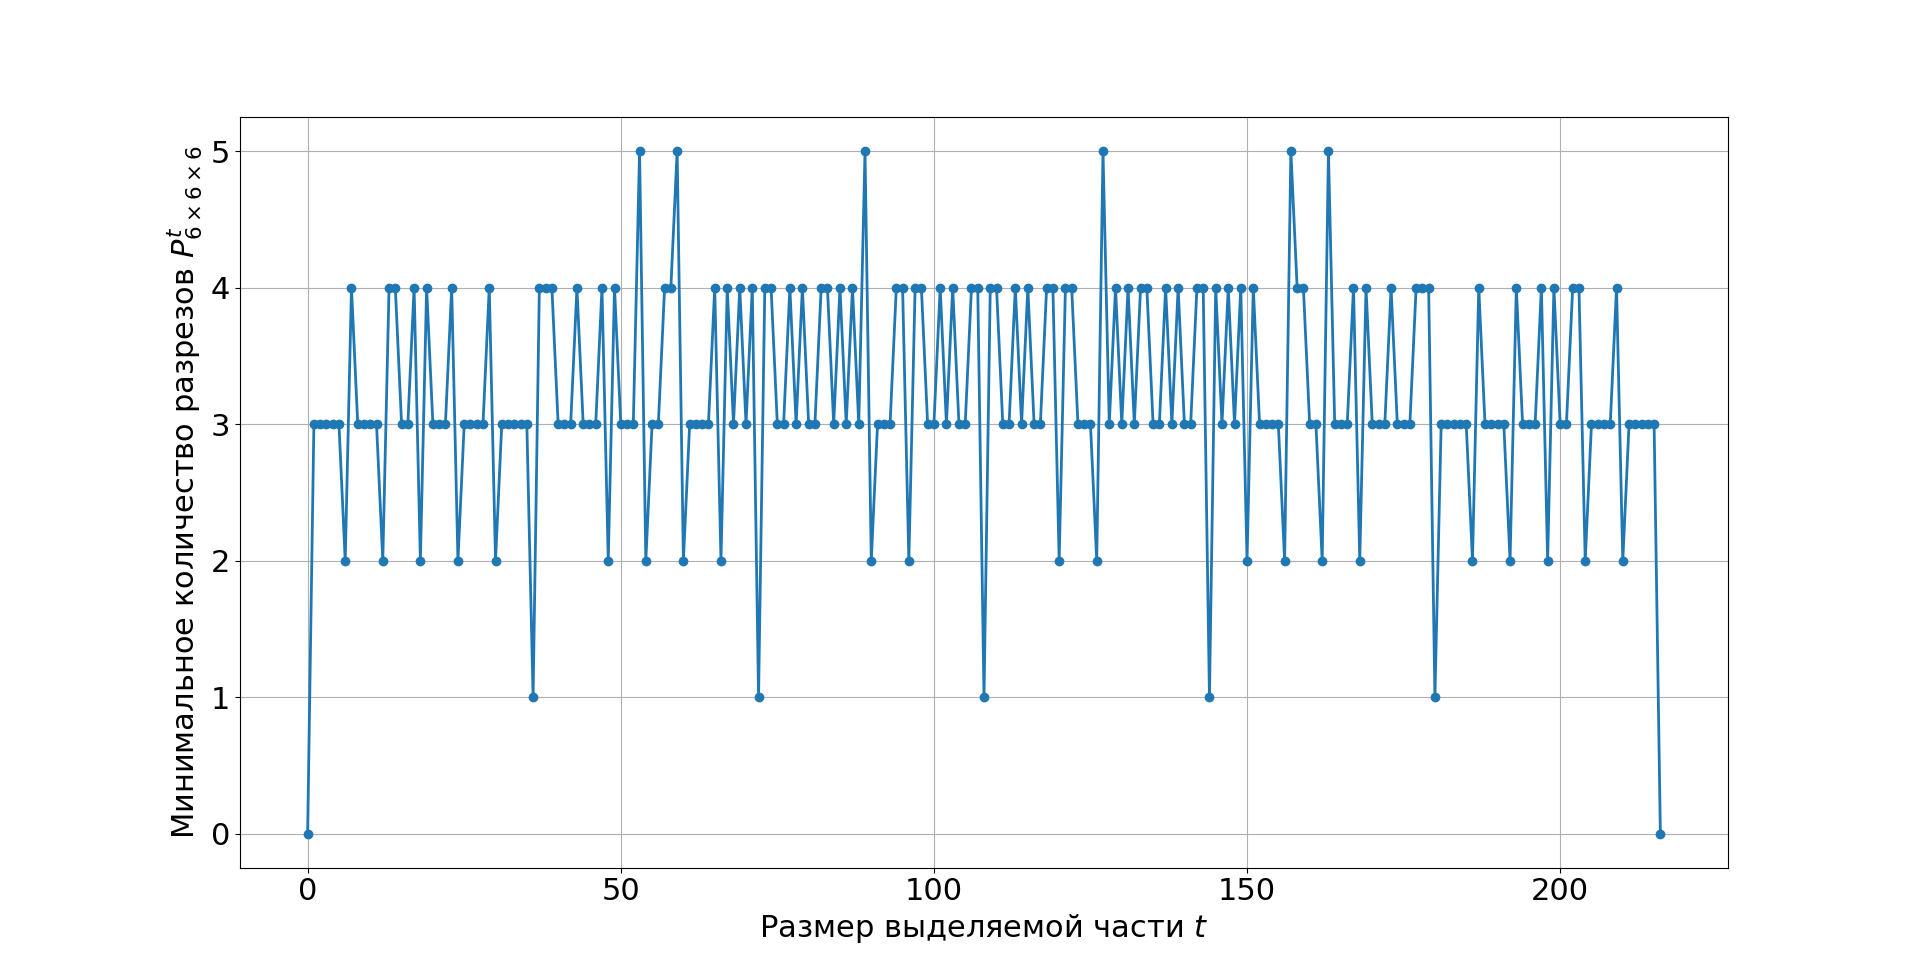
\includegraphics[width=1.0\textwidth]{fig/par_min_cuts_for_extract_part_chart.png}
\singlespacing
\captionstyle{center}\caption{График зависимости $P_{6 \times 6 \times 6}^t$ от $0 \le t \le 6^3$.}
\label{fig:par_pnmkt_chart}
\end{figure}

На рис.~\ref{fig:par_pnmkt_chart} приведен характерный вид графика функции $f(t) = P_{n \times n \times n}^t$ на примере $n = 6$.
На приведенном рисунке наиболее распространенными значениями $P_{6 \times 6 \times 6}^t$ являются значения 3 и 4.

Из свойств 1 и 2 леммы~\ref{lem:par_pnmkt_properties} следует, что достаточно вычислить значения $P_{a \times b \times c}^t$ при ограничениях $a \ge b \ge c$, $t \le abc$.
Для возможности эффективного вычисления $P_{a \times b \times c}^t$ необходимо использовать принцип динамического программирования, то есть сохранение ранее вычисленных значений для последующего повторного использования в рекурсивных вызовах.
Размер памяти, требуемой для сохранения результатов при ограничениях $a \ge b \ge c$, $t \le abc$ может быть вычислен как
\begin{equation}
	\sum_{a_i = 1}^{a}{ \sum_{b_i = 1}^{a_i}{ \sum_{c_i = 1}^{b_i}{ \frac{a_i b_i c_i}{2} } } } = \frac{1}{96} a^6 + o(a^6),
\end{equation}
что говорит о слишком больших накладных расходах по памяти.

Если предположить, что мы можем вычислить все требуемые значения $P_{a \times b \times c}^t$, а также все координаты требуемых разрезов блоков для выделения из блока $a \times b \times c$ части размера $t$, то равномерное распределение блоков расчетной сетки между произвольным количестом вычислительных процессов, очевидно, может быть получено с показателем $D = 0$ (если $k \mid n$).
При этом, в общем случае, для каждого процесса кроме последнего необходимо будет выполнять дробление блока для выделения из него части требуемого размера.
Общее количество разрезов, необходимое для достижения равномерного распределения можно оценить, что сформулировано в следующей лемме:

\begin{lemma}
При распределении произвольного количества блоков расчетной сетки с суммарным количеством ячеек $n$ по $k$ партициям и выполнении условия $k \mid n$ равномерное распределение с показателем $D = 0$ может быть достигнуто с использовнием не более $5(k - 1)$ разрезов блоков.
\end{lemma}

Справедливость утверждения следует непосредственно из того, что в худшем случае для каждой партиции кроме последней потребуется выделение из некоторого блока части требуемого размера (для достижения наполнения этой партиции ровно $\frac{n}{k}$ ячейками) и на каждый такой блок потребуется не более 5 разрезов, согласно лемме~\ref{lem:par_pnmkt_properties}.
$\blacksquare$\\

Рассмотренный вариант построения распределения блоков расчетной сетки по партициям с использованием дробления блоков хоть и приводит к равномерному распределению с показателем $D = 0$, однако обладает рядом недостатков, что делает его непригодным при использовании в практических приложениях.
Поиск значений $P_{a \times b \times c}^t$ требует слишком высоких затрат по времени вычисления и по памяти для хранения уже вычисленных значений.
С учетом выполненных оценок и предположений количество разрезов блоков, требуемых для построения распределения блоков по партициям, кратно превосходит количество партиций.
В процессе дробления блоков могут появляться блоки со слишком маленькими размерами по одному или нескольким измерениям, что приводит к возрастанию теневых зон и увеличению объема межпроцессных обменов.

Ввиду сделанных выводов требуется рассмотрение приближенных методов распределения блоков между партициями, которые могут быть использованы на практике.
Будем вести поиск таких методов распределения, при которых показатель $D$ остается на достаточно низком уровне при существенном сокращении количества дроблений блоков.

\subsubsection{Дробление наиболее крупных блоков пополам}

Рассмотрим наиболее простую стратегию распределения блоков по партициям с использованием дробления блоков.
Для распределения блоков будем использовать жадный алгоритм.
Если после распределения блоков с использованием жадного алгоритма показатель $D^{*}$ окажется выше требуемого значения, то выполним разрез наиболее крупного блока пополам по наиболее протяженному направлению и повторим распределение с помощью жадного алгоритма.
Без ограничения общности будет считать, что размеры блока отсортированы по убыванию (то есть наибольшим размером блока является размер $a$).
Для дробления блока будем использовать следующее обозначение $\{b_1, b_2\} = b.cut(i)$, означающее дробление блока $b$ на два блока путем разреза по наиболее протяженному измерению в позиции $i$ (при котором сторона длины $a$ делится на две части размерами $i$ и $a - i$).

\begin{algo}\label{alg:par_distr_halfmaxblock}
Алгоритм распределения множества блоков по партициям с помощью дробления наибольших блоков (\texttt{DistributeHalfMaxBlock}).
\begin{algorithm}
\DontPrintSemicolon
\KwInput{$B$ -- множество блоков ($|B| = m$), $k$ -- количество результирующих партиций, $\epsilon$ -- допустимое значение показателя $D^{*}$.}
\KwOutput{$P$ -- множество результирующих партиций.}
\Fn{\texttt{DistributeHalfMaxBlock}($B$, $k$, $\epsilon$)}
{
	\While{$true$}
	{
		$P \leftarrow \texttt{DistributeGreedy}(B, k)$\;
		\If{$P.D^{*} \le \epsilon$}
		{
			\KwRet $P$\;
		}
		\Else
		{
			$b \leftarrow B.max$\;
			$B \leftarrow (B \setminus \{b\}) \cup b.cut(\lfloor \frac{b.a}{2} \rfloor)$\;
		}
	}
}
\end{algorithm}
\end{algo}

Приведенный алгоритм гарантированно завершает работу при $\epsilon \ge \frac{\lceil \mu \rceil - \mu}{\mu}$, где $\mu = \frac{B.w}{k}$, так как значение $P.D^{*} = \frac{\lceil \mu \rceil - \mu}{\mu}$ может быть достигнуто при дроблении всех блоков до единичного размера.
Количество требуемых дроблений сильно зависит от конкретных размеров блоков и возрастает при уменьшении параметра $\epsilon$.
Если количество разрезов блоков принять за $\sigma \ge 1$, то сложность алгоритма можно оценить как $O(m \log m + \sigma(m \log k + k + \sigma))$.
$\blacksquare$\\

Этот алгоритм распределения блоков сетки между вычислительными процессами с использованием дробления был протестирован на различных расчетных сетках.
Ниже представлен результат тестирования на двух расчетных сетках.

Первая рассматриваемая сетка содержит 13 блоков, 80 интерфейсов, 148 граничных условий, 13 областей начальных условий и 5,75 млн ячеек, размер вычислительной окрестности равен 3.
Вторая рассматриваемая сетка содержит 300 блоков, 1796 интерфейсов, 1643 граничных условия, 300 областей начальных данных и 94,34 млн ячеек.
Размер вычислительной окрестности также равен 3.

Для этих сеток были проведено распределение блоков для 128 вычислительных процессов.
Статистика распределения блоков по вычислительным процессам для двух различных вариантов: без использования дробления блоков и с использованием дроблений для достижения показателя неравномерности распределения распределения не более $D^{\%} = 10\%$ (см. рис.~\ref{fig:text_2_withcut_charts}).

\begin{figure}[ht]
\centering
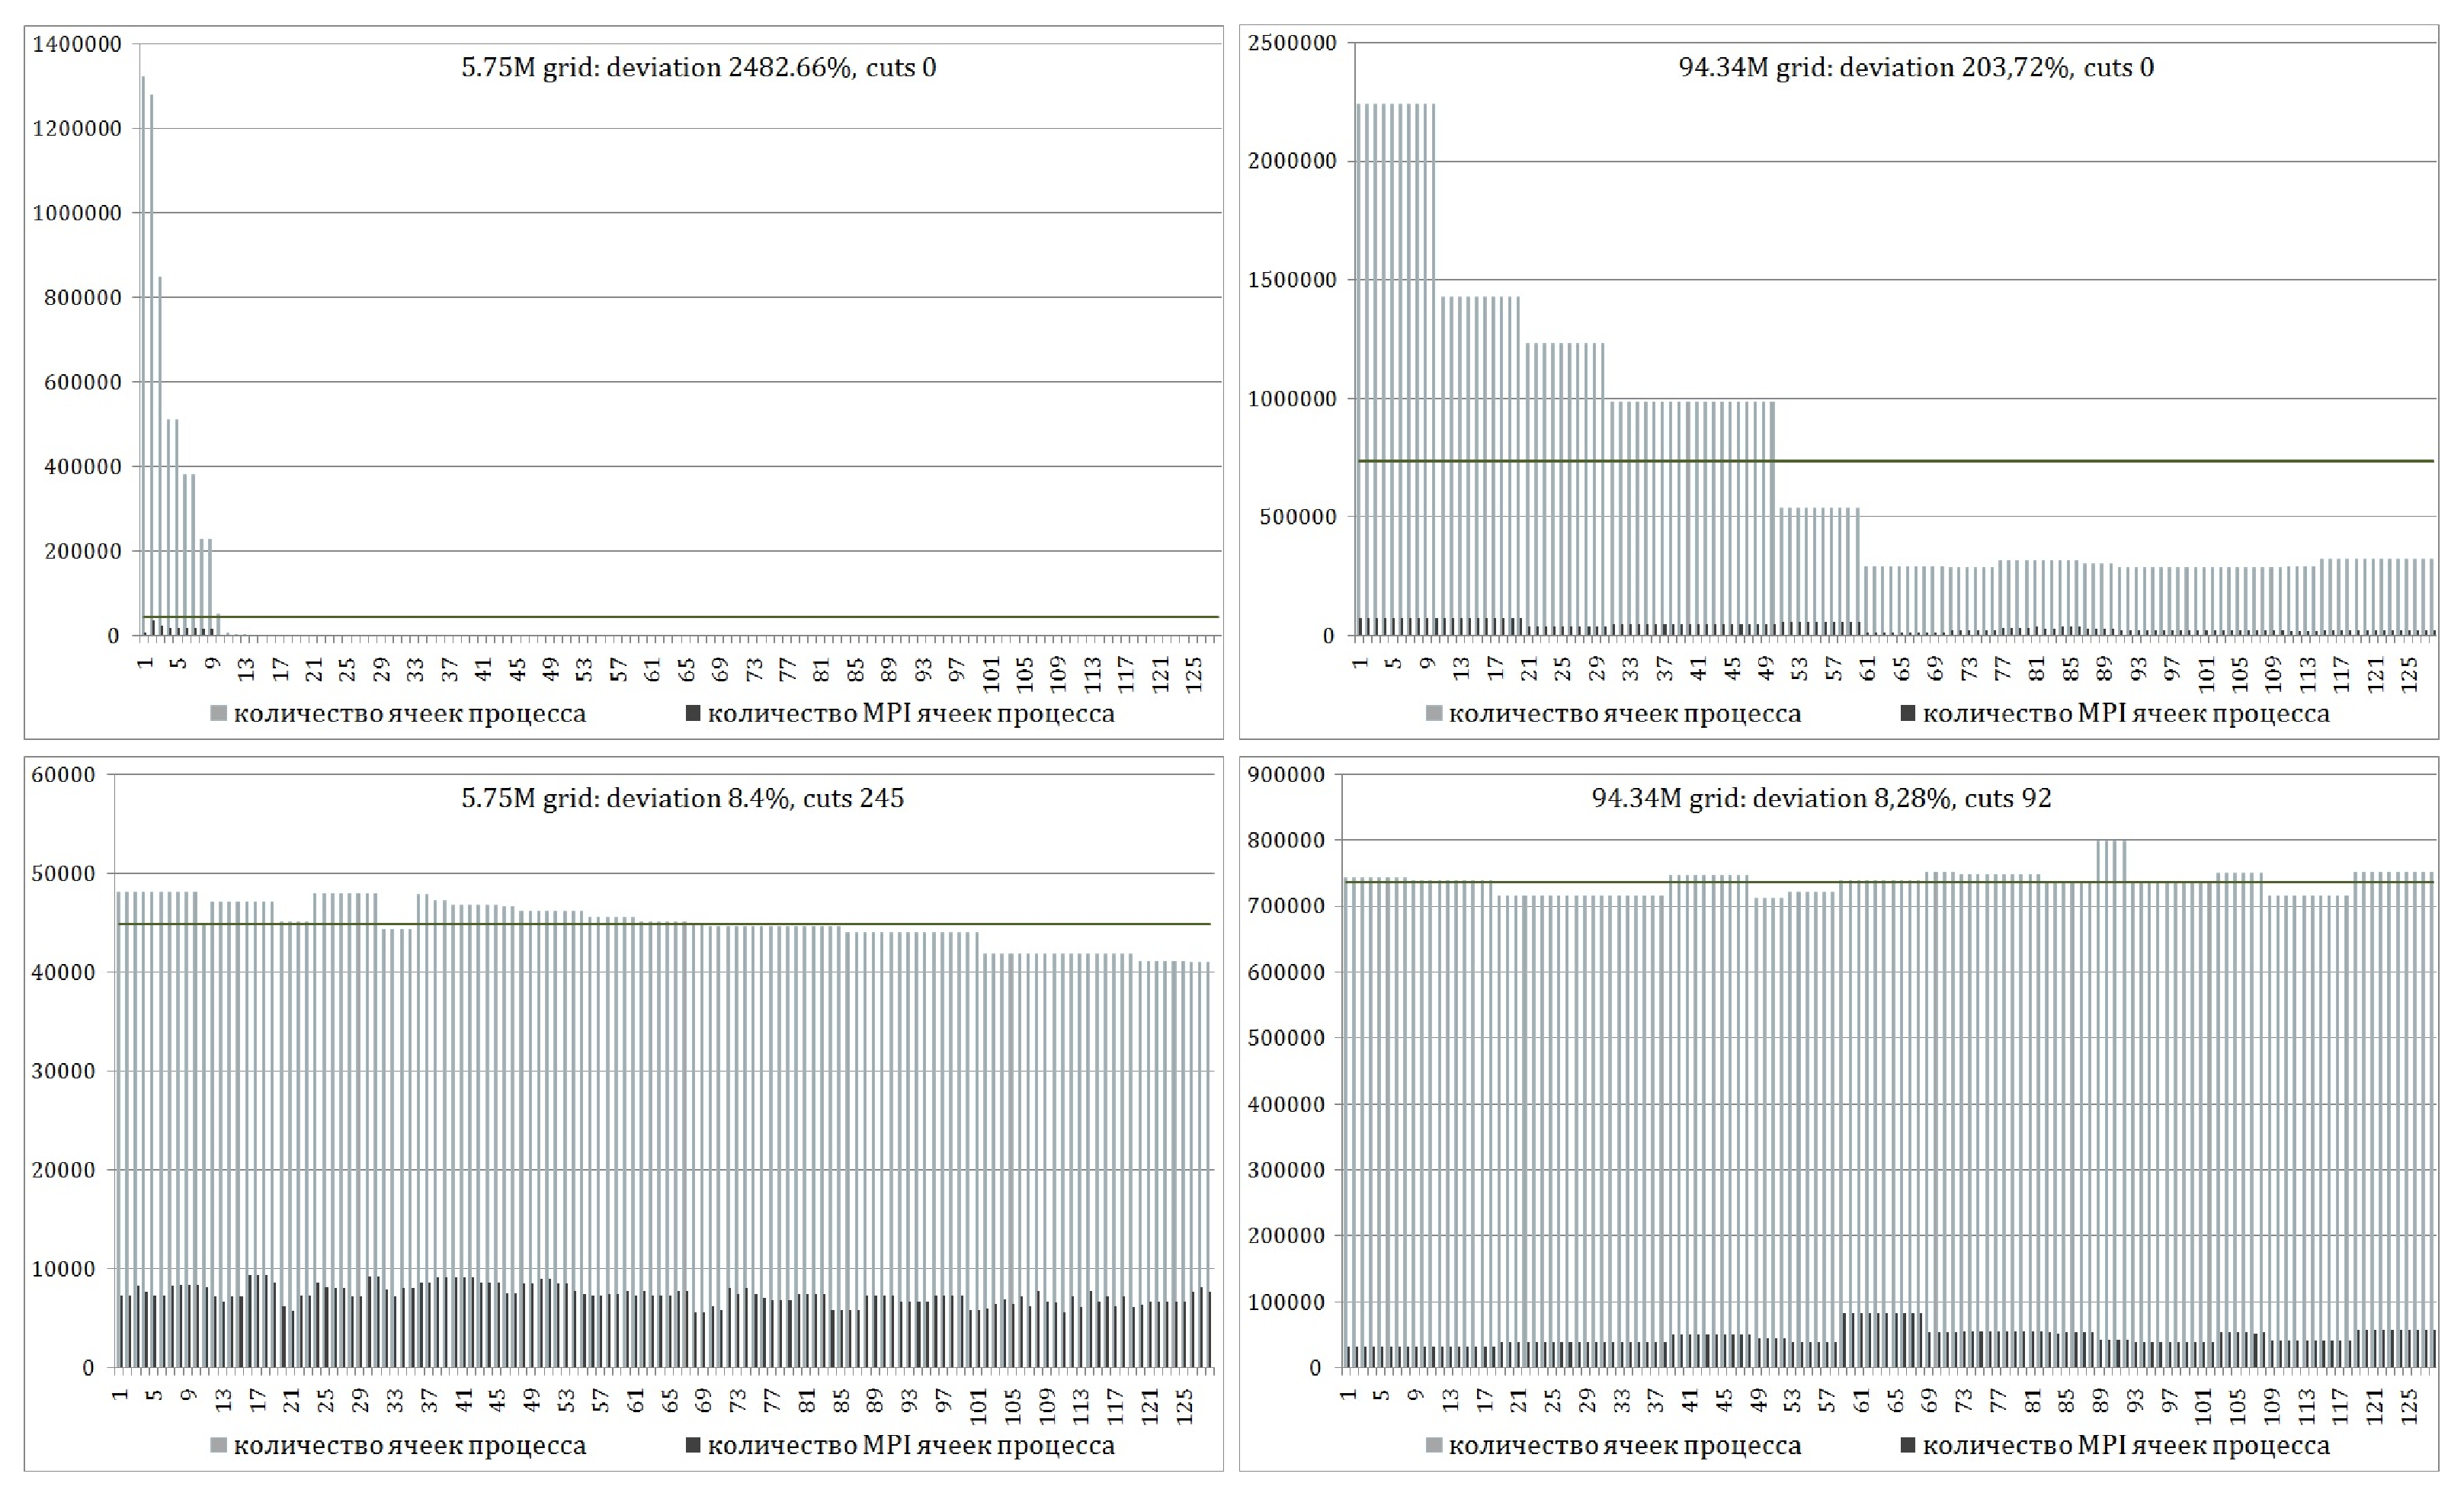
\includegraphics[width=1.0\textwidth]{fig/par_withcut-charts.pdf}
\singlespacing
\captionstyle{center}\caption{Распределение блоков тестовых сеток (5,75 млн ячеек -- слева, 94,34 млн ячеек -- справа) без дробления (наверху) и с дроблением с допустимым отклонением $D^{\%} = 10\%$ (снизу).}
\label{fig:text_2_withcut_charts}
\end{figure}

Предложенный алгоритм распределения блоков расчетной сетки между вычислительными процессами приводит к более равномерной загрузке вычислительных ресурсов суперкомпьютерного кластера, что повышает эффективность его использования в расчетных задачах.
Часто применение такого подхода на большом количестве процессов приводит к кратному ускорению вычислений.
Особенно это актуально для сеток содержащих небольшое количество блоков или для сеток, имеющих ярко выраженные крупные блоки.

Негативным фактором применения дробления блоков является увеличение количества блоков и количества граничных ячеек, что приводит к увеличению объема данных межпроцессных обменов.
Проанализируем, как увеличение количества блоков и граничных ячеек влияет на производительность вычислений.
При этом последовательность дробления блоков сетки для достижения требуемого целевого значения показателя $D^{\%}$ при распределении блоков между $k$ процессами будем называть подготовкой сетки.

Для анализа эффективности распределения блоков по вычислительным процессам с использованием дробления блоков был поставлен эксперимент по выполнению газодинамических расчетов методом RANS/ILES\label{abbr:rans-2}\label{abbr:iles-2} на блочно-структурированной расчетной сетке, содержащей 10,7 млн ячеек \cite{Savin2019RANS}.
Эксперимент проводился сегменте суперкомпьютера, состоящем из узлов, каждый из которых содержит по одному микропроцессору Intel Xeon Phi KNL\label{abbr:knl-1}.
Перед вычислениями выполнялась подготовка расчетной сетки для $k = 16$, $k = 32$ и $k = 64$ путем распределения вычислительной нагрузки с дроблением наиболее крупных блоков сетки.
При подготовке расчетной сетки использовалось допустимое отклонение $D^{\%} = 10\%$, для подготовки вычислений для $k = 64$ дополнительно использовалось допустимое отклонение $D^{\%} = 1\%$ (характеристики расчетных сеток приведены в таблице~\ref{tbl:text_2_withcut}).

\begin{table}[!ht]
\centering
\singlespacing
\captionstyle{center}\caption{Характеристики используемых расчетных сеток, после подготовки для разных значений $k$ и $D^{\%}$.}
\bigskip
\label{tbl:text_2_withcut}
\begin{tabular}{ | c | c | c | c | c | }
  \hline
  Расчетная сетка & Блоки & Интерфейсы & Граничые условия \\ \hline\hline
  исходная сетка & 30 & 152 & 204 \\ \hline\hline
  \makecell{подготовленная сетка \\ $k = 16$, $D^{\%} = 10\%$} & 39 & 224 & 218 \\ \hline
  \makecell{подготовленная сетка \\ $k = 32$, $D^{\%} = 10\%$} & 54 & 340 & 248 \\ \hline
  \makecell{подготовленная сетка \\ $k = 64$, $D^{\%} = 10\%$} & 170 & 982 & 429 \\ \hline\hline
  \makecell{подготовленная сетка \\ $k = 64$, $D^{\%} = 1\%$} & 383 & 2356 & 682 \\ \hline
\end{tabular}
\end{table}

\begin{figure}[ht]
\centering
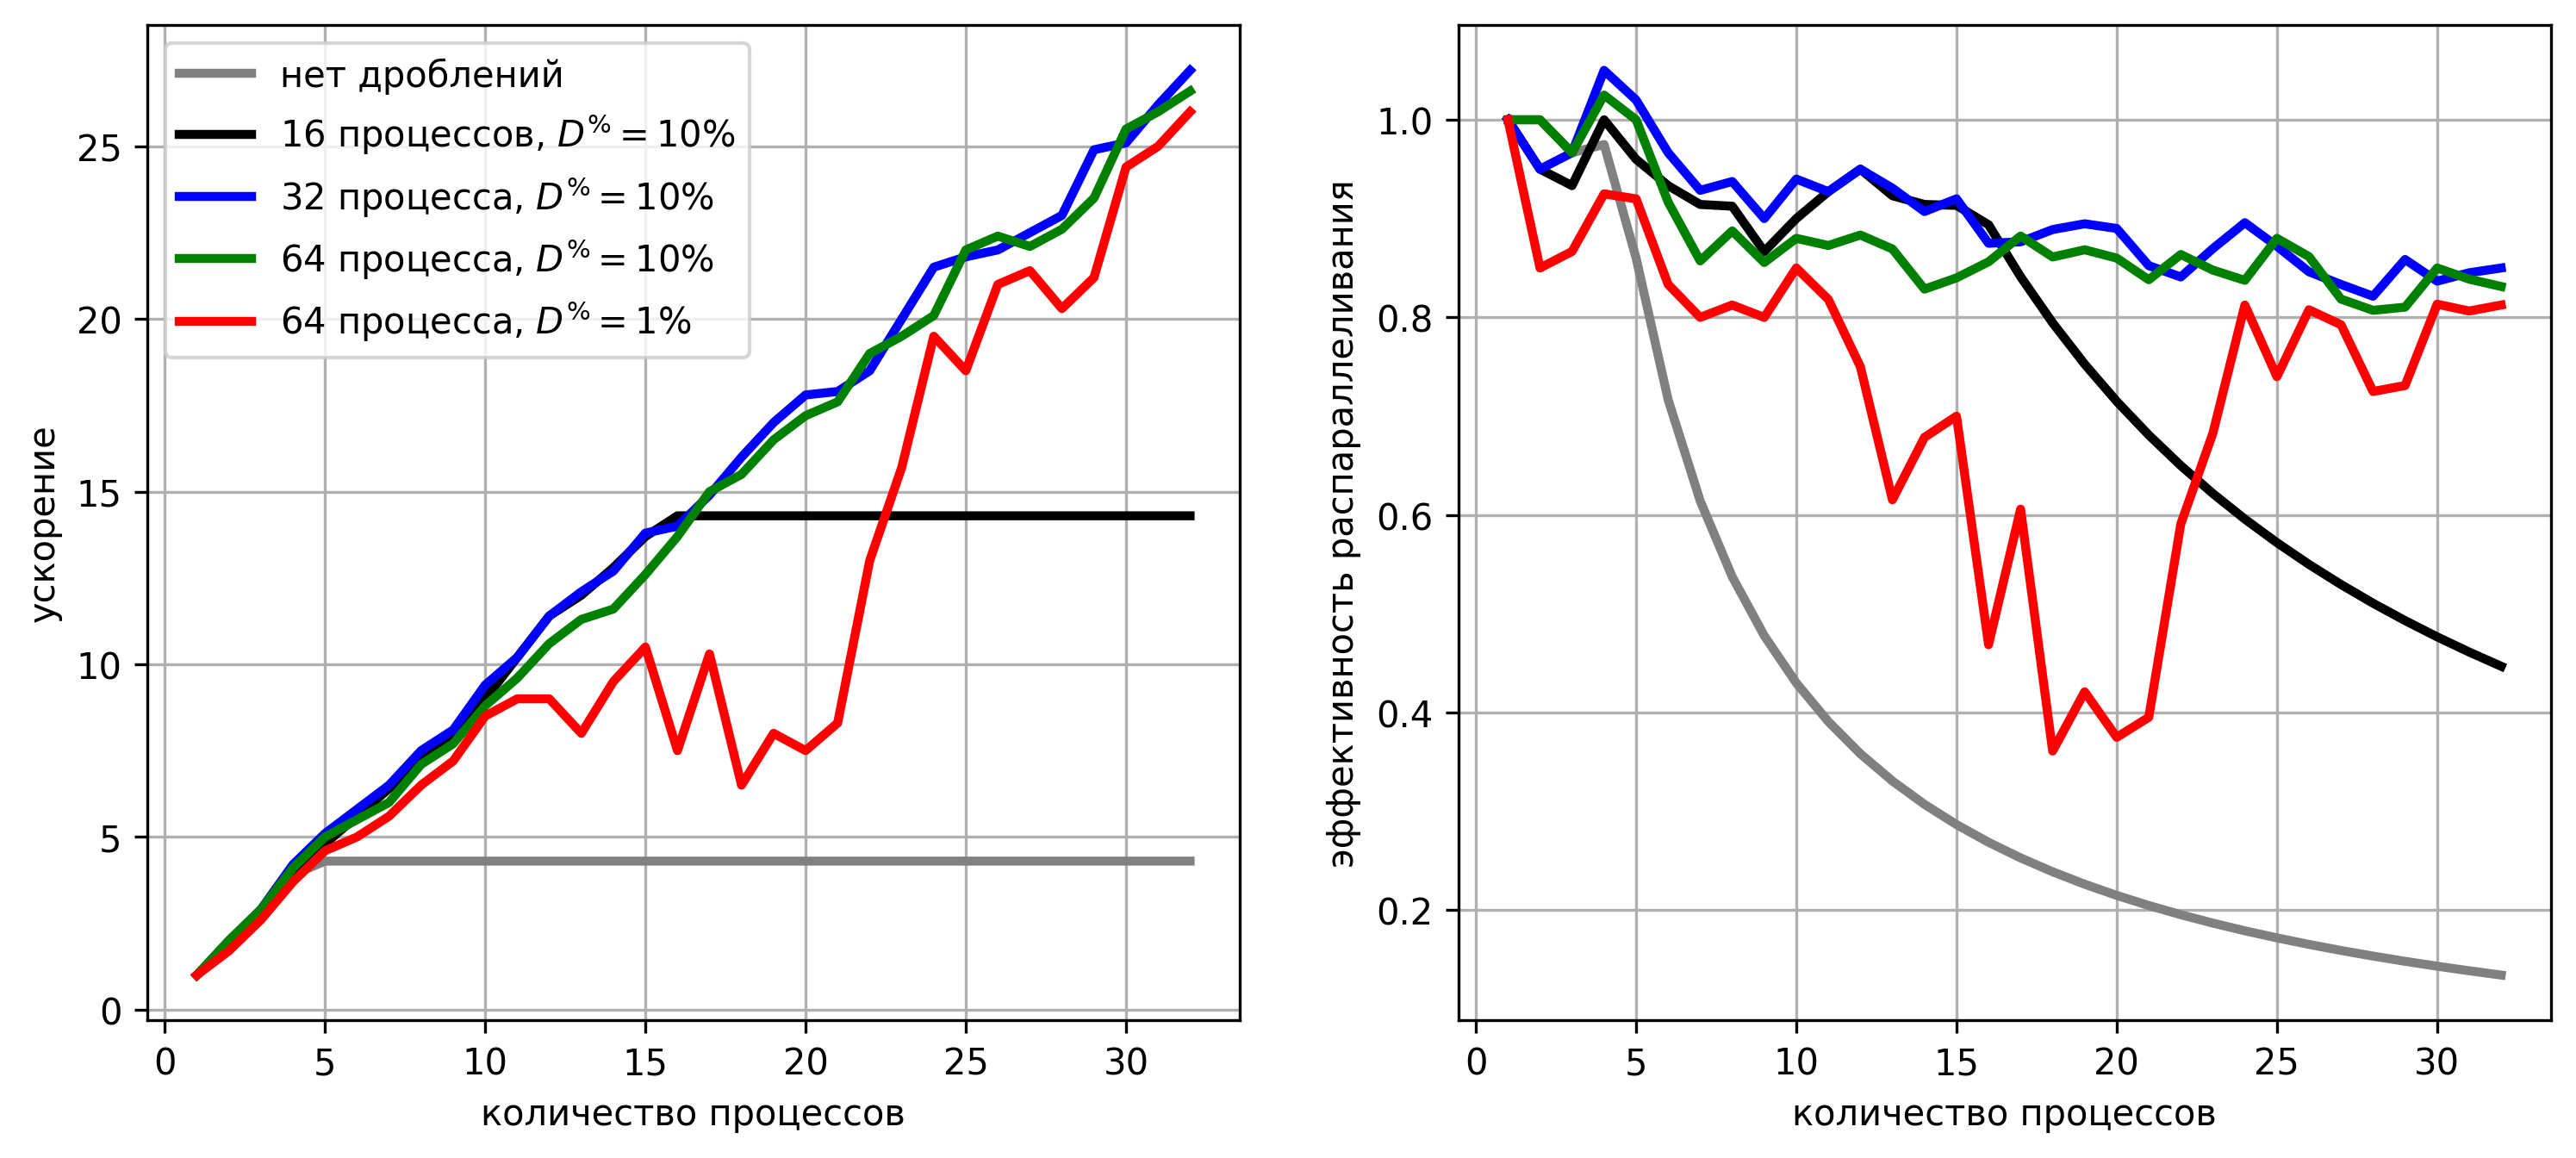
\includegraphics[width=1.0\textwidth]{fig/par_scaling3.png}
\singlespacing
\captionstyle{center}\caption{Масштабирование вычислений при различных параметрах подготовки сетки на 1-32 микропроцессорах Intel Xeon Phi KNL.}
\label{fig:text_2_withcut_scaling3}
\end{figure}

На рис.~\ref{fig:text_2_withcut_scaling3} представлены результаты численных экспериментов на сегменте суперкомпьютера, состоящем из узлов, каждый из которых содержит по одному микропроцессору Intel Xeon Phi KNL.
При проведении расчетов на каждом узле запускался один MPI\label{abbr:mpi-4} процесс.
Количество узлов менялось от 1 до 32.
Проанализируем графики ускорения вычислений, представленные на рис.~\ref{fig:text_2_withcut_scaling3}.

Для вычислений на неподготовленной сетке (соответствует графику "нет дроблений") наблюдается ускорение для количества процессов до 5.
Далее ускорение остается на одной и той же отметке (около 4,3) и не меняется при дальнейшем увеличении количества узлов.
Это связано с наличием крупного блока, который мешает равномерному распределению вычислительной нагрузки.

При подготовке сетки для $k = 16$ (черный график) ускорение также останавливается, но на более высокой отметке (в районе 14,0).
Это также связано с наличием крупного блока, но его размер меньше, чем в случае отказа от дроблений (наиболее крупный блок был раздроблен, что привело к эффективному распределению вычислительной нагрузки для 16 процессов, однако для большего количества процессов размер этого блока препятствует равномерному распределению блоков по процессам).

При подготовке сетки для $k = 32$ и $k = 64$ с допустимым отклонением $D^{\%} = 10\%$ (синий и зеленый графики соответственно) получаем примерно одинаковое возрастание ускорения вычислений с ростом количества узлов.
Это говорит о том, что при подготовка сетки для большего количества процессов, чем реально будет использоваться для запусков, избыточно.

При подготовке сетки для $k = 64$ с допустимым отклонением $D^{\%} = 1\%$ (красный график) наблюдается сильная деградация ускорения и эффективности распараллеливания при использовании количества узлов от 10 до 25.
Это связано с сильным возрастанием количества блоков, граничных ячеек, что привело к увеличению объема данных при межпроцессных обменах.

Из графиков, приведенных на рис.~\ref{fig:text_2_withcut_scaling3}, можно сделать вывод, что при использовании распределения вычислительной нагрузки с дроблением блоков целесообразно предерживаться двух эвристических правил.
Во-первых, подготовку расчетной сетки не следует производить для количества процессов, больше того, которое реально будет использоваться при запусках.
Во-вторых, не стоит выбирать слишком низкий показатель допустимого отклонения $D^{\%}$, так как в случае слишком низкого значения этого показателя равномерность распределения вычислительной нагрузки будет нивелирована возрастанием объема межпроцессных обменов.

Так как подготовка расчетной сетки с помощью дробления наиболее крупных блоков при снижении показателя $D^{\%}$ приводит к сильному увеличению количества блоков и объема данных межпроцессных обменов, то требуется использование других подходов к дроблению блоков сетки с целью уменьшения количества производимых разрезов блоков.

\subsubsection{Стратегия дробления блоков, уменьшающая количество \mbox{разрезов}}

Для устранения крупных блоков без лишних дроблений предлагается алгоритм распределения блоков расчетной сетки по партициям с использованием дробления блоков и уменьшающий количество дроблений \cite{Bendersky2017Eff,Bendersky2018Block}.
Прежде всего определим, на какие части может быть разрезан конкретный блок.
Без ограничения общности будем считать, что размеры блока $b$ отсортированы по убыванию, и сторона по первому измерению $b.a$ является наибольшей.

На возможные разрезы блока будем накладывать следующие ограничения.
Во первых, будем выполнять разрезы только по наиболее протяженному измерению (то есть разбивать наибольшую сторону размера $b.a$ на две части размера $a_1$ и $b.a - a_1$), так как это приводит к уменьшению количества интерфейсных ячеек.
Для запрета появления слишком тонких блоков будем запрещать выполнять разрезы блока слишком близко к границе.
Для этого вводится параметр $\delta$, по которому разрешается деление блока только в сегменте $[\delta, b.a - \delta]$.
Вводится еще одно ограничение, не позволяющее производить слишком мелкие блоки, -- наименьшее допустимое количество ячеек в результирующем блоке, при котором разрешено дробление, это ограничение будем обозначать $\Delta$.

\begin{definition}
Позицию разреза $i$ блока $b$ будем называть допустимой, если $i \in [\delta, b.a - \delta]$ и $\min(i, b.a - i)\frac{b.w}{b.a} \ge \Delta$ (то есть разрез выполнен вдали от границы блока и не порождает блоки маленького размера).
\end{definition}

Для реализации алгоритма с уменьшением количества дроблений блоков рассмотрим четыре основные операции, которые будем в дальнейшем использовать.

Первая операция: для заданного множества блоков $B$ и множества партиций $P$ найти такой блок $b \in B$ и партицию $p \in P$, что величина $p.w + b.w$ является максимально возможной, но не превышающей заданное значение $\tau$.
Эту операцию будем называть заполнением партиции целым блоком снизу (\texttt{FillFullUnder}).

Вторая операция: для заданного множества блоков $B$ и множества партиций $P$ найти такой блок $b \in B$ и партицию $p \in P$, а также допустимую позицию разреза $i$, что величина $p.w + b.w \frac{i}{b.a}$ является максимально возможной, но не превышающей заданное значение $\tau$.
Эту операцию будем называть заполнением партиции частью блока снизу (\texttt{FillPartUnder}).

Третья операция: для заданного множества блоков $B$ и множества партиций $P$ найти такой блок $b \in B$ и партицию $p \in P$, что величина $p.w + b.w$ является минимально возможной превышающей заданное значение $\tau$.
Эту операцию будем называть заполнением партиции целым блоков сверху (\texttt{FillFullAbove}).

Четвертая операция: для заданного множества блоков $B$ и множества партиций $P$ найти такой блок $b \in B$ и партицию $p \in P$, а также допустимую позицию разреза $i$, что величина $p.w + b.w \frac{i}{b.a}$ является минимально возможной превышающей заданное значение $\tau$.
Эту операцию будем называть заполнением партиции частью блока сверху (\texttt{FillPartAbove}).

Тогда алгоритм распределения множества блоков по партициям будем определять как последовательность попыток произвести одну из введенных четырех операций, пока множество распределяемых блоков не станет пустым $B$.
При этом параметр $\tau$ несет смысл максимально допустимого размера партиции на текущий момент.
Понятно, что при выполнении операции заполнения партиции целым блоком множество $B$ уменьшается, тогда как при заполнении партиции частью блока размер множества $B$ не меняется.
Приведем формальное описание алгоритма с использованием операций заполнения партиций целыми блоками и частями блоков снизу и сверху.

\newpage
\begin{algo}\label{alg:par_distr_mincuts}
Параметрический алгоритм распределения множества блоков по партициям с уменьшением количества дроблений (\texttt{DistributeMinCuts}), который будем обозначать $\mathscr{A}_{U/u}^{A/a}$.
\begin{algorithm}
\DontPrintSemicolon
\SetKw{Continue}{continue}
\KwInput{$B$ -- множество блоков, $k$ -- количество партиций, $\delta$ -- ограничение на позицию разреза, $\Delta$ -- минимальный размер блока, $U$ -- использование \texttt{FillFullUnder}, $u$ -- использование \texttt{FillPartUnder}, $A$ -- использование \texttt{FillFullAbove}, $a$ -- использование \texttt{FillPartAbove}.}
\KwOutput{$P$ -- множество результирующих партиций.}
\Fn{\texttt{DistributeMinCuts<}$U$, $u$, $A$, $a$\texttt{>}($B$, $k$, $\delta$, $\Delta$)}
{
	$P \leftarrow \{ p : p.B = \emptyset, \forall i \in [0, k - 1] \}$\;
	$\tau \leftarrow \frac{B.w}{k}$\;
	\While{$B \ne \emptyset$}
	{
		\If{$U \wedge (((b, p) \leftarrow FillFullUnder(B, P, \tau)) \ne null)$}
		{
			$(B, p.B) \leftarrow (B \setminus \{b\}, p.B \cup \{b\})$\;
			\Continue\;
		}
		\If{$u \wedge (((b, p, i) \leftarrow FillPartUnder(B, P, \tau, \delta, \Delta)) \ne null)$}
		{
			$\{ b_1, b_2 \} \leftarrow b.cut(i)$\;
			$(B, p.B) \leftarrow ((B \setminus \{ b \}) \cup \{ b_2 \}, p.B \cup \{ b_1 \})$\;
			\Continue\;
		}
		\If{$a \wedge (((b, p, i) \leftarrow FillPartAbove(B, P, \tau, \delta, \Delta)) \ne null)$}
		{
			$\{ b_1, b_2 \} \leftarrow b.cut(i)$\;
			$(B, p.B) \leftarrow ((B \setminus \{ b \}) \cup \{ b_2 \}, p.B \cup \{ b_1 \})$\;
			$\tau \leftarrow p.w$\;
			\Continue\;
		}
		\If{$A \wedge (((b, p) \leftarrow FillFullAbove(B, P, \tau)) \ne null)$}
		{
			$(B, p.B) \leftarrow (B \setminus \{b\}, p.B \cup \{b\})$\;
			$\tau \leftarrow p.w$\;
			\Continue\;
		}
	}
	\KwRet $P$\;
}
\end{algorithm}
\end{algo}

Каждая из операций заполнения снизу \texttt{FillFullUnder}, \texttt{FillPartUnder} и заполнения сверху \texttt{FillFullAbove}, \texttt{FillPartAbove} при реализации множества блоков и множества партиций с помощью упорядоченных по весу множеств имеет сложность $O(m + k)$ в среднем и $O(mn)$ в худшем случае.
Удаление и добавление элементов в такие упорядоченные множества имеет логарифмическую сложность.
Таким образом, сложность одной итерации в среднем составляет $O(m + k)$, а сложность всего алгоритма в среднем будет равна $O((m + \sigma)(m + k))$, где $\sigma$ -- количество выполненных в результате разрезов.

Порядок применения операций на каждой итерации алгоритма не случаен.
Применение сначала операций заполнения снизу продиктовано сдерживанием значения $\tau$, которое влияет на равномерность распределения весов по партициям.
По этой же причине операция \texttt{FillPartAbove} применяется раньше \texttt{FillFullAbove}.
Для уменьшения количества разрезов блоков выполнение операции \texttt{FillFullUnder} применяется раньше \texttt{FillPartUnder}.

Параметрический алгоритм $\mathscr{A}_{U/u}^{A/a}$ представляет собой группу из 16 алгоритмов, однако не все из них являются жизнеспособными.
Для того, чтобы алгоритм гарантированно завершил работу, необходимо применение заполнения целыми блоками как снизу, так и сверху, поэтому $U = A = true$.
Для того, чтобы алгоритм являлся алгоритмом распределения с дроблением блоков необходимо выполнения условия $u \vee a = true$.
Таким образом, получим группу из трех алгоритмов, $\mathscr{A}_{1/0}^{1/1}$, $\mathscr{A}_{1/1}^{1/0}$, $\mathscr{A}_{1/1}^{1/1}$.
$\blacksquare$\\

\begin{figure}[!h]
\centering
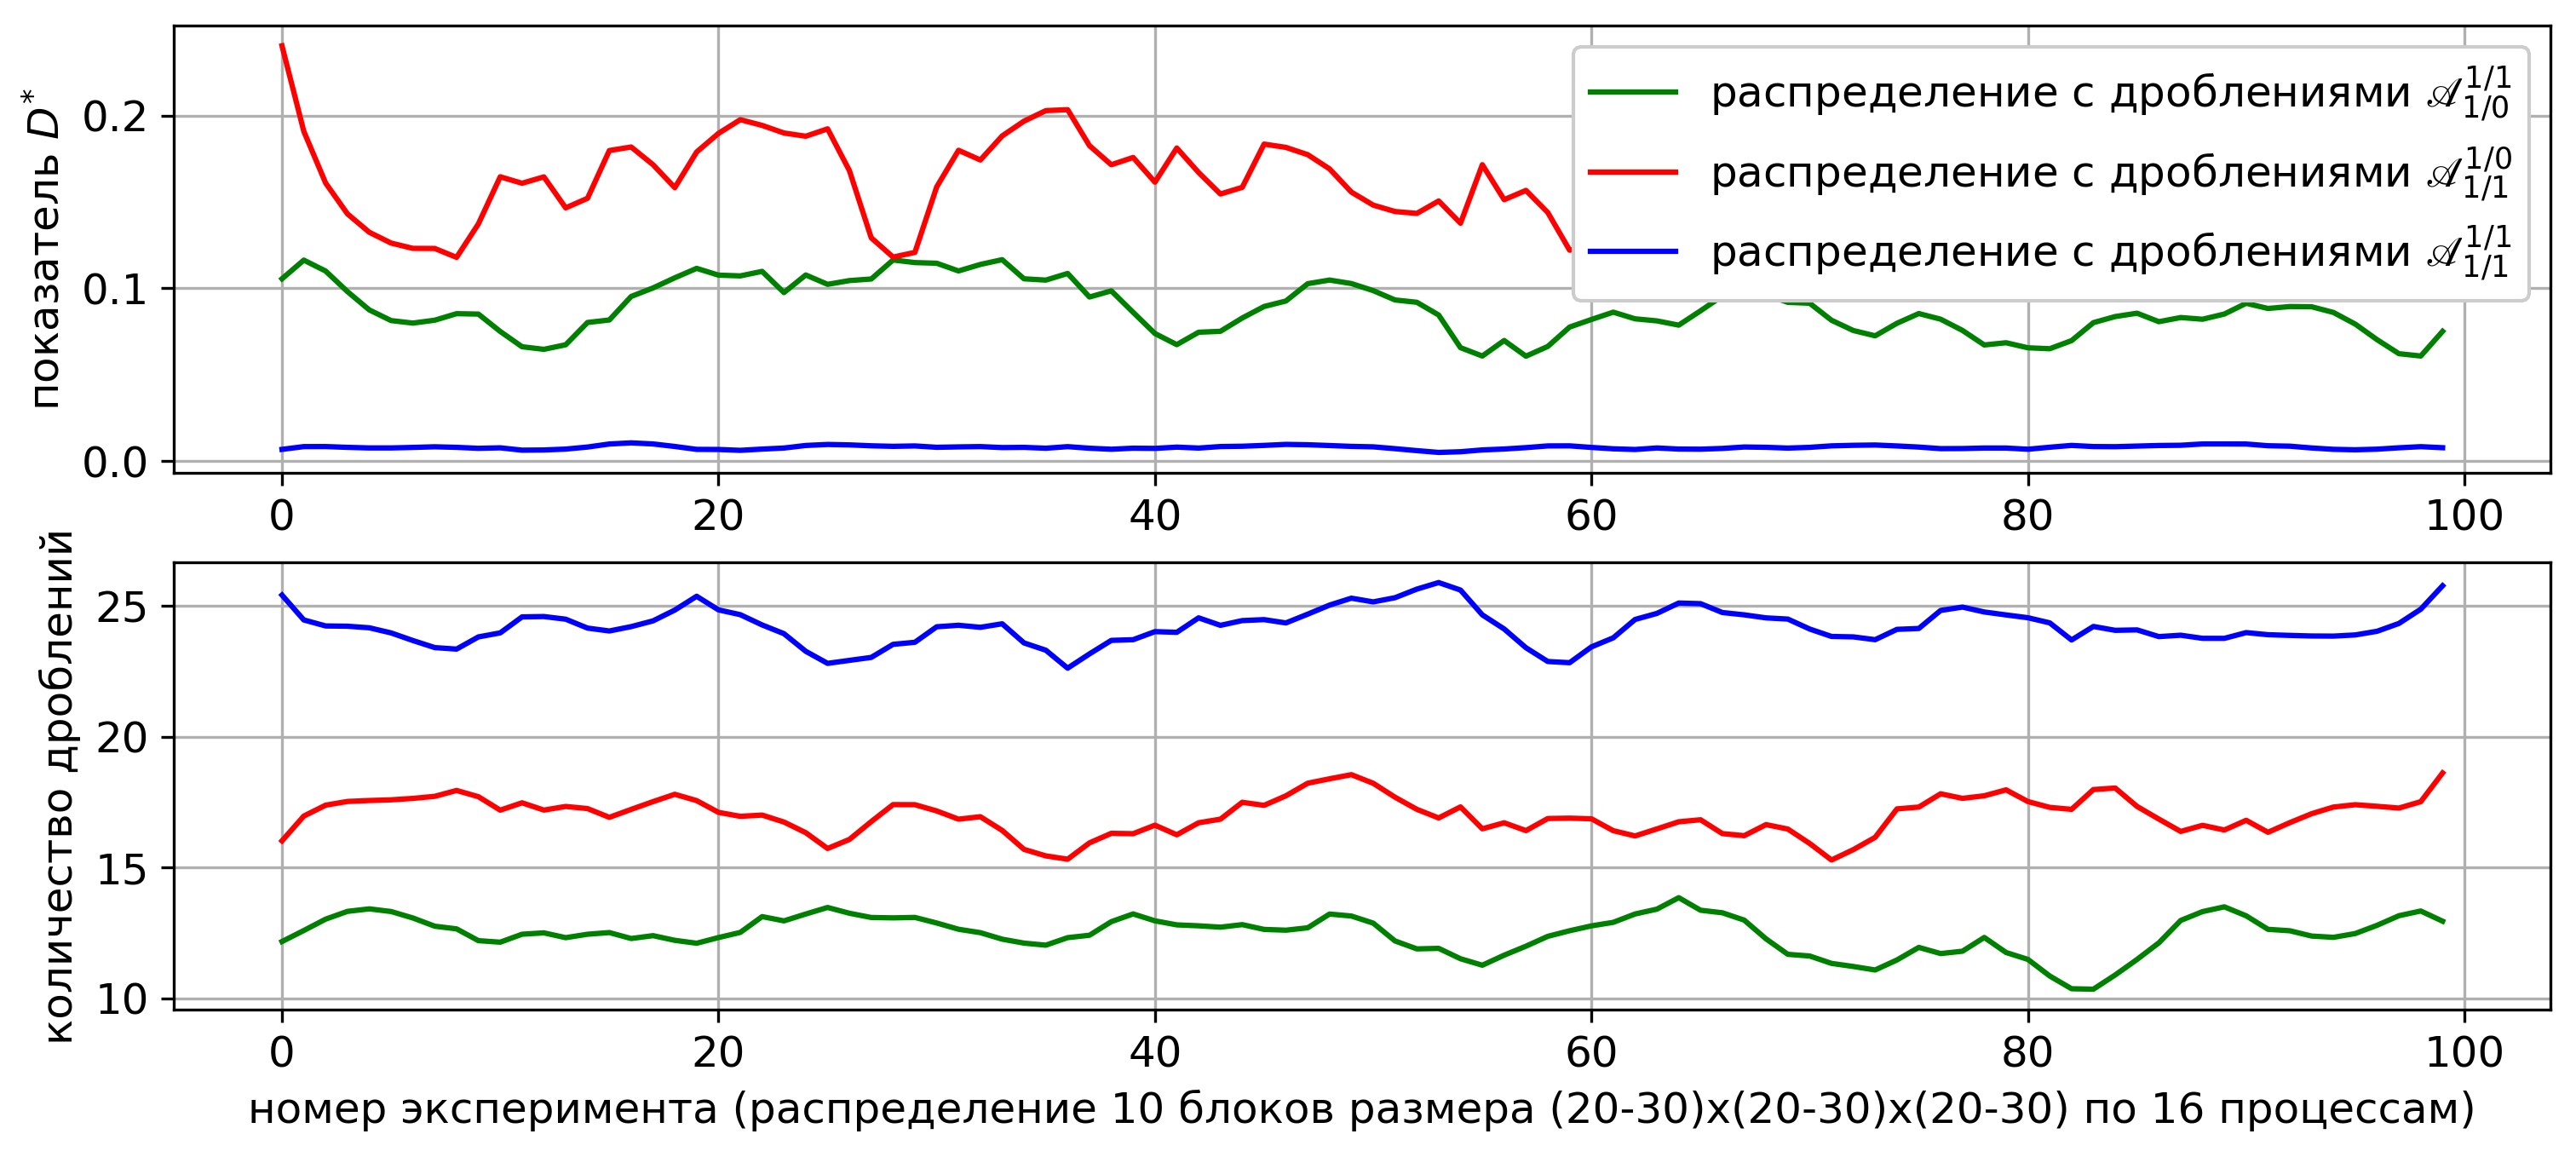
\includegraphics[width=1.0\textwidth]{fig/par_chart_distr_10_20_30_16.png}
\singlespacing
\captionstyle{center}\caption{Графики сравнения алгоримов $\mathscr{A}_{1/0}^{1/1}$, $\mathscr{A}_{1/1}^{1/0}$, $\mathscr{A}_{1/1}^{1/1}$ по показателю $D^{*}$ и количеству дроблений при распределении 10 случайных блоков по 16 партициям.}
\label{fig:par_chart_distr_10_20_30_16}
\end{figure}

\begin{figure}[!h]
\centering
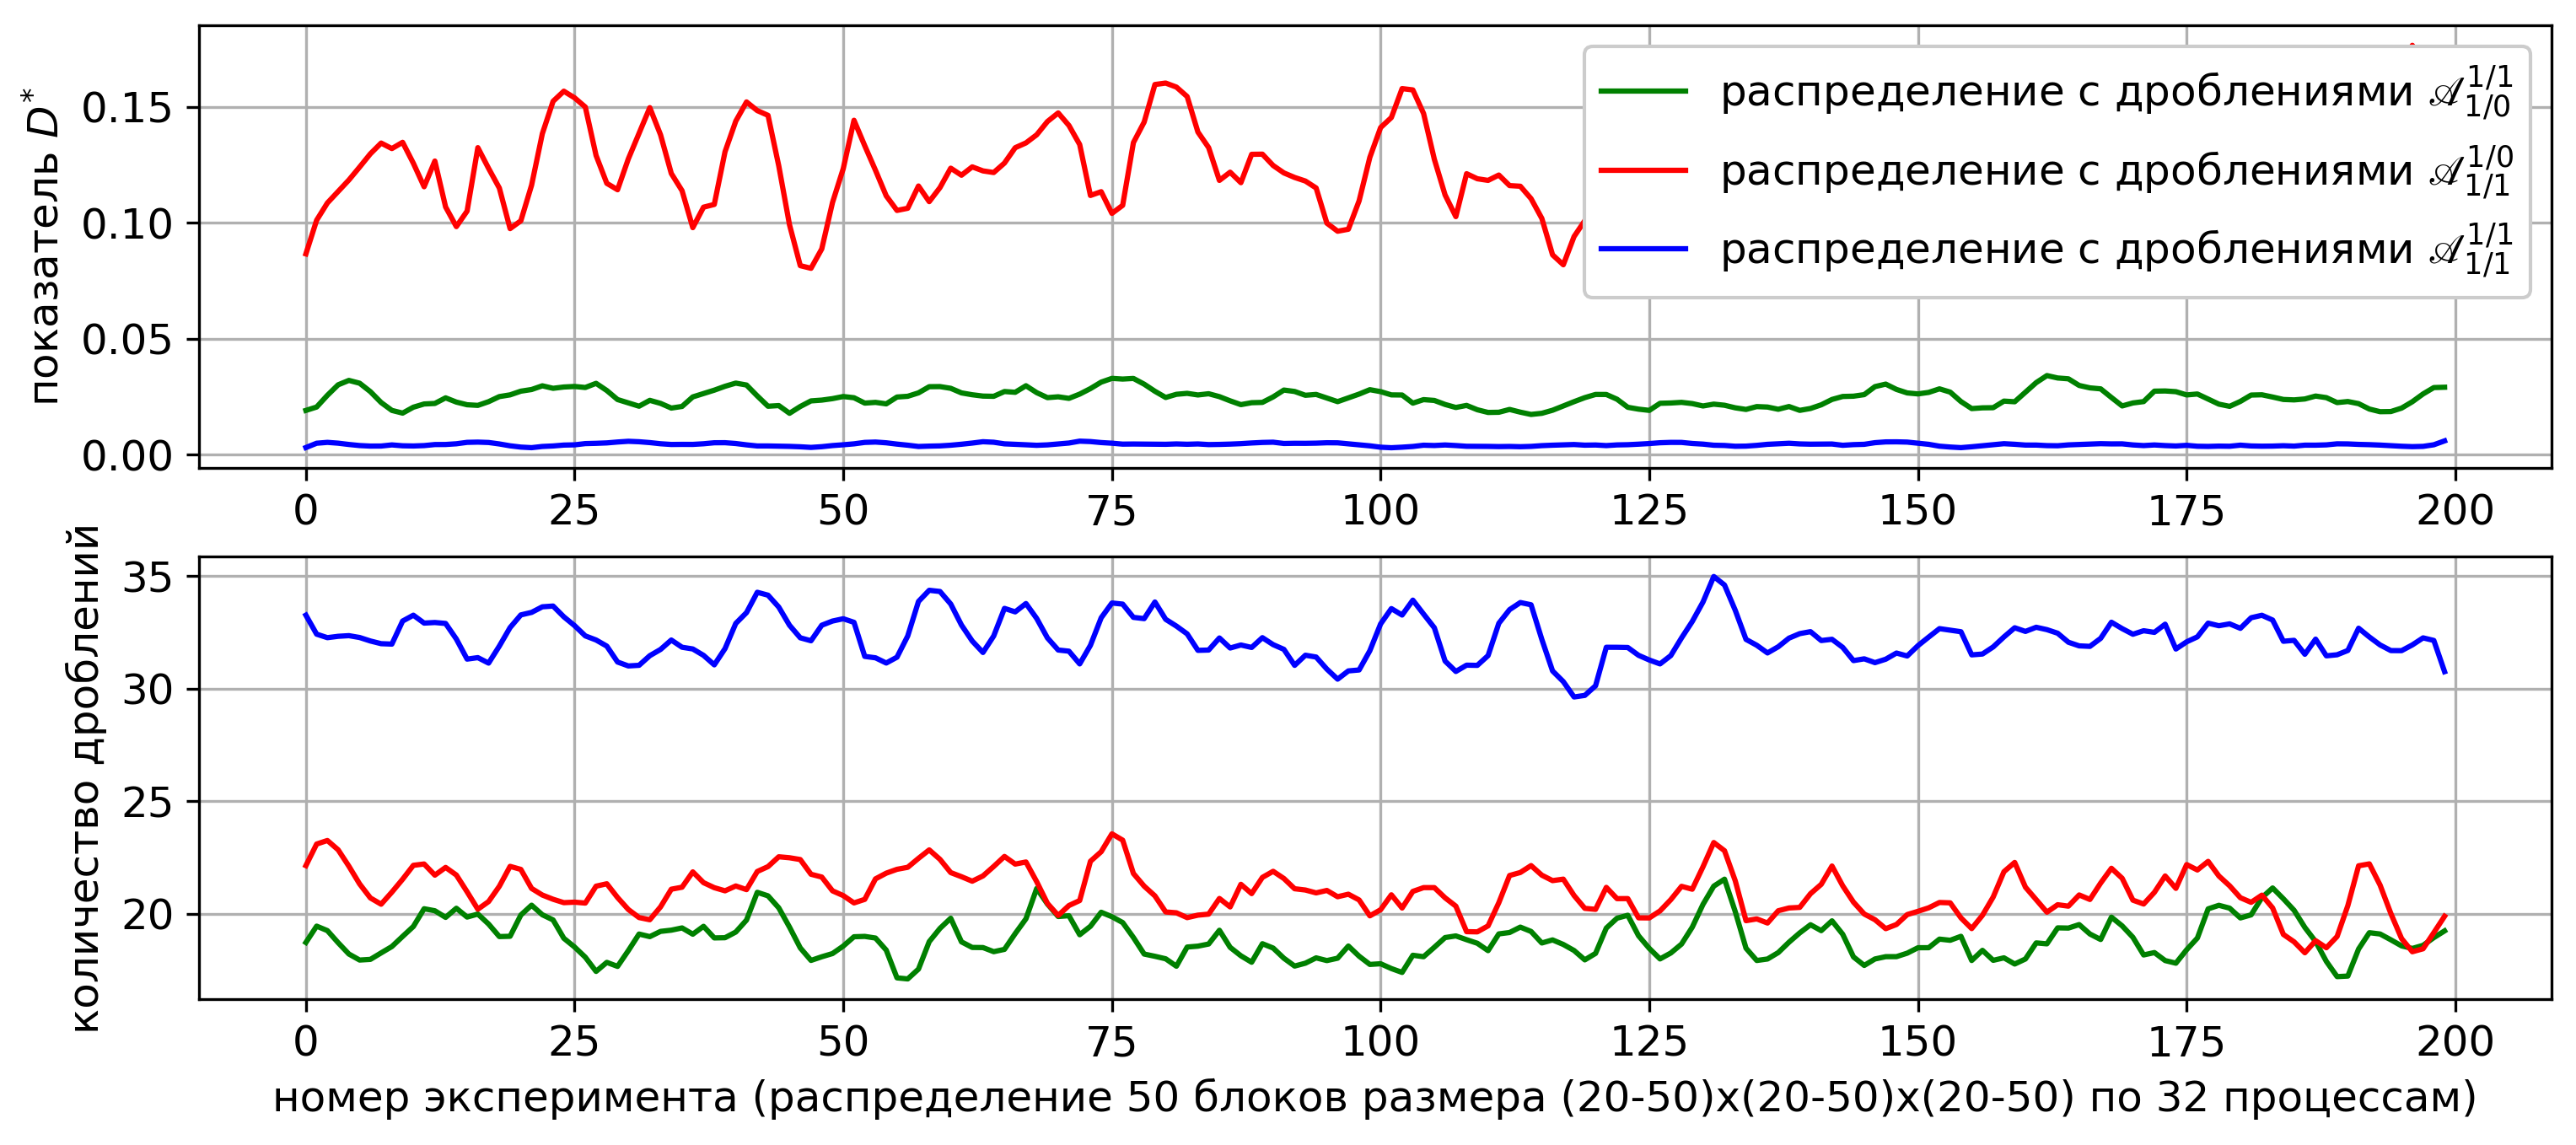
\includegraphics[width=1.0\textwidth]{fig/par_chart_distr_50_20_50_32.png}
\singlespacing
\captionstyle{center}\caption{Графики сравнения алгоримов $\mathscr{A}_{1/0}^{1/1}$, $\mathscr{A}_{1/1}^{1/0}$, $\mathscr{A}_{1/1}^{1/1}$ по показателю $D^{*}$ и количеству дроблений при распределении 50 случайных блоков по 32 партициям.}
\label{fig:par_chart_distr_50_20_50_32}
\end{figure}

\begin{figure}[!h]
\centering
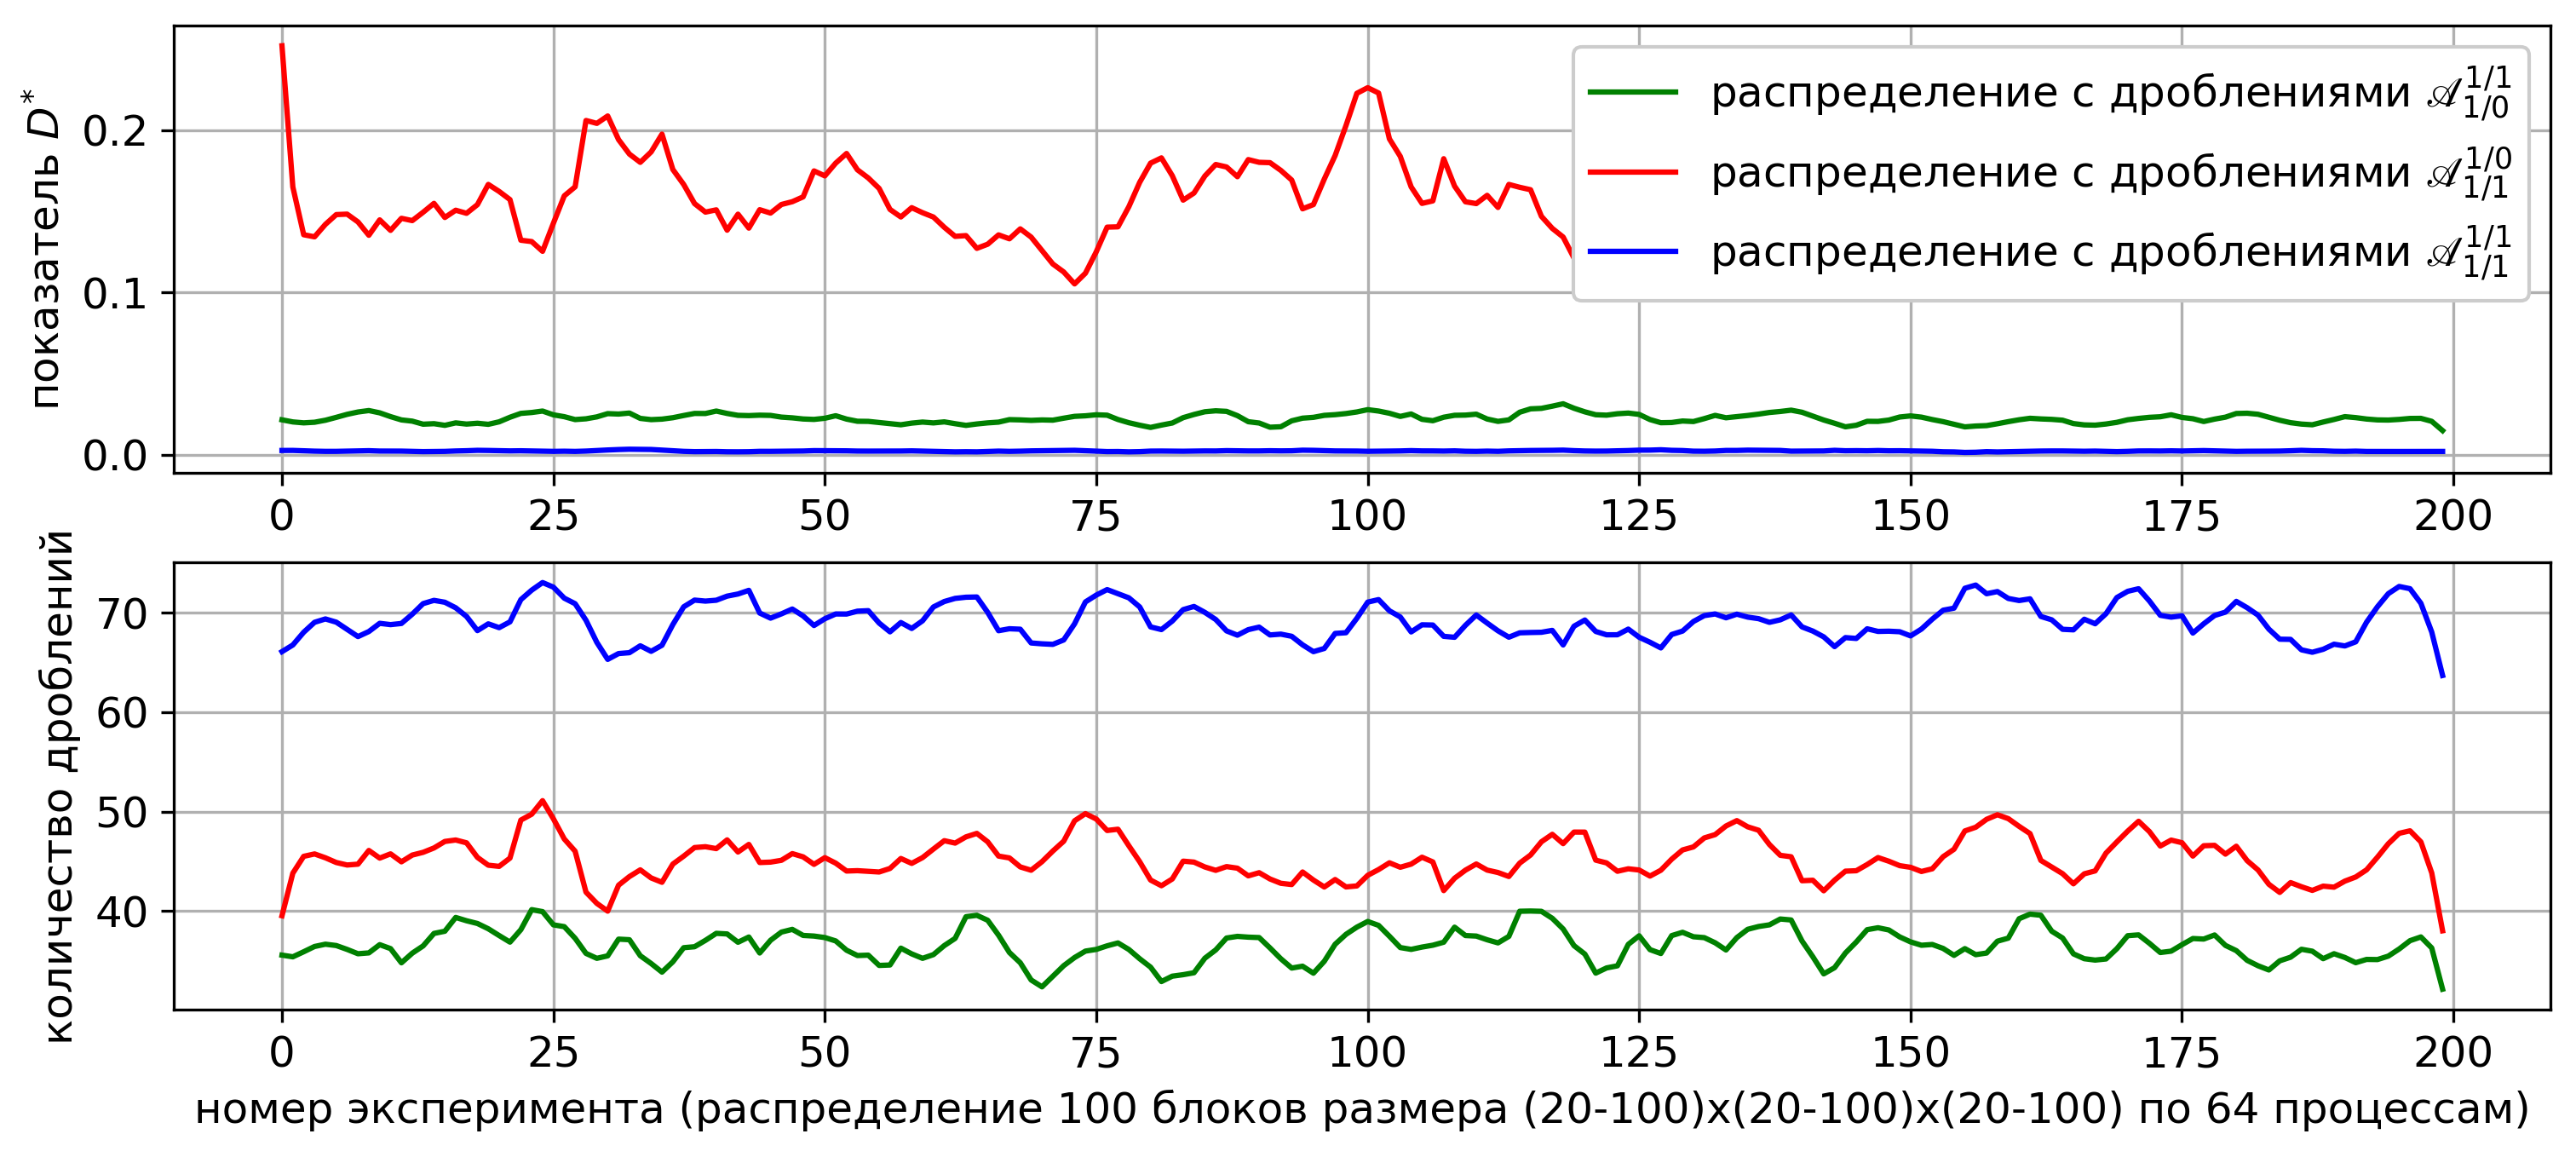
\includegraphics[width=1.0\textwidth]{fig/par_chart_distr_100_20_100_64.png}
\singlespacing
\captionstyle{center}\caption{Графики сравнения алгоримов $\mathscr{A}_{1/0}^{1/1}$, $\mathscr{A}_{1/1}^{1/0}$, $\mathscr{A}_{1/1}^{1/1}$ по показателю $D^{*}$ и количеству дроблений при распределении 100 случайных блоков по 64 партициям.}
\label{fig:par_chart_distr_100_20_100_64}
\end{figure}

Результаты работы алгоритмов $\mathscr{A}_{1/0}^{1/1}$, $\mathscr{A}_{1/1}^{1/0}$, $\mathscr{A}_{1/1}^{1/1}$ сравнивались между собой по двум характеристикам: показателю неравномерности рааспределения $D^{*}$ и количеству разрезов $\sigma$.
Сравнение выполнялось на наборах случайно сгенерированных блоков со сторонами заданного размера.
Рассматривались следующие примеры тестовых множеств блоков: распределение 10 блоков по сторонами размера 20-30 по 16 партициям (рис.~\ref{fig:par_chart_distr_10_20_30_16}), распределение 50 блоков со сторонами размера 20-50 по 32 партициям (рис.~\ref{fig:par_chart_distr_50_20_50_32}), распределение 100 блоков со сторонами размера 20-100 по 100 партициям (рис.~\ref{fig:par_chart_distr_100_20_100_64}).
Во всех случаях были приняты значения других параметров $\delta = 3$, $\Delta = 64$.

Из рис.~\ref{fig:par_chart_distr_10_20_30_16} -- \ref{fig:par_chart_distr_100_20_100_64} можно сделать следующие выводы.
Алгоритм $\mathscr{A}_{1/1}^{1/1}$ порождает наиболее равномерное распределение и приводит к наибольшему количеству дроблений, так как онн использует обе операции заполнения частями блоков (и снизу, и сверху).
Алгоритм $\mathscr{A}_{1/1}^{1/0}$ порождает наименее равномерное распределение, так как для заполнения сверху он использует только целые блоки, что приводит к росту ограничения $\tau$ в процессе работы алгоритма.
Алгоритм $\mathscr{A}_{1/0}^{1/1}$ является наиболее предпочтительным, так как по равномерности распределения он не сильно уступает алгоритму $\mathscr{A}_{1/1}^{1/1}$, а по количеству разрезов явялется наилучшим.

%---------------------------------------------------------------------------------------------------
% 4.3 - декомпозиция поверхностной сетки со сглаживанием границ

\subsection{Декомпозиция поверхностной неструктурированной расчетной сетки со сглаживанием границ доменов}

В этом разделе будем рассматривать подходы к декомпозиции неструктурированной поверхностной расчетной сетки с треугольными ячейками \cite{Rybakov2020Decomp}, на которой выполняются расчеты по моделированию ледообразования.
Для ускорения расчетов ячейки сетки разбиваются на отдельные домены, при этом нужно стремиться к уменьшению характеристик качества декомпозиции $D$, $L$, $I$.
В отличие от блочно-структурированных сеток у рассматриваемой неструктурированной сетки ячейки не объединяются в блоки, а являются независимыми объектами проведения расчетов.
Для неструктурированных поверхностных сеток будем считать, что вычислительная окрестность каждой ячейки будет влючать кроме нее самом только три смежные ячейки (граничащие с рассматривамой по каждому из трех ребер).

\subsubsection{Методы декомпозиции поверхностной \mbox{неструктурированной} расчетной сетки}\label{sec:par_decompsurf_methods}

Рассмотрим методы декомпозиции на примере тестовой трехмерной поверхностной сетки (wing), состоящей из ячеек-треугольников.
Сетка представляет собой профиль крыла летательного аппарата и содержит порядка $n = 2 \cdot 10^4$ ячеек.
Внешний вид тестовой расчетной сетки представлен на рис.~\ref{fig:text_2_decompsurf_wing_grid}.
Этот трехмерный профиль был сгенерирован из двумерного профиля NACA 0012 \cite{Naca0012}.

\begin{figure}[ht]
\centering
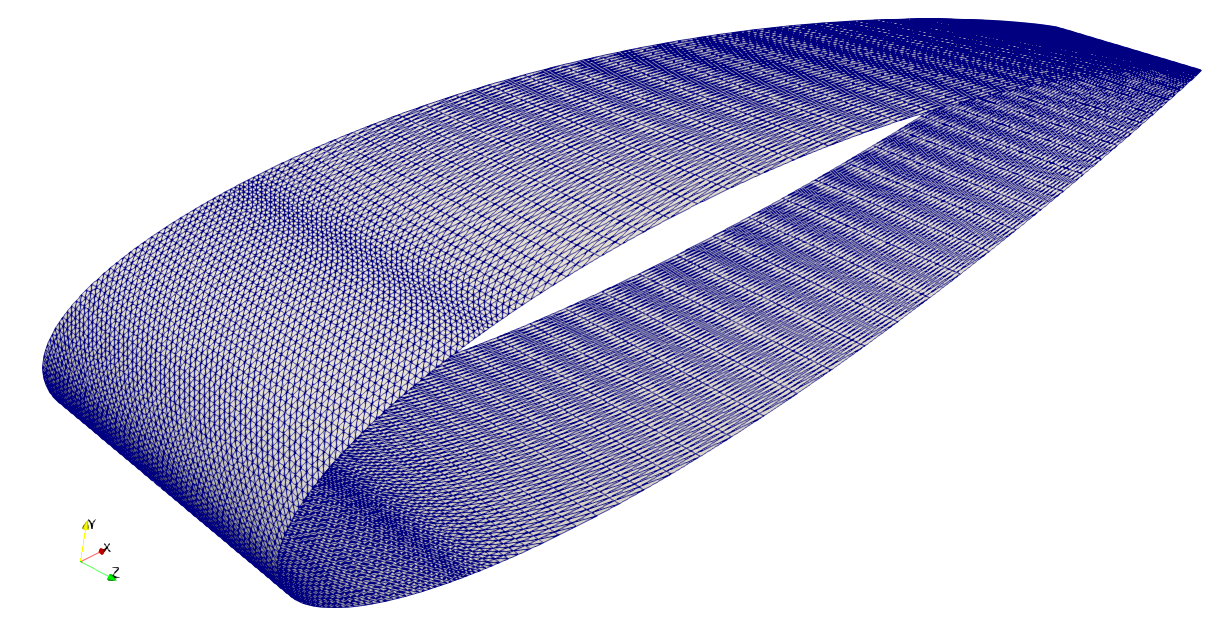
\includegraphics[width=0.45\textwidth]{fig/par_wing_grid.png}
\singlespacing
\captionstyle{center}\caption{Внешний вид расчетной сетки wing, используемой для тестирования алгоритмов декомпозиции.}
\label{fig:text_2_decompsurf_wing_grid}
\end{figure}

\begin{figure}[ht]
\centering
\begin{tabular}{ll}
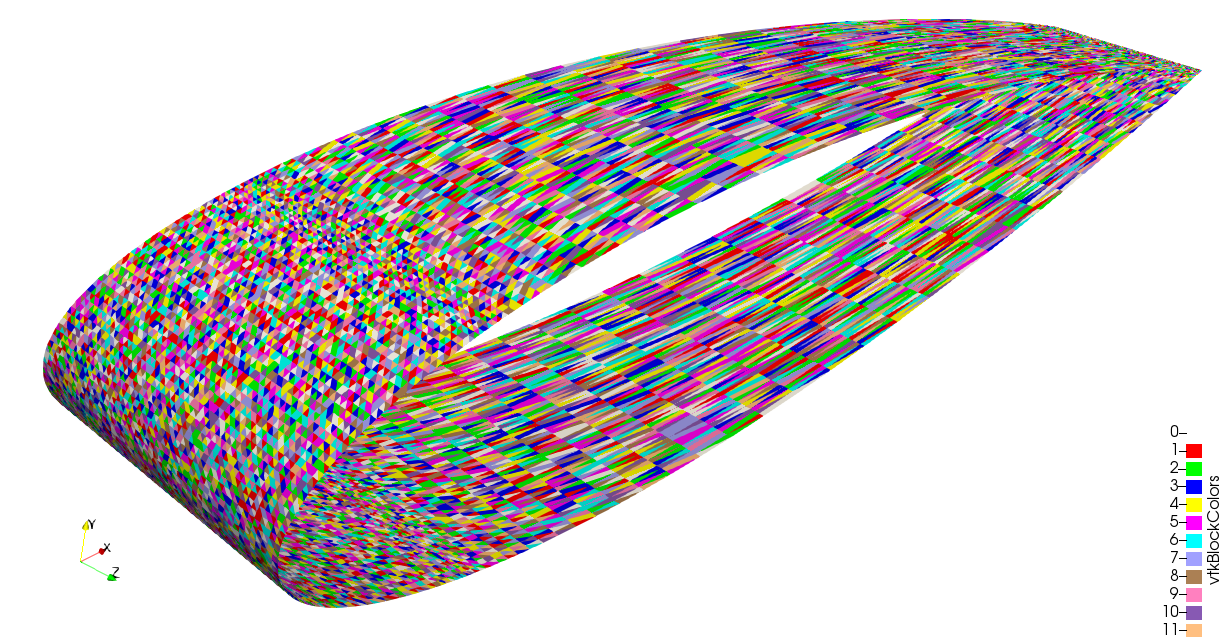
\includegraphics[width=0.4\textwidth]{fig/par_wing_random_32.png}
&
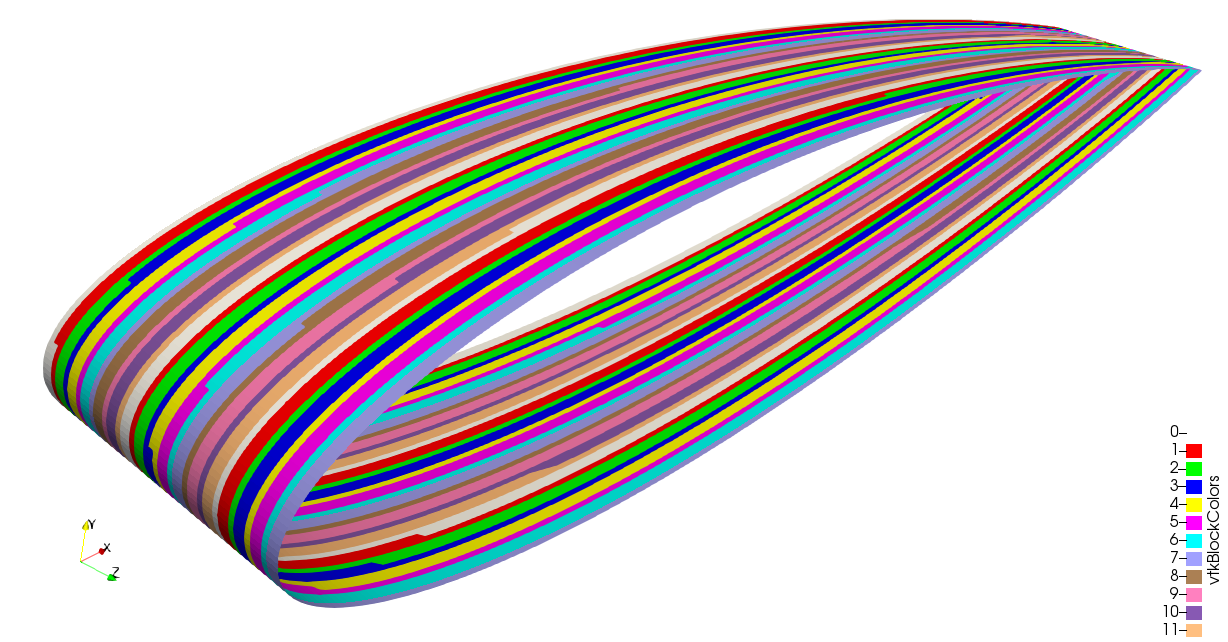
\includegraphics[width=0.4\textwidth]{fig/par_wing_linear_32.png}
\\
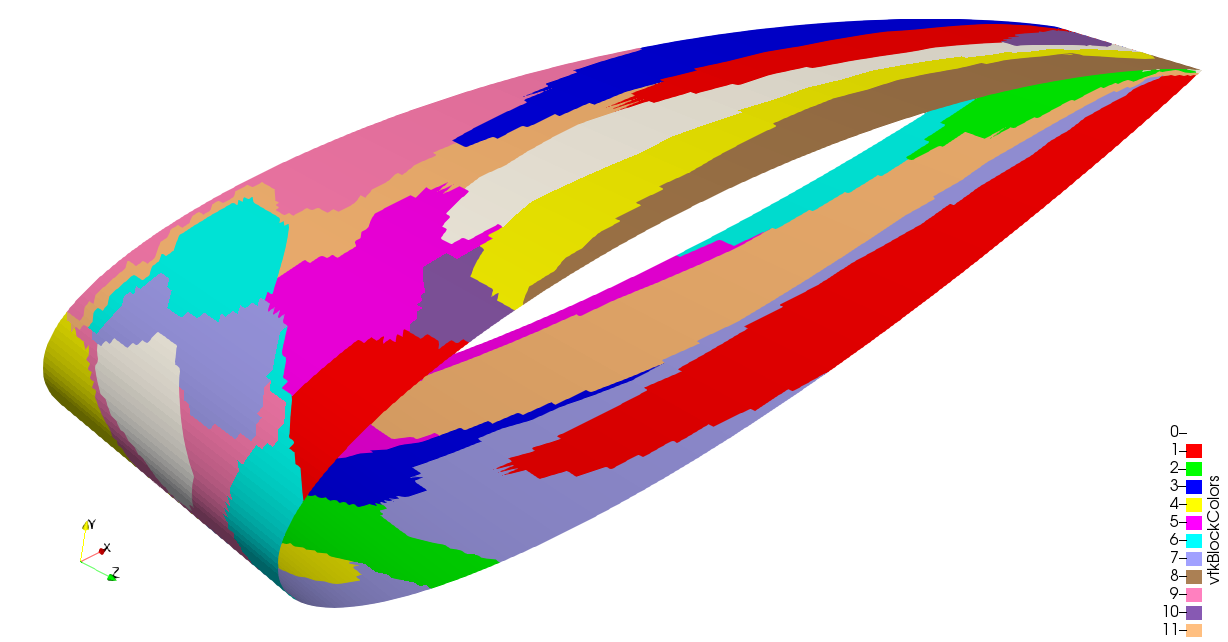
\includegraphics[width=0.4\textwidth]{fig/par_wing_rgrow_32.png}
&
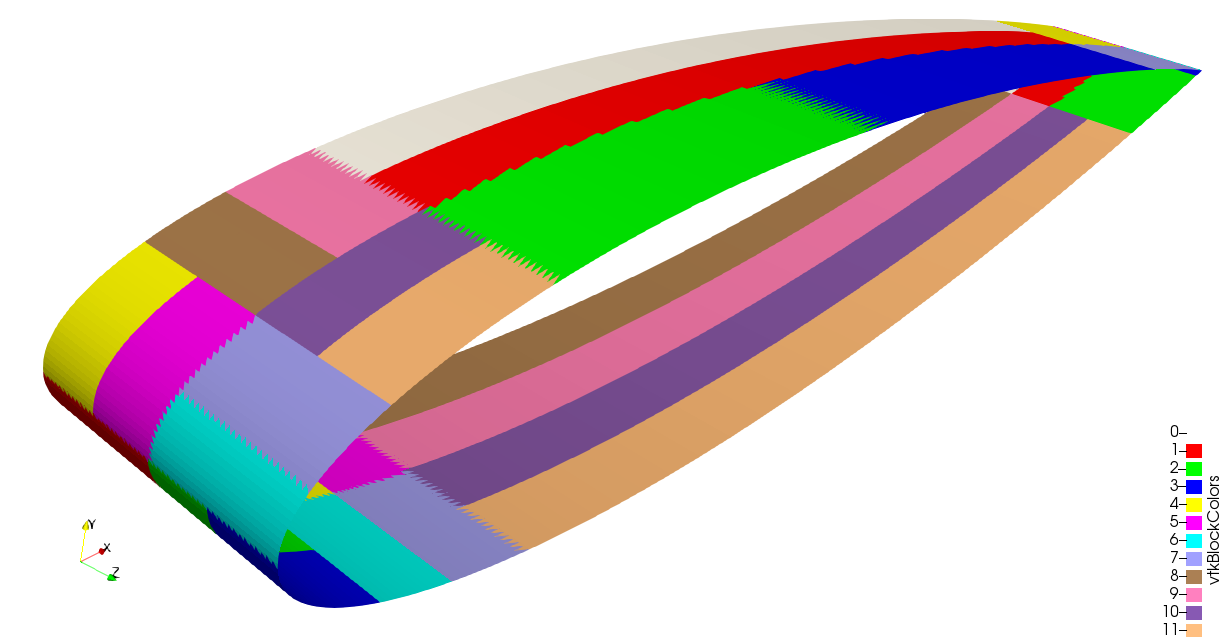
\includegraphics[width=0.4\textwidth]{fig/par_wing_hierarchical_32.png}
\end{tabular}
\singlespacing
\captionstyle{center}\caption{Результат декомпозиции расчетной сетки на 32 домена. Сверху вниз слева направо -- случайное распределение, линейное распределение, наращивание доменов и иерархическое дробление.}
\label{fig:text_2_decompsurf_4}
\end{figure}

В качестве первого и самого простого алгоритма декомпозиции рассмотрим алгоритм случайного распределения ячеек расчетной сетки по доменам.
Результат применения этого алгоритма к тестовой сетке показан на рис.~\ref{fig:text_2_decompsurf_4} сверху слева.
Алгоритм случайного распределения имеет достаточно низкое значение по критерию $D$, то есть распределение ячеек по доменам равномерное, однако при случайном распределении практически все ребра с высокой долей вероятности являются междоменными, что порождает огромный объем данных, которыми нужно обмениваться при синхронизации вычислений.
Также следует отменить, что при случайном распределении ячеек по доменам любые два домена оказываются соседними, граф связности доменов является полным.
Таким образом, каждый домен должен обмениваться данными со всеми остальными доменами по достаточно протяженным границам.
Также алгоритм становится совершенно непригодным, когда возникает необходимость создания теневых слоев глубиной больше единицы.

\begin{figure}[ht]
\centering
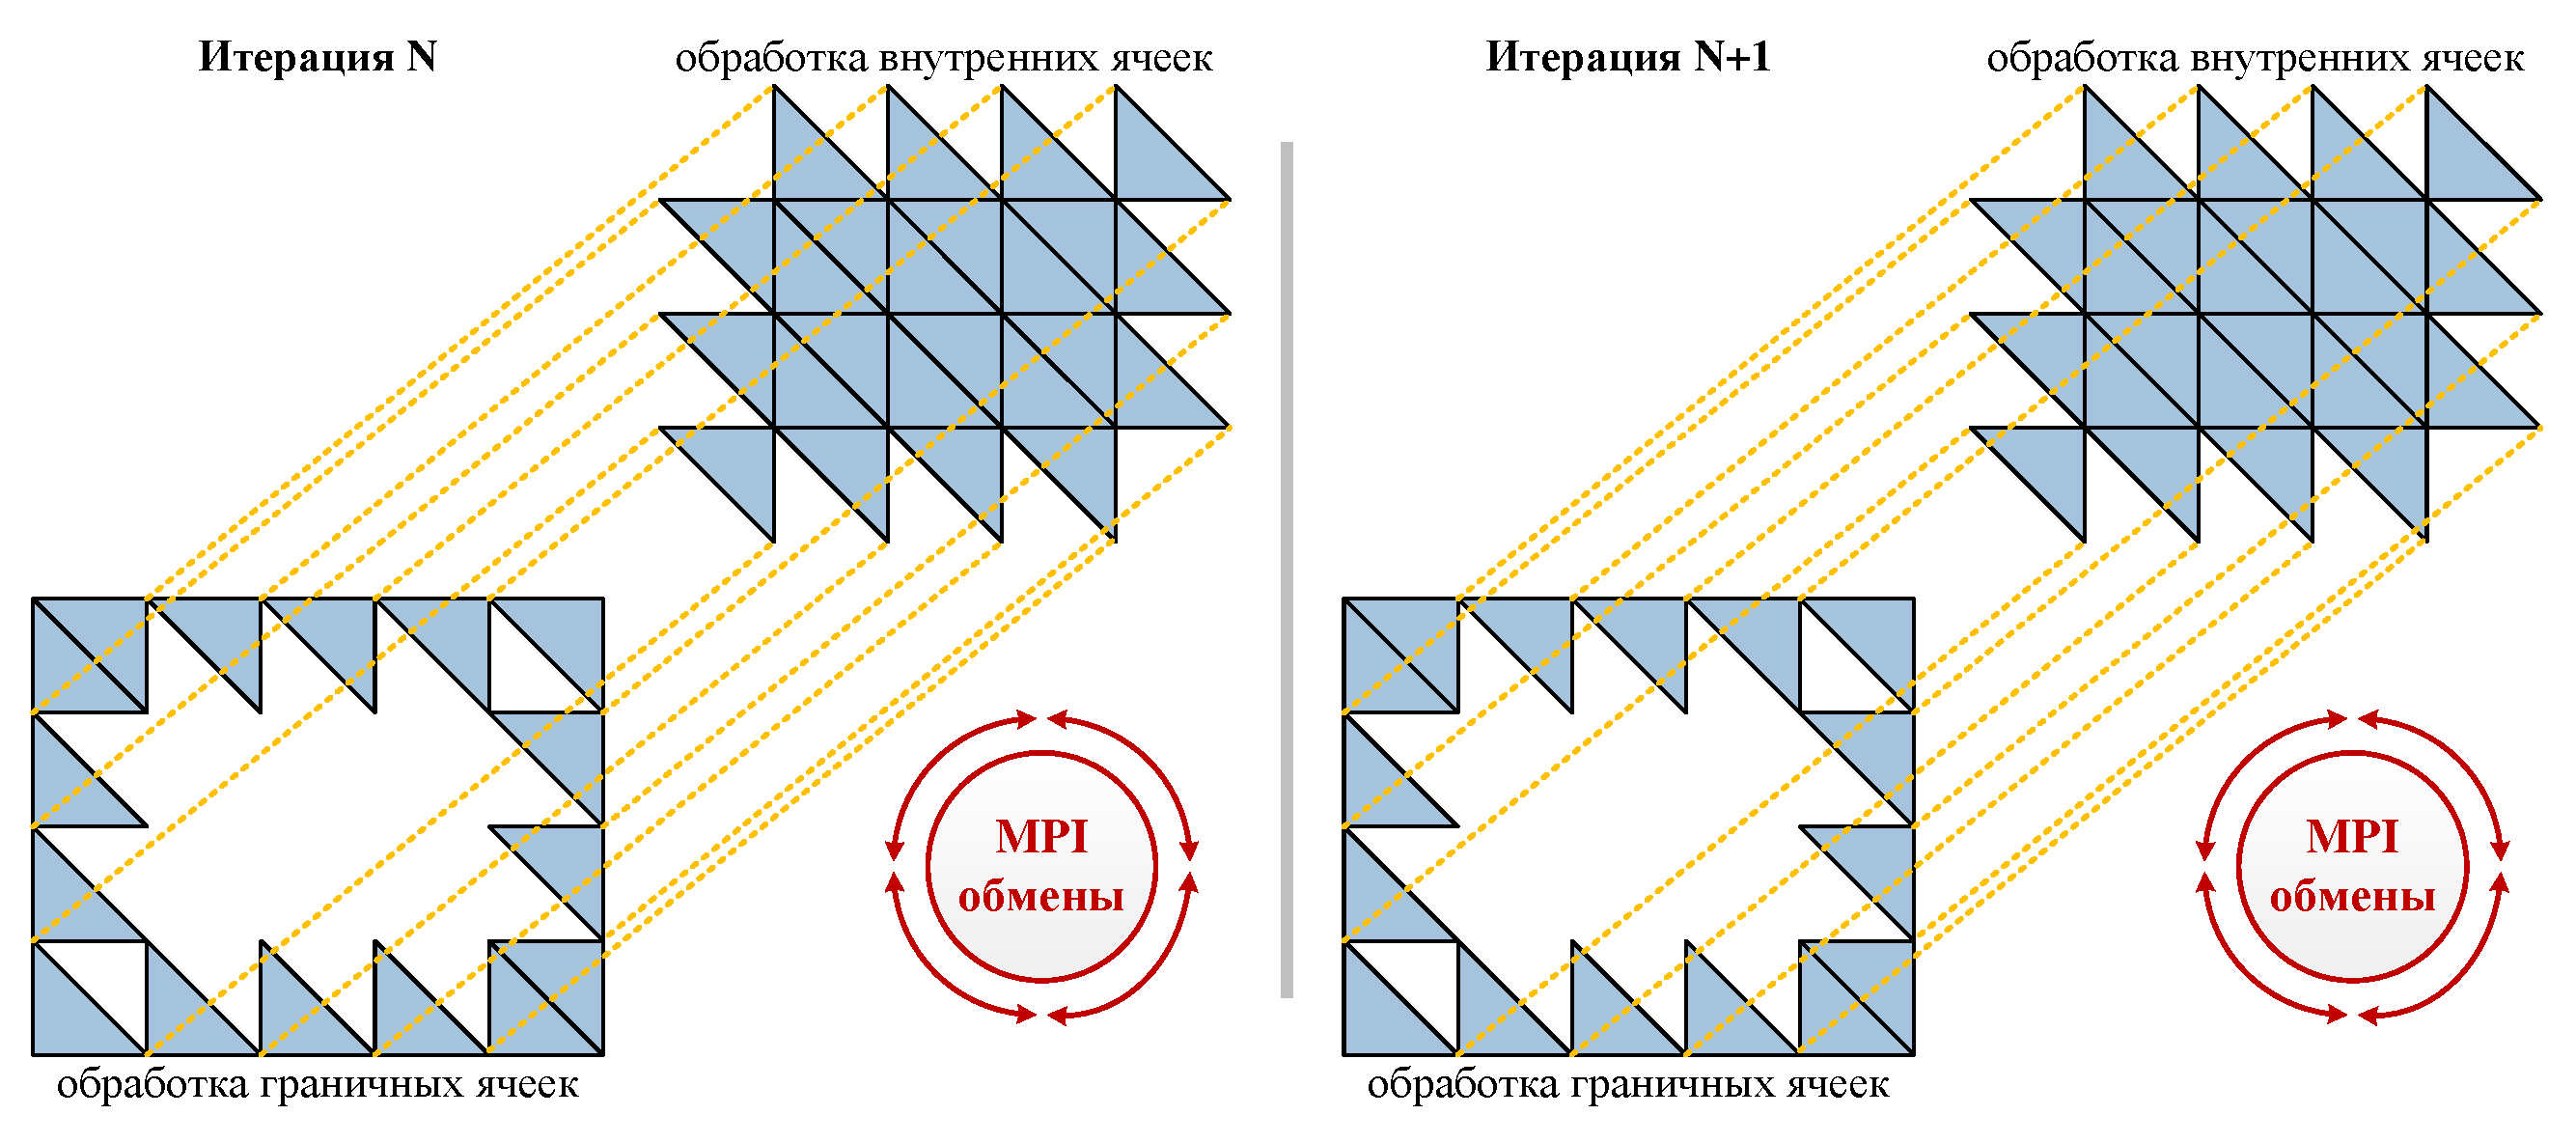
\includegraphics[width=0.8\textwidth]{fig/par_mpi_border_inner.pdf}
\singlespacing
\captionstyle{center}\caption{Сокрытие издержек на информационные обмены за вычислениями.}
\label{fig:text_2_decompsurf_wing_border_inner}
\end{figure}

На этом этапе упомянем механизм частичного сокрытия издержек на обмены данными за основными вычислениями.
Все ячейки каждого домена можно разделить на внутренние и граничные (аналогично внутренним и граничным ячейкам блока для блочно-структурированных сеток из раздела~\ref{sec:par_block_struct_mesh}).
Ценность внутренних ячеек состоит в том, что они не участвуют в обменах данными с соседними доменами, поэтому обработку внутренних ячеек для следующей итерации расчетов можно начинать, не дожидаясь завершения обменов данными на ребрах, составляющих границу между доменами (см. рис.~\ref{fig:text_2_decompsurf_wing_border_inner}).
Понятно, что такой подход неприменим при использовании случайного распределения ячеек по доменам, так как в большинстве случаев множества внутренних ячеек доменов оказываются практически пустыми.

Рассмотрим семейство алгоритмов декомпозиции, в которых учитываются только индексы распределяемых ячеек и никак не учитываются другие их данные.
Под индексом понимается номер ячейки в общем массиве ячеек расчетной сетки.
Уже по этому факту становится понятно, что такие алгоритмы не могут претендовать на высокое качество, так как их результат существенным образом зависит просто от порядка хранения данных расчетной сетки.
Самым простым из алгоритмов этого класса является алгоритм линейного распределения ячеек по доменам.
Так как в каждый домен в среднем должно войти по $\frac{n}{k}$ ячеек, где $n$ -- общее количество ячеек сетки, $k$ -- количество доменов (для простоты не будем обращать внимание на то, что это число может быть нецелым), то можно ячейки с номерами из диапазона $[0, \frac{n}{k} - 1]$ отнести к первому домену, ячейки с номерами $[\frac{n}{k}, \frac{2n}{k} - 1]$ ко второму домену и так далее.
При такой декомпозиции, конечно, можно добиться равномерного распределения ячеек по доменам, однако значения характеристик $L$ и $I$ в общем случае предугадать невозможно.
Например, на рассматриваемой тестовой сетке видно, что деление на домены вдоль профиля крыла (как это показано на рис.~\ref{fig:text_2_decompsurf_4} сверху справа) порождает очень длинные границы между соседними доменами.
Было бы гораздо эффективнее производить деление сетки поперек профиля.

В общем случае ячейки с непрерывным диапазоном индексов не обязаны составлять не то что компактные домены с границами небольшой протяженности, а вообще могут порождать несвязные домены, с изолированными ячейками, выколотыми ячейками и другими дефектами.
Применение таких алгоритмов оправдано только при обладании некоторой априорной информацией о структуре расчетной сетки (например, если известно, что сетка на самом деле является блочно-структурированной, в которой отдельные блоки соответствуют непрерывным диапазонам индексов ячеек).

Большой класс алгоритмов формируется из так называемых алгоритмов наращивания доменов.
В основе этих алгоритмов лежит следующий принцип: вначале выбирается ячейка (или несколько ячеек), от которой (или которых) далее производится наращивание одного или нескольких доменов путем последовательного добавления соседних ячеек.
В рамках этого класса алгоритмов при последовательном создании доменов размера $\frac{n}{k}$ получим алгоритм Фархата, результатом которого являются домены с очень протяженными границами \cite{Farhat1988Decomp}.
При использовании одновременного роста сразу нескольких доменов от случайных ячеек расчетной сетки получаем алгоритм пузырькового роста \cite{Preis1997Decomp}, который требуется запускать на расчетной сетке итерационно несколько раз для получения приемлемых характеристик качества декомпозиции.
При этом алгоритм пузырькового роста не гарантирует сбалансированного разбиения ячеек сетки по доменам (для достижения этого необходимо производить дополнительную коррекцию).
Также следует отметить инкрементальный алгоритм декомпозиции \cite{Yakobovsky2005Decomp}, особенностью которого является возможность освобождения части ячеек, уже распределенных по доменам, с последующим повторением роста доменов.

Мы рассматриваем простой алгоритм наращивания доменов, в котором все домены наращиваются одновременно, начиная с некоторых случайно выбранных ячеек сетки.
При этом поддерживается связность доменов -- если в какой-то момент домену больше некуда расти, то он прекращает свой рост и больше не расширяется.
Таким образом, возможна генерация крайне неравномерных по количеству ячеек доменов.
Пример результата применения этого алгоритма приведен на рис.~\ref{fig:text_2_decompsurf_4} снизу слева.

Кроме приведенных алгоритмов существует множество подходов к декомпозиции расчетных сеток, среди них алгоритмы, основанные на методе спектральной бисекции \cite{Urschel2014Decomp}, диффузионные и генетические алгоритмы \cite{Zhao2019Decomp}, иерархические алгоритмы \cite{Kapyris1998Decomp} и другие.
Наиболее полный обзор различных алгоритмов декомпозиции расчетных сеток можно найти в \cite{Golovchenko2020Decomp} и \cite{Zheleznyakova2017Decomp}.

Далее рассмотрим два алгоритма декомпозиции поверхностной неструктурированной расчетной сетки, с помощью которых можно добиться достаточно низких показателей характеристик распределения $D$, $L$, $I$.

%\subsubsection{Алгоритм декомпозиции с помощью иерархического деления доменов}\label{sec:text_2_decompsurf_hierarchical}

В работе \cite{Golovchenko2020Decomp} приведено описание параллельного алгоритма геометрической декомпозиции сеточных данных.
Во время работы этого алгоритма происходит последовательное деление текущего домена пополам с помощью сечения плоскостью.
На рис.~\ref{fig:text_2_decompsurf_hierarchical} продемонстрирована схема, по которой изначальный головной домен $h$ делится на пару доменов $hl$ и $hr$, каждый из которых делится далее пополам и так далее на любое количество доменов, равное степени двойки.

\begin{figure}[ht]
\centering
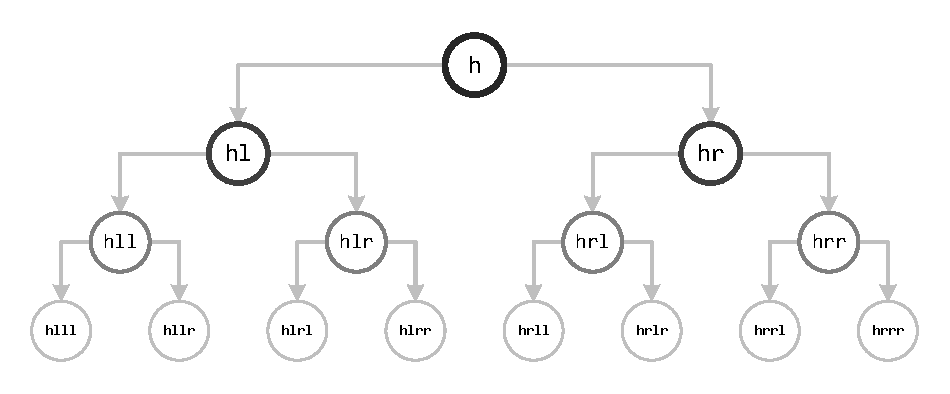
\includegraphics[width=0.8\textwidth]{fig/par_hierarchical.pdf}
\singlespacing
\captionstyle{center}\caption{Иллюстрация иерархического трехуровневого разделения головного домена.}
\label{fig:text_2_decompsurf_hierarchical}
\end{figure}

Этот алгоритм можно расширить, введя в него произвольные критерии разбиения текущего домена на пару более мелких доменов.
Вначале рассмотрим схему простого деления домена пополам с использованием произвольного признака, по которому производится деление (см. рис.~\ref{fig:text_2_decompsurf_split}).

\begin{figure}[ht]
\centering
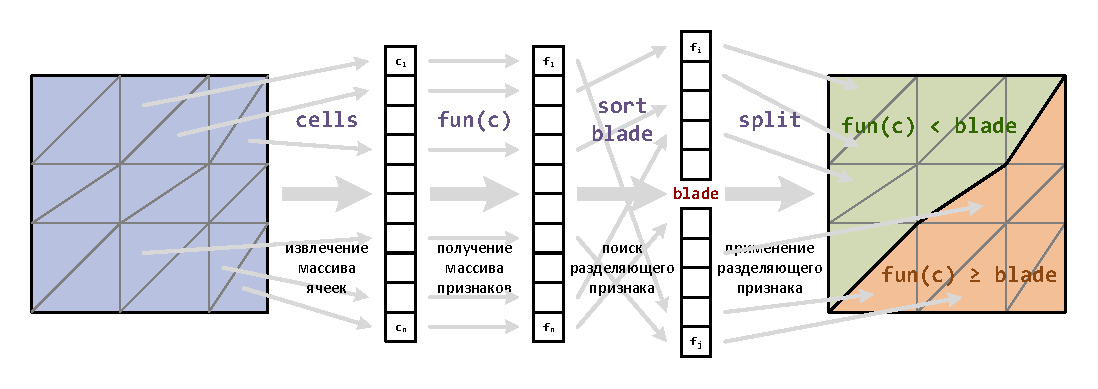
\includegraphics[width=1.0\textwidth]{fig/par_split.pdf}
\singlespacing
\captionstyle{center}\caption{Схема выполнения разделения домена пополам по заданному признаку fun.}
\label{fig:text_2_decompsurf_split}
\end{figure}

Пусть задан массив ячеек домена $C$ и произвольная функция извлечения признака из ячейки $fun$.
Первым шагом является вычисление массива признаков для всех ячеек.
После этого половина массива с меньшими значениями признака формирует один дочерний домен, а вторая половина с большими значениями признаков формирует второй дочерний домен.

После разделения домена на два более мелких домена можно вычислить параметр, отражающий эффективность разбиения.
В качестве такого параметра предлагается использовать длину границы между двумя образованными новыми доменами.
Таким образом, критерий разбиения зависит от функции вычисления признака $fun$.
В свою очередь это означает, что при выполнении разбиения не обязательно ограничиваться одной функцией вычисления признака, вместо этого можно подать список функций, для каждой функции вычислитель показатель качества разбиения и в результате остановиться на той функции вычисления признака, которая приводит к наиболее эффективному разбиению.
Если в качестве функций вычисления признака ячейки использовать просто извлечение трех координат центров ячеек, то мы получим в чистом виде алгоритм геометрической декомпозиции сетки с выбором для дробления наиболее протяженного размера по одной из координат.
Результат применения этого алгоритма показан на рис.~\ref{fig:text_2_decompsurf_4} снизу справа.

\begin{figure}[H]
\centering
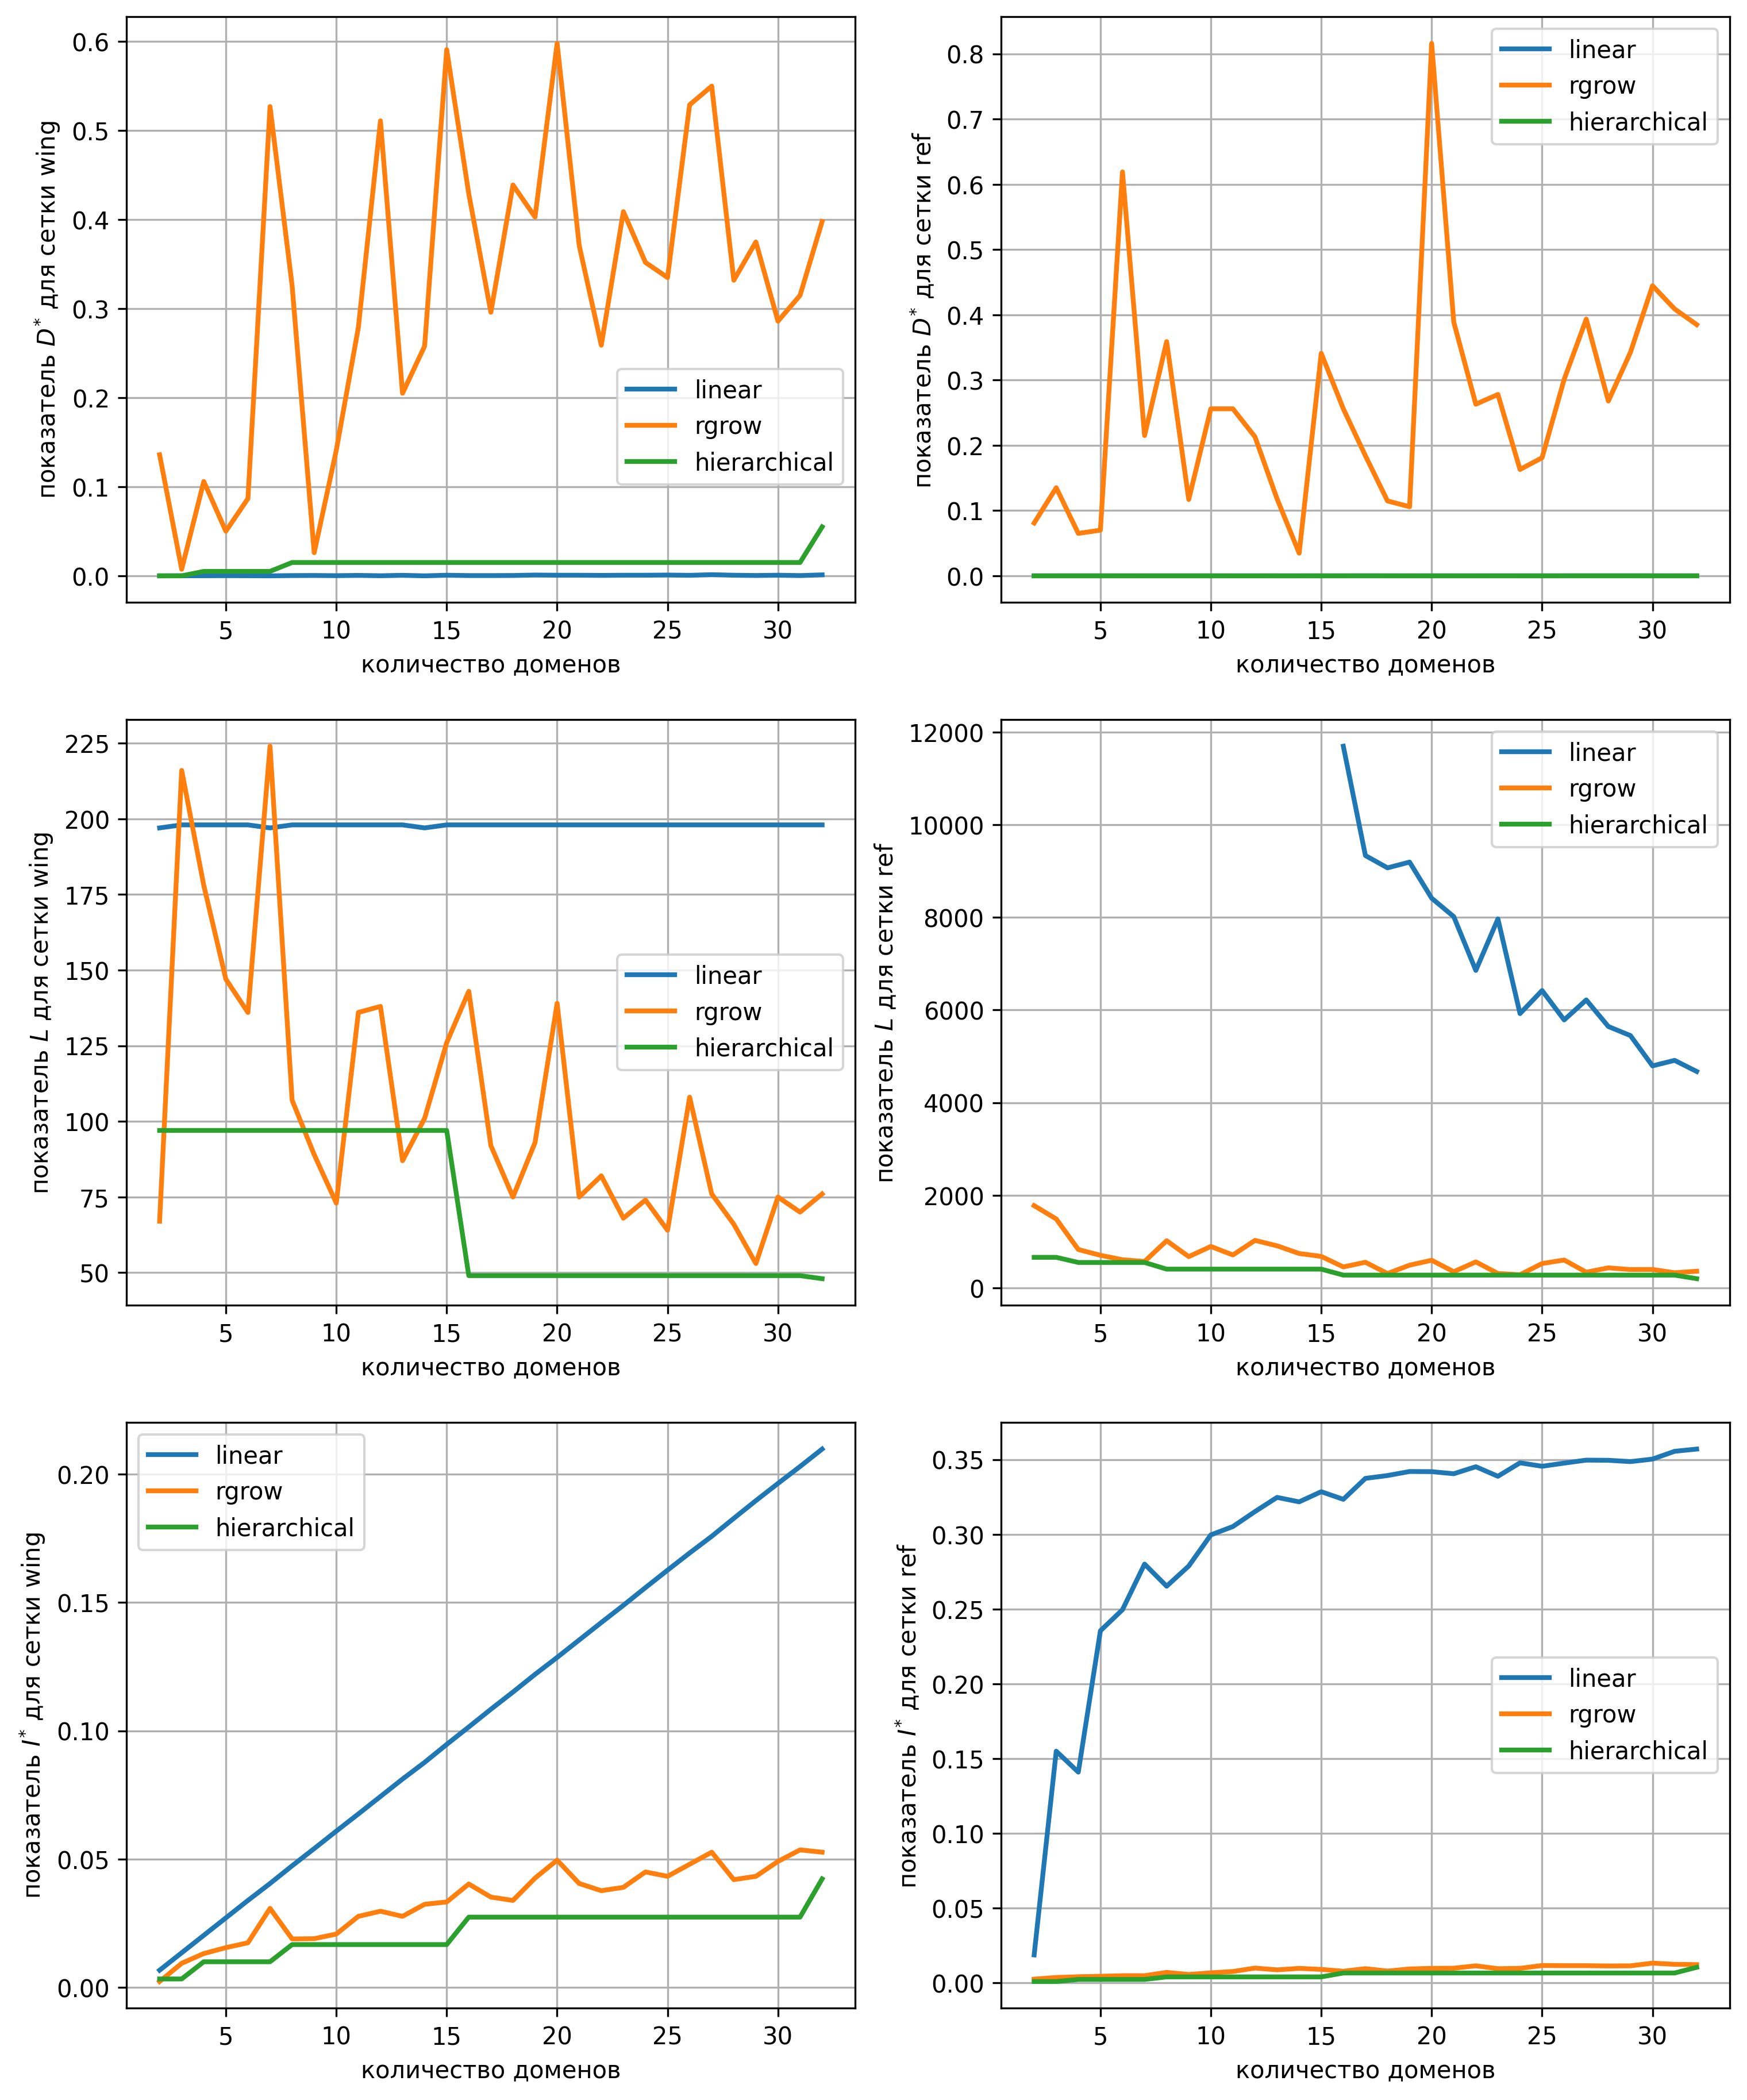
\includegraphics[width=1.0\textwidth]{fig/par_decompsurf_qual.png}
\singlespacing
\captionstyle{center}\caption{Графики показателей $D^{*}$, $L$, $I^{*}$ для сеток wing и ref.}
\label{fig:text_2_decompsurf_qual}
\end{figure}

На рис.~\ref{fig:text_2_decompsurf_qual} представлены графики характеристик $D^{*}$, $L$, $I^{*}$, вычисленные во время применения различных алгоритмов декомпозиции поверхностной расчетной сетки на разное количество доменов от 2 до 32.

Для эксперимента использовались две сетки.
Первая сетка -- wing, представленная на рис.~\ref{fig:text_2_decompsurf_wing_grid}.
Вторая сетка -- ref -- более приближена к реальной геометрии летательного аппарата и содержит порядка $n = 4 \cdot 10^5$ ячеек.
На графиках введены следующие краткие названия алгоритмов: linear -- линейное разделение ячеек между доменами по индексу, rgrow -- алгоритм наращивания доменов от случайных ячеек, hierarchical -- иерархическое деление доменов пополам по одной из трех координат.

При этом отметим, что при использовании алгоритма rgrow умышленно использовалась только одна итерации наращивания, для демонстрации того, насколько неравномерным может быть распределение размеров доменов при случайном выборе инициирующих ячеек (из рисунков видно, что значение параметра $D^{*}$ достигает значениий 0,6 и 0,8 для сеток wing и ref соответственно).

Из приведенных графиков можно сделать вывод, что из представленных алгоритмов иерархическое деление доменов с выбором оптимального критерия деления из списка функций вычисления признаков ячеек является наиболее приемлемым по параметрам $D^{*}$, $L$, $I^{*}$, то есть с помощью этого алгоритма генерируется достаточно равномерное распределение ячеек по доменам при низкой общей доле междоменных ребер и малой протяженности границ между доменами.

% Наверное не надо его выделять.
%\subsubsection{Генетический алгоритм декомпозиции неструктурированной расчетной сетки}\label{sec:text_2_genetic}

Анализ графиков с рис.~\ref{fig:text_2_decompsurf_qual} позволяет сделать вывод, что алгоритм наращивания доменов является пригодным для практического применения с точки зрения характеристик $L$, $I$ и для повышения его эффективности необходимо добиться уменьшения показателя $D$.
Рассмотрим генетический подход к улучшению расположения инициирующих вершин в алгоритме наращивания доменов \cite{Rybakov2025GenDecomp}.

Генетические алгоритмы представляют собой природоподобные эвристические алгоритмы, с помощью которых можно искать решения оптимизационных задач с большим количеством параметров \cite{Chahar2021Gen}.
В процессе применения генетического алгоритма моделируется процесс создания, выживания и размножения популяции потенциально возможных решений поставленной проблемы в условиях сложно устроенной окружающей среды.
Работа генетического алгоритма начинается с создания стартовой популяции потенциальных решений проблемы, где каждое представлено отдельной особью, определяемой набором характеризующих ее генов (генотипом).
Для особи должна быть определена функция пригодности, которая является индикатором качества для решения поставленной задачи (вместо функции пригодности можно использовать штрафную функцию, которая наоборот является показателем непригодности). 
На каждой эпохе генетического алгоритма на основе текущей популяции создается следующая популяция, которая по ожиданиям в среднем должна быть более приспособлена к условиям окружающей среды.
Генетические алгоритмы широко применяются во многих областях, для решения задач с большим количеством параметров и ограничений.
Применение генетических алгоритмов не подразумевает отыскание оптимального решения, однако с их использованием можно быстро найти решение, которое является достаточно качественным в текущих условиях.
В частности генетические алгоритмы примеными в задаче декомпозиция графа \cite{Chaouche2023Graph,Li2020Graph}.

При использовании генетических алгоритмов важно различать понятие генотипа и особи.
Генотип -- это набор генов, некий код, который кодирует механизм создание особи.
Особь -- сформированный на основе генотипа индивид, который обладает определенными свойствами и характеристиками, и для которого может быть вычислена функция пригодности или штрафная функция.
Зачастую при использовании генетических алгоритмов различие между генотипом и особью стирается, и вместо генотипа используется просто явное представление особи.
Так в работе \cite{Chaouche2023Graph} при декомпозиции графа в генотипе кодируется каждое ребро рассматриваемого графа, а в работе \cite{Li2020Graph} генотип представляет собой точное соотнесение каждой вершины графа и результирующего домена.
Использование генотипа в роли особи в генетических алгоритмах приводит к существенному замедлению сходимости, что снижает ценность использования этих алгоритмов.
К тому же применение механизмов скрещивания и мутаций к особям вместо генотипов также вызывает сомнение с точки зрения корректности таких операций.
Рассмотрим подход, в котором в качестве генотипа используется максимально короткий код, по которому может быть быстро построена особь.

Рассмотрим алгоритм декомпозиции дуального графа произвольной расчетной сетки на $k$ доменов.
Количество вершин в графе равно $n$.
При этом рассматриваемый дуальный граф задан структурами \texttt{inc} и \texttt{es}.
В структуре \texttt{inc} хранятся соседи каждой вершины графа: \texttt{inc[i]} -- вектор номеров всех вершин, смежных $i$-й вершине.
Структура \texttt{es} -- множество ребер графа.
В качестве особи будем рассматривать вектор \texttt{domains} длины $n$, в котором \texttt{domains[i]} -- номер домена, к которому отнесена $i$-ая вершина графа.
В качестве штрафной функции особи будем использовать функцию $Q = \delta D + \lambda L$.

Ключевым элементом генетического алгоритма является понятие генотипа и процесс формирования особи на основе генотипа.
В качестве генотипа будем использовать вектор \texttt{genotype} длины $k$, задающий $k$ номеров вершин дуального графа, которые будем называть инициирующими, или опорными вершинами.
При инициализации каждую опорную вершину \texttt{genotype[i]} будем принудительно относить к $i$-му домену.
При построении особи на основе генотипа будем распределять вершины между доменами с помощью простого алгоритма пузырькового роста доменов, одновременно обходя граф в ширину начиная с опорных вершин.
%Программный код процедуры распределения вершин между доменами можно видеть на листинге~\ref{lst:text_2_gen_alg}.

%\begin{singlespace}
%\begin{lstlisting}[caption={Простая декомпозиция, используемая в генетическом алгоритме.},label={lst:text_2_gen_alg}]
%deque<size_t> q;
%
%for (auto i { 0 }; i < k; ++i)
%{
%    domains[genotype[i]] = i;
%    q.push_back(genotype[i]);
%}
%
%while (!q.empty())
%{
%    auto node { q.front() };
%    auto domain { domains[node] };
%    q.pop_front();
%
%    for (auto ngh : inc[node])
%    {
%        if (domains[ngh] == -1)
%        {
%           domains[ngh] = domain;
%            q.push_back(ngh);
%        }
%    }
%}
%\end{lstlisting}
%\end{singlespace}

%Приведенный на листинге~\ref{lst:text_2_gen_alg} алгоритм декомпозиции по опорным вершинам не является сколь угодно оптимальным и создает несбалансированные разбиения, зато он является быстрым, что позволяет создавать большое количество особей за короткое время.
На основе выбранного простого способа построения особи будем моделировать процесс эволюции следующим образом.
Пусть мы имеем текущую популяцию, в которой для каждой особи известна характеристика ее качества (эта характеристика вычисляется при построении особи и не меняется на протяжении всей ее жизни).
На первой фазе будем удалять некоторое количество наихудших особей из популяции.
Из оставшейся популяции случайно сформированные пары особей на основе операции скрещивания (кроссовера) будут производить потомство и добавлять в популяцию для восстановления ее исходного размера.
Операция скрещивания устроена предельно просто: для каждого номера $i$ от $1$ до $k$ в качестве $i$-го гена случайным образом выбирается $i$-й ген одного из родителей.
После выполнения скрещивания в новой особи с заданной вероятностью применяется мутация (см. рис.~\ref{fig:text_2_genetic_cross_mut}).

\begin{figure}[ht]
\centering
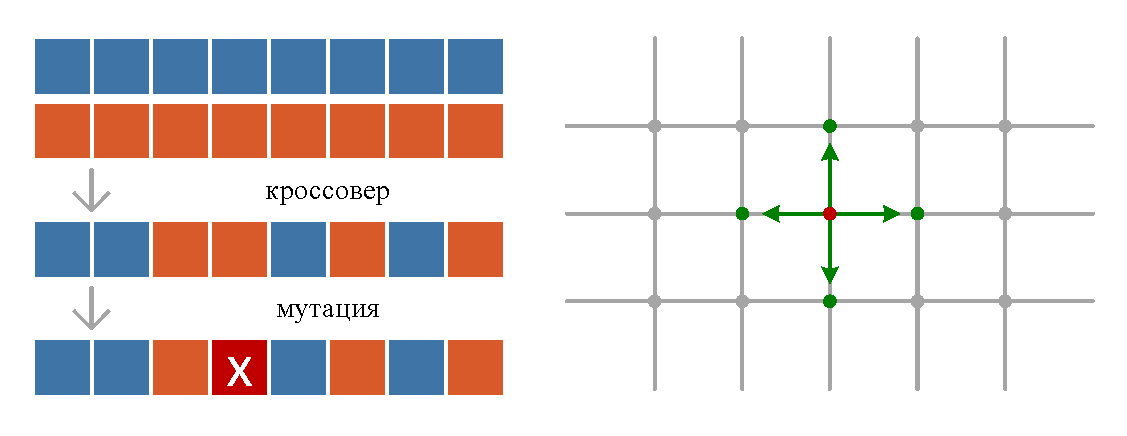
\includegraphics[width=0.7\textwidth]{fig/par_gen_cross-mut.pdf}
\singlespacing
\captionstyle{center}\caption{Схема кроссовера и мутации новой особи.}
\label{fig:text_2_genetic_cross_mut}
\end{figure}

Так как ген представляет собой номер опорной вершины дуального графа, то в качестве мутации выбрана операция замены случайной опорной вершины на выбранную случайным образом смежную с ней вершину (см. рис.~\ref{fig:text_2_genetic_cross_mut}, справа).

Рассмотренный генетический алгоритм поиска эффективной декомпозиции характеризуется следующими глобальными параметрами.
Количество эпох (\texttt{epochs\_count}) -- количество последовательных применяемых глобальных операций по вымиранию части популяции и ее восстановлению.
Размер популяции особей (\texttt{population\_size}) -- количество особей в популяции.
Доля вымирания (\texttt{extinction\_ratio}) – доля наименее эффективных особей, вымирающих на каждой эпохе.
Вероятность мутации (\texttt{mutation\_propability}) -- вероятность мутации в новой особи.

%Алгоритм применялся для решения задачи декомпозиции двумерной прямоугольной расчетной сетки размером $100 \times 100$ ячеек.
%Такой вид сетки выбран для удобства визуализации результатов, сам алгоритм применим для расчетных сеток произвольного вида, так как на вход он принимает только информацию о структуре дуального графа.

%Количество параметра \texttt{epochs\_count} выбрано равным 500.
%Алгоритм прекращает работу либо после обработки последней эпохи, либо после того, как все особи в популяции сравняются по характеристике эффективности.
%Размер популяции \texttt{population\_size} выбран равным 50.
%При выборе размера популяции необходимо придерживаться баланса.
%При слишком большом значении этого параметра время работы алгоритма существенно возрастает, а при слишком маленьком значении ограничивается разнообразие особей в популяции, что приводит к ранней остановке алгоритма в локальном минимуме, в котором все особи обладают одинаковым достаточно плохим показателем эффективности.
%Доля вымирания \texttt{extinction\_ratio} принята равной 0,2.
%При выборе доли вымирания не стоит использовать слишком высокие значения, так как это приводит к излишне интенсивному отсеву особей.
%Это может привести к преждевременной отбраковке средних по эффективности особей, способных дать более эффективное потомство.
%Вероятность возникновения мутации \texttt{mutation\_probability} принята равной 0,2.
%Ввиду того, что мутация представляет собой смещение опорной вершины по ребру к одному из своих соседей (что является достаточно незначительным изменением), то такое частое возникновение мутаций оправдано.

%\begin{figure}[ht]
%\centering
%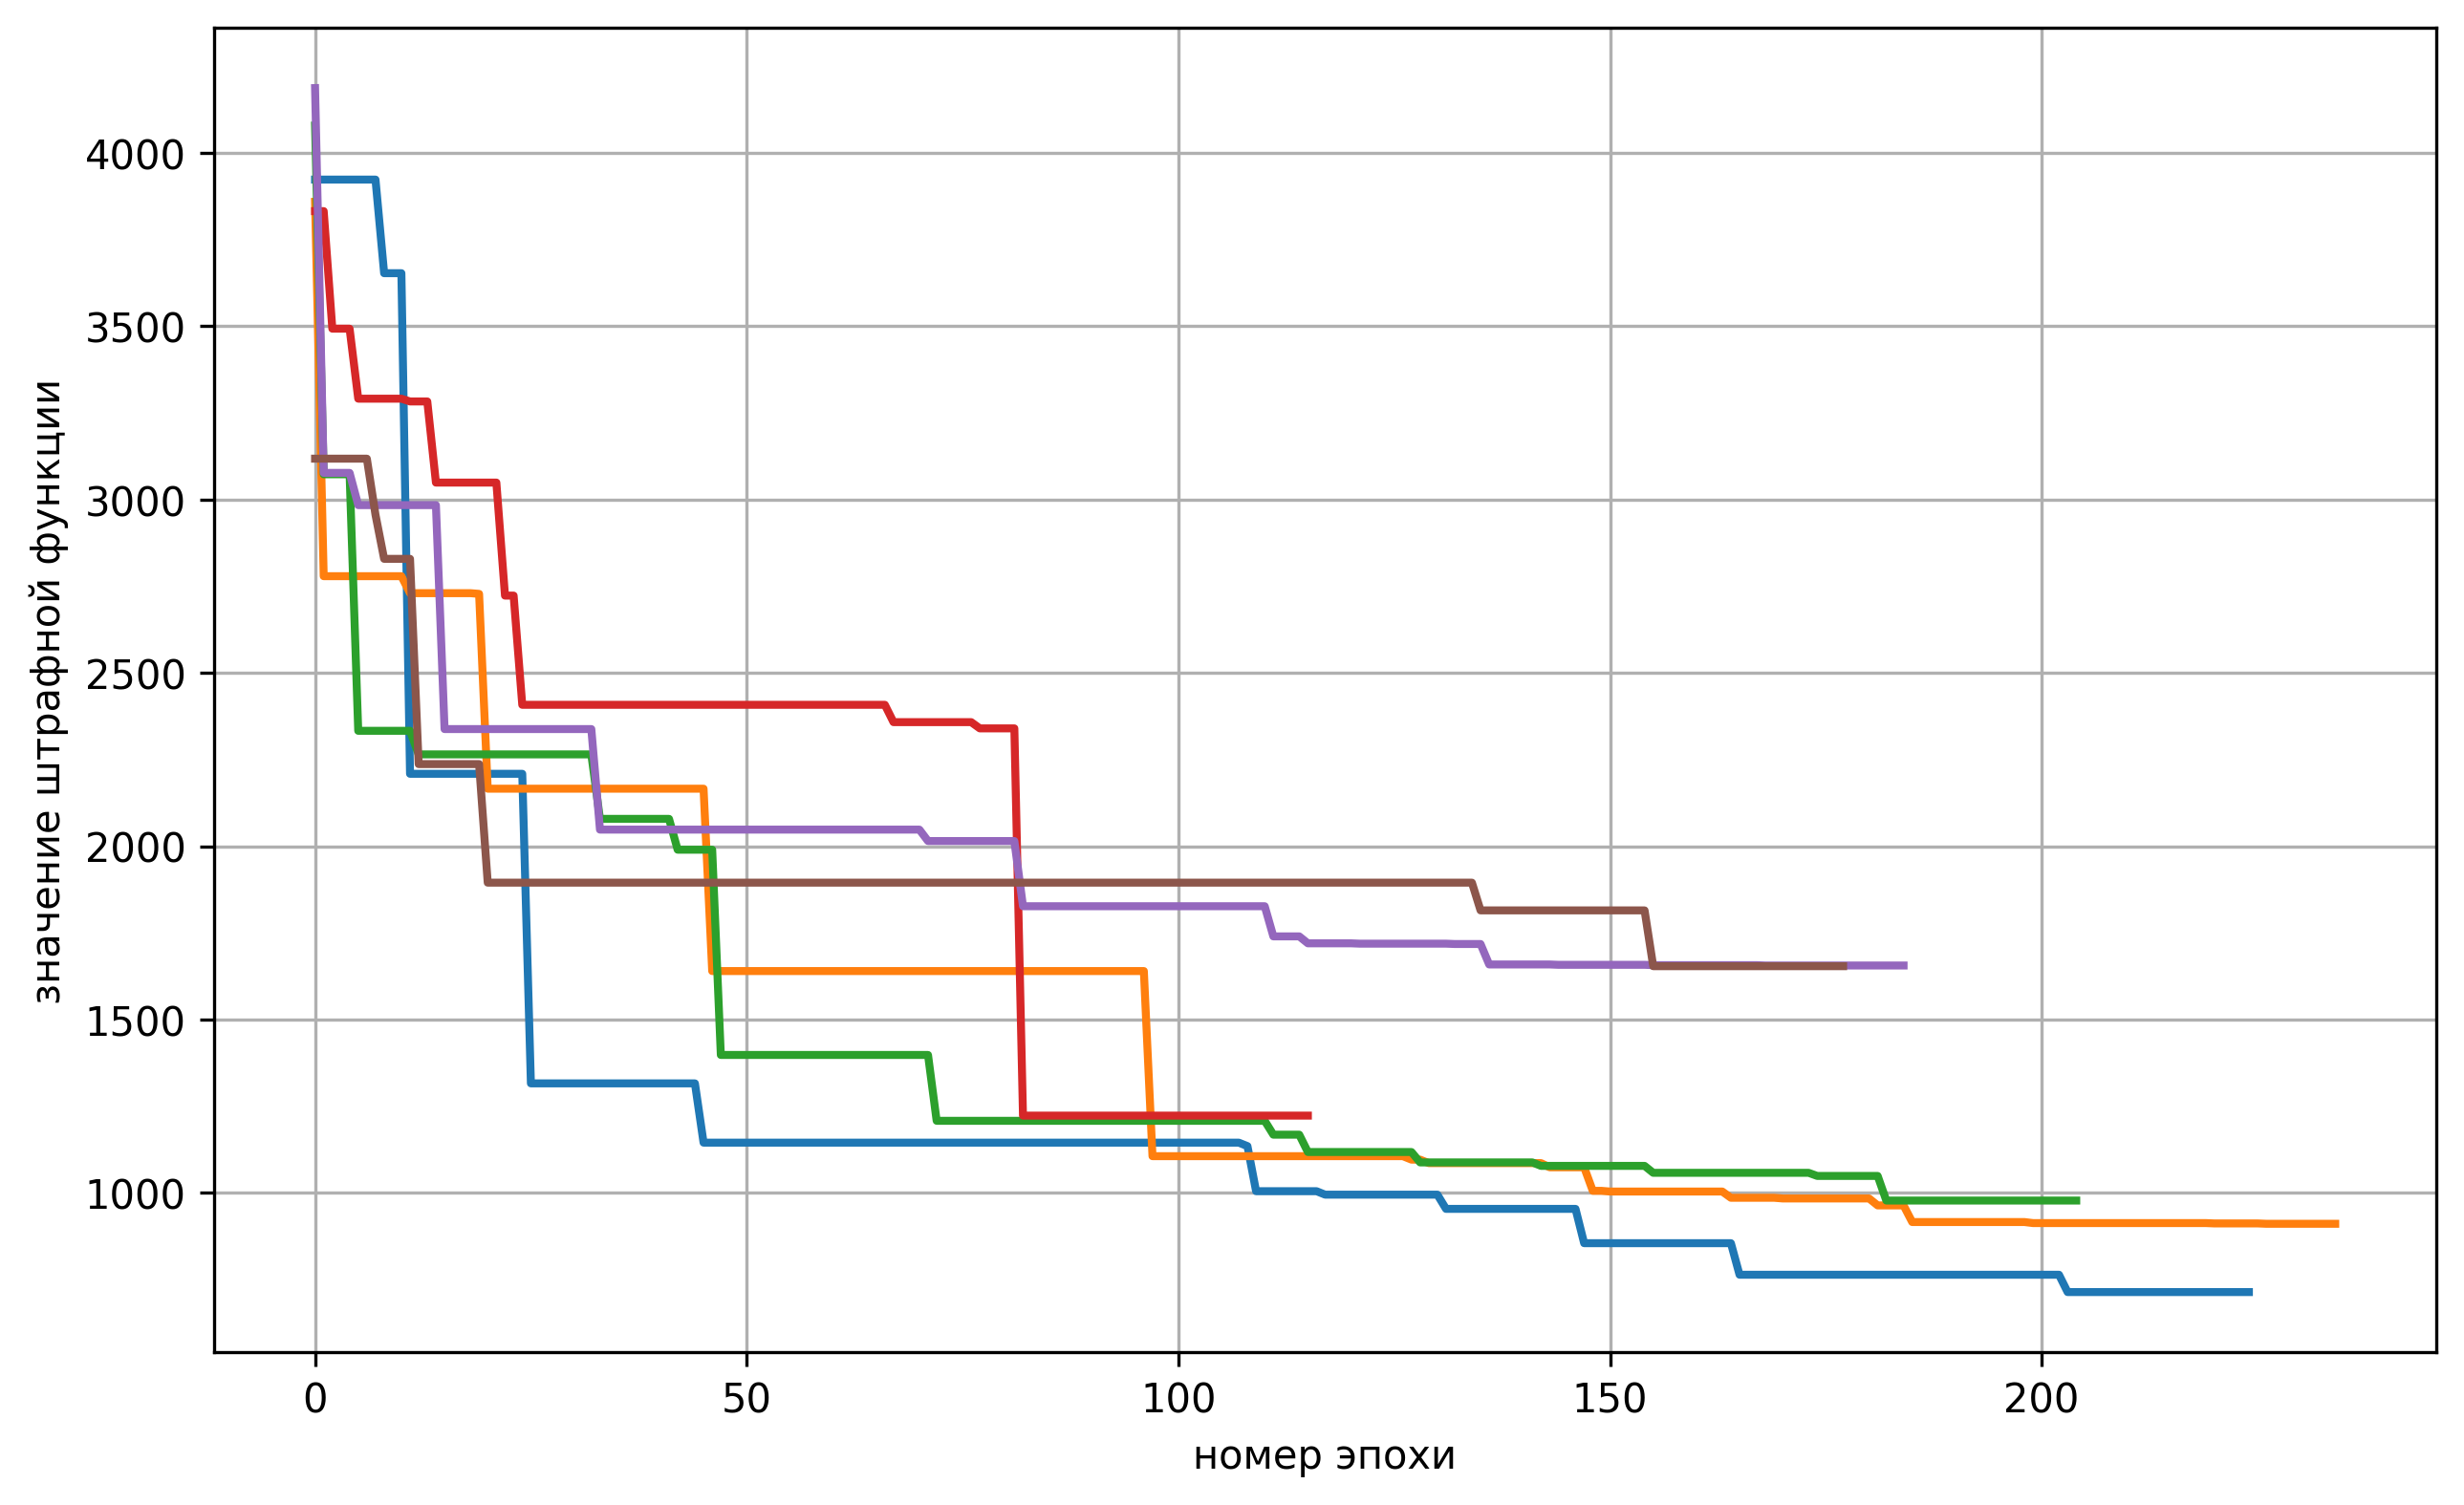
\includegraphics[width=0.8\textwidth]{fig/par_gen_chart1.png}
%\singlespacing
%\captionstyle{center}\caption{Характерные графики штрафной функции лучшей особи в популяции в зависимости от номера эпохи.}
%\label{fig:text_2_genetic_chart1}
%\end{figure}

%Типичные графики значения штрафной функции лучшей особи в популяции от номера эпохи приведены на рис.~\ref{fig:text_2_genetic_chart1}.
%Эксперименты показали, что при выбранном наборе макропараметров алгоритма примерно в первые 100 эпох наблюдается существенное улучшение лучшей особи в популяции, затем медленное %улучшение наблюдается еще около 150 эпох, после чего работа алгоритма останавливается в локальном минимуме при заполнении всей популяции копиями лучшей особи.
%При этом значение штрафной функции лучшей особи за время работы алгоритма падает примерно на 50-75\%, если считать от значения лучшей особи стартовой популяции.
%Для повышения качества работы алгоритма можно включить механизм предотвращения его ранней остановки.
%Для этого при возникновении копий лучшей особи можно применять к ней так называемые макромутации, что соответствует принудительному выталкиванию особи из локального минимума штрафной %функции \cite{Baranov2025Gen}.

\begin{figure}[ht]
\centering
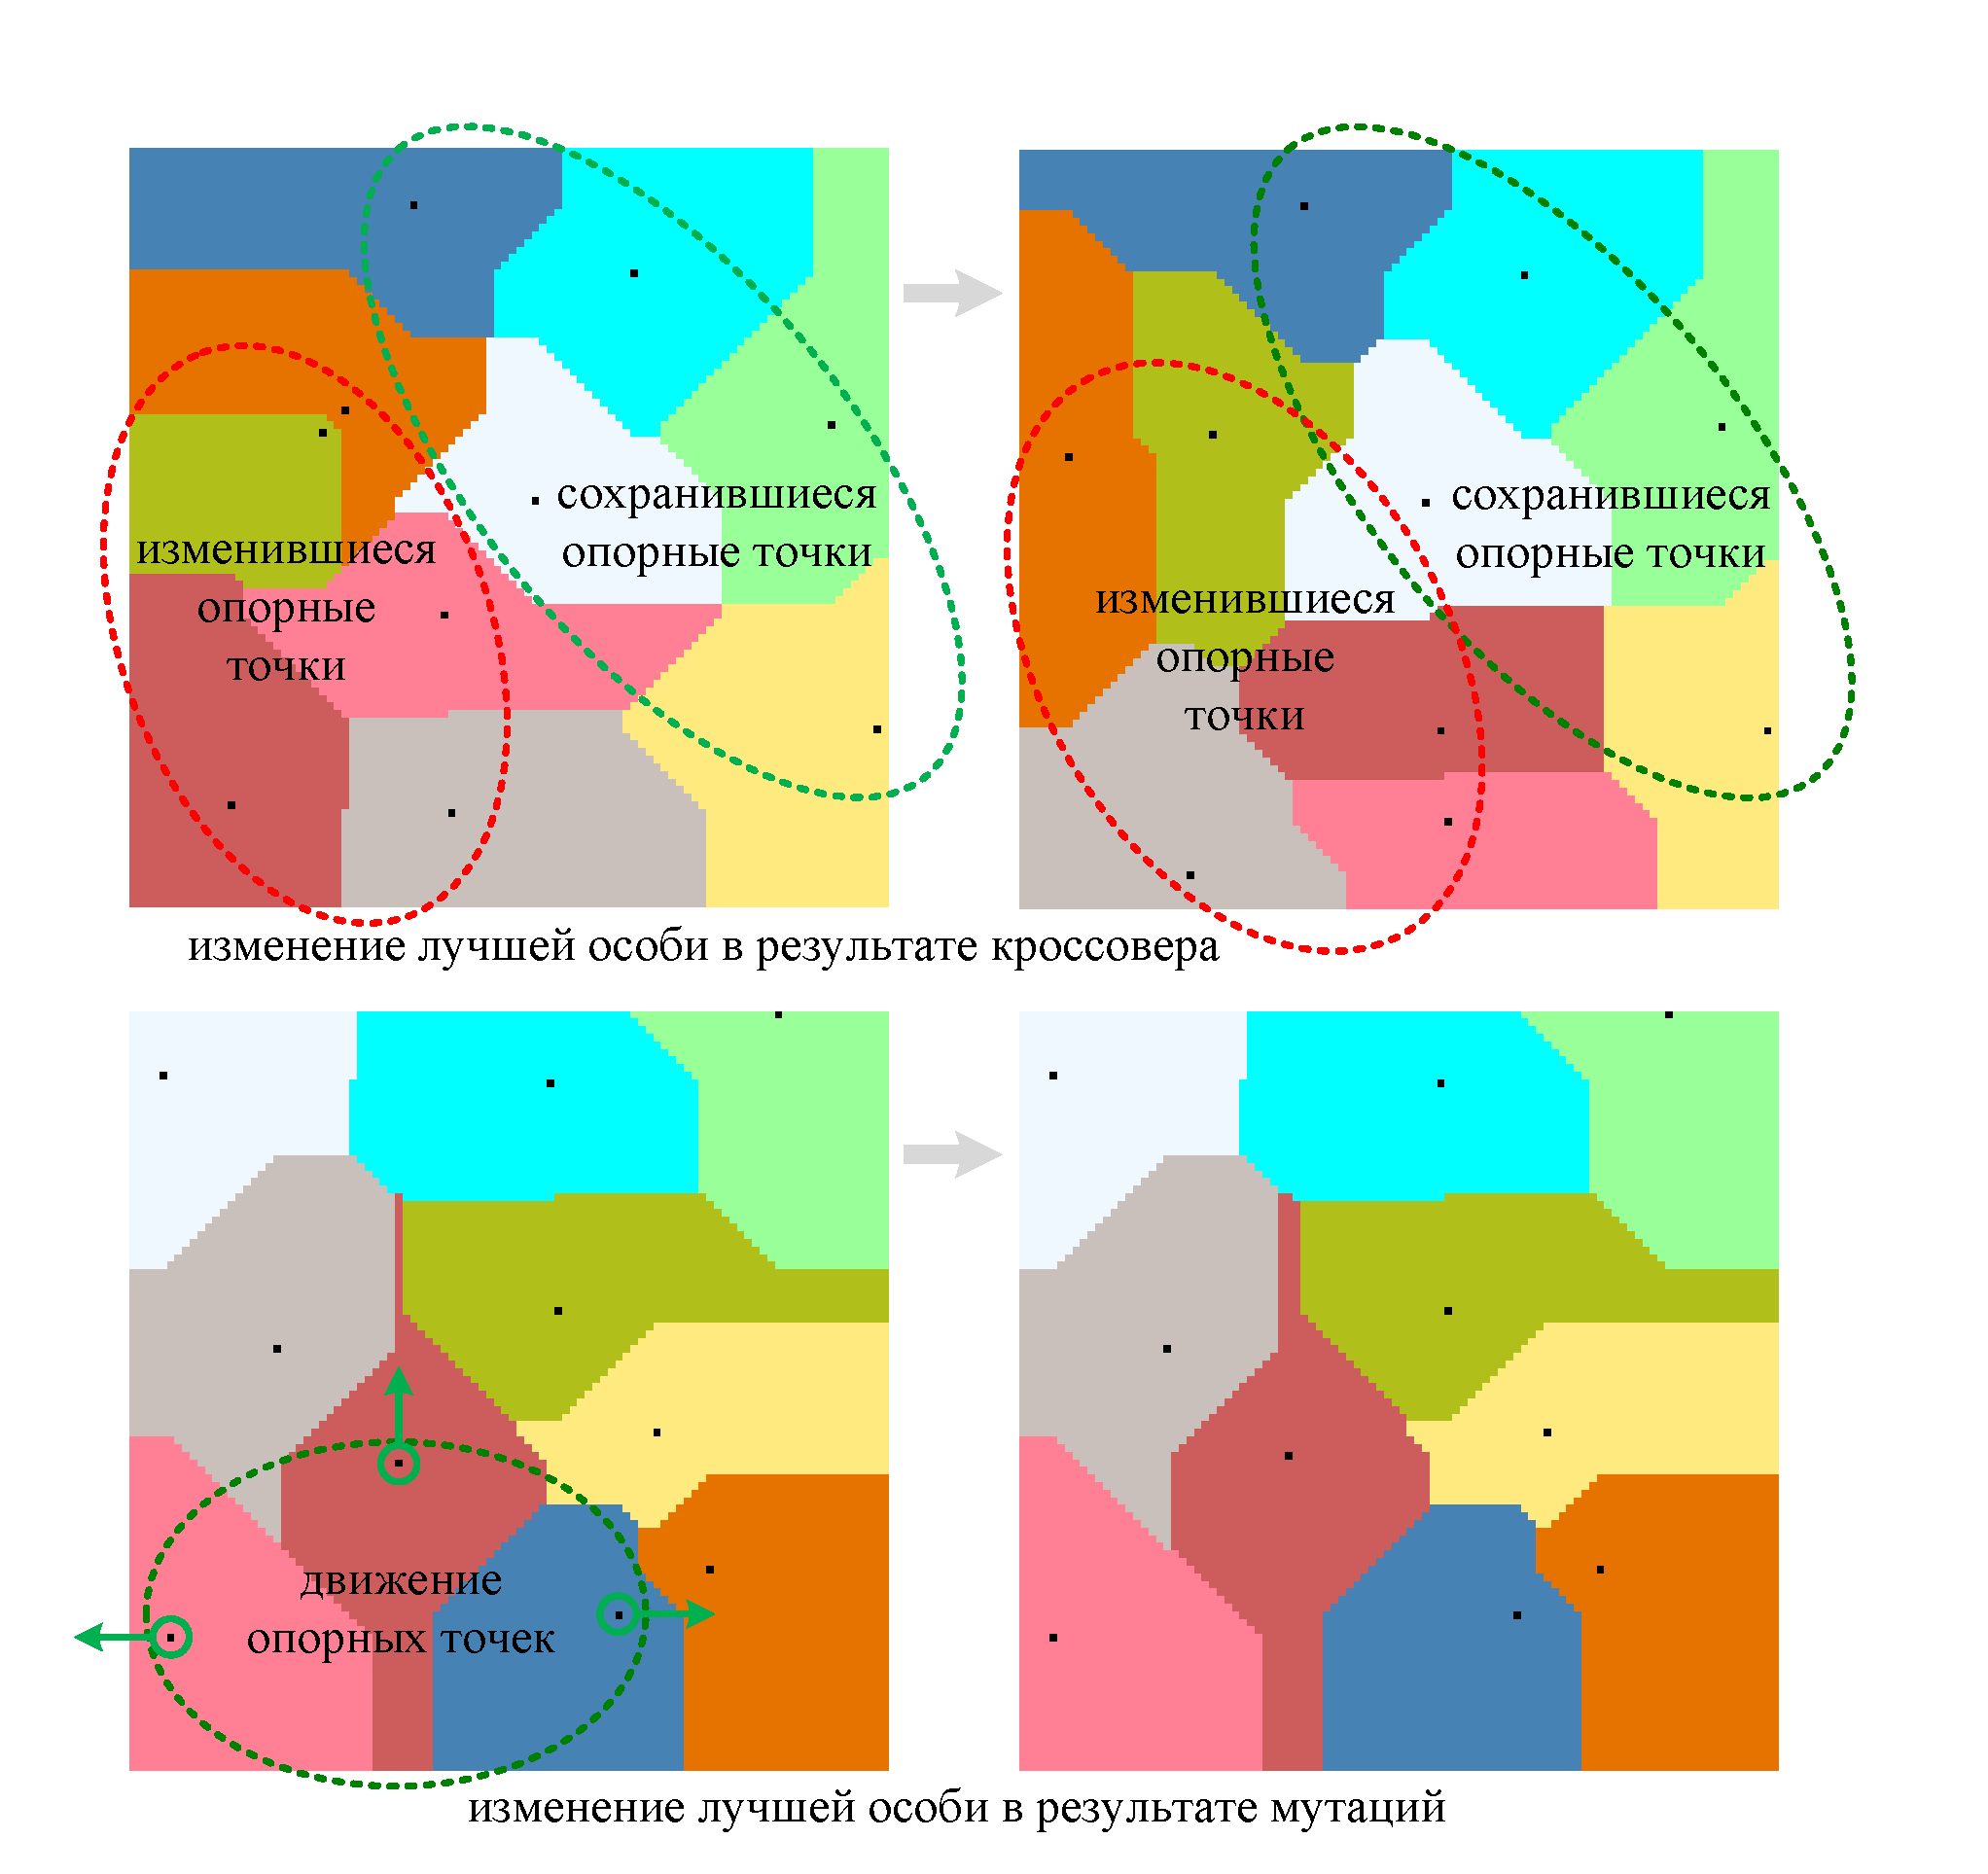
\includegraphics[width=0.8\textwidth]{fig/par_gen_changes.pdf}
\singlespacing
\captionstyle{center}\caption{Замещение части генотипа в процессе скрещивания (сверху), и мутация опорных вершин (снизу).}
\label{fig:text_2_genetic_changes}
\end{figure}

На рис.~\ref{fig:text_2_genetic_changes} приведены характерные варианты изменения лучшей особи при переходе от текущей популяции к популяции следующей эпохи.
Сверху на рисунке проиллюстрирована ситуация, когда часть опорных вершин лучшей особи сохранилась, а другая часть была заменена на опорные вершины второго родителя, что в целом привело к снижению значения штрафной функции.
Снизу на рисунке проиллюстрировано влияние последовательности мутаций на лучшую особь.
Так, даже незаметное на рисунке смещение опорных вершин привело к визуально различимому изменению геометрии образованных этими опорными вершинами доменов.

%\begin{figure}[ht]
%\centering
%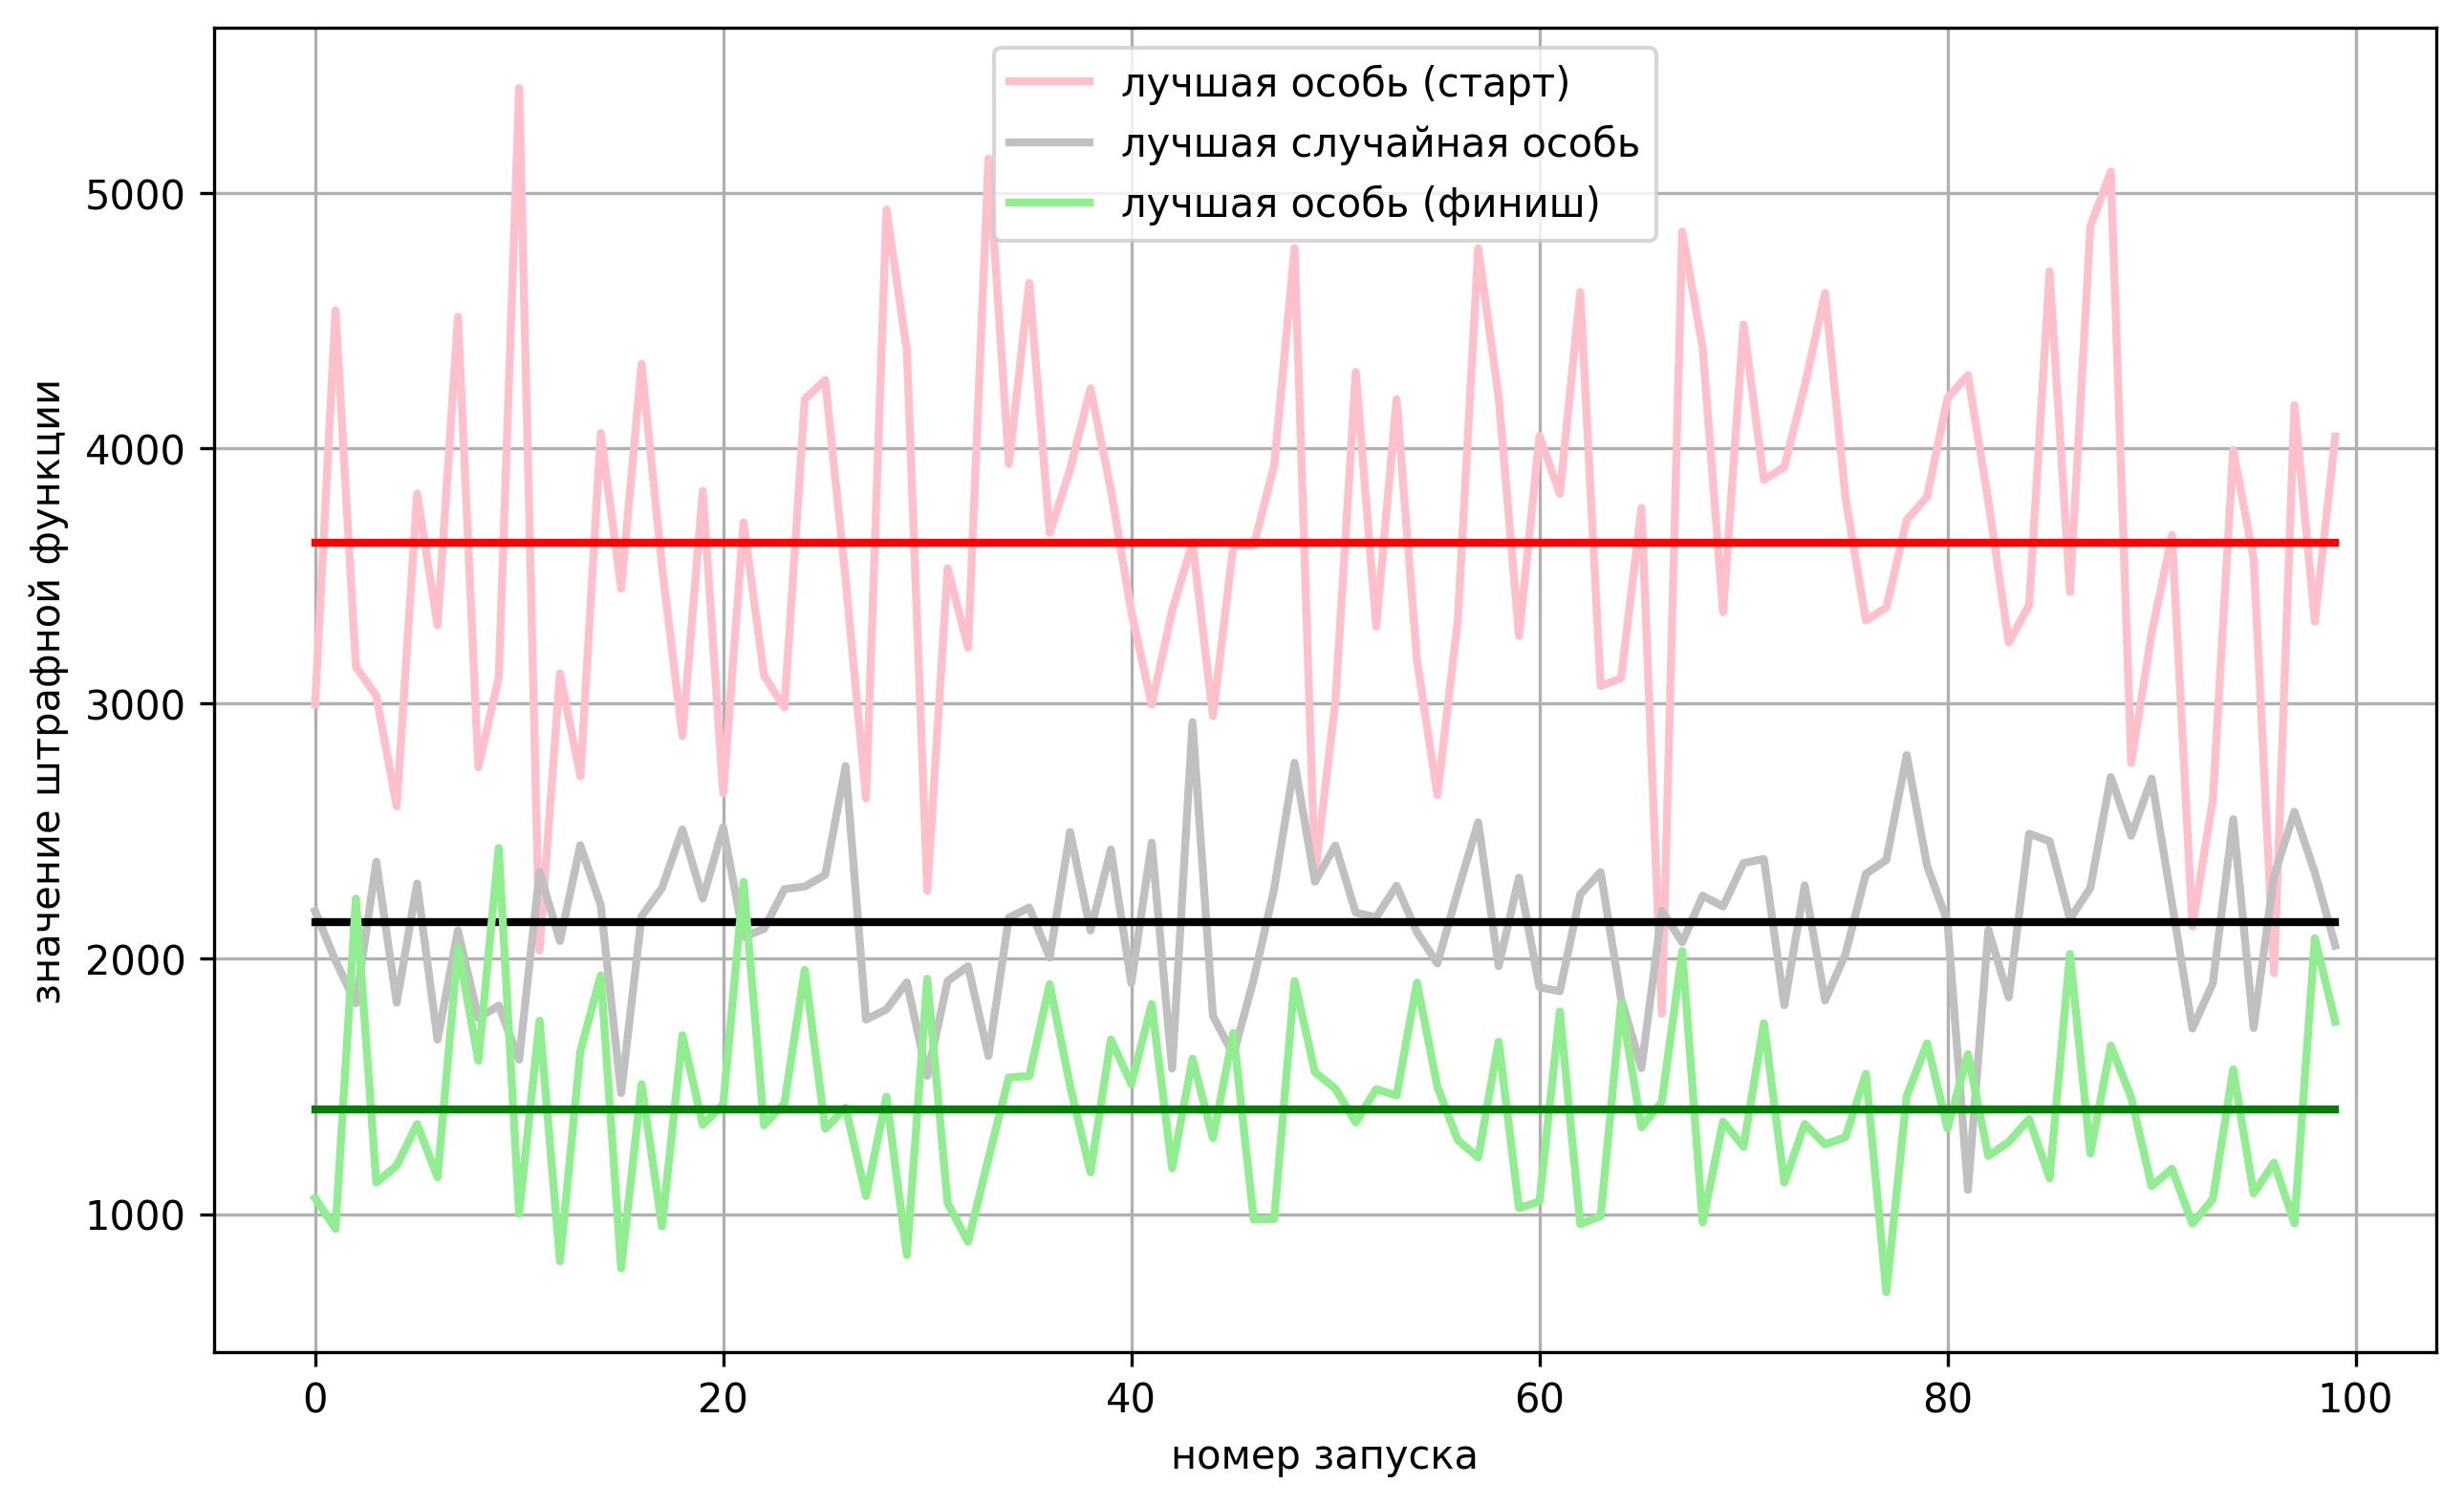
\includegraphics[width=0.8\textwidth]{fig/par_gen_chart2.png}
%\singlespacing
%\captionstyle{center}\caption{Сравнение лучшей особи в популяции генетического алгоритма с лучшей особью случайной популяции.}
%\label{fig:text_2_genetic_chart2}
%\end{figure}

%Следует отметить, что хоть реализация генетического алгоритма и подразумевает постоянное улучшение эволюционирующей популяции, это никак не гарантируется.
%Более того, при скрещивании двух особей нет гарантии, что их потомство будет более приспособленным к поставленной задаче.
%Также отсутствует гарантия, что применяемые мутации всегда приводят к более качественному решению.
%Поэтому возникает вопрос -- не является ли сам факт появления удачных особей случайным событием, и не было бы более эффективным просто сгенерировать большое количество случайных %особей, после чего выбрать из них лучшего представителя.
%Для проверки этого предположения были проведены следующие эксперименты.
%Пусть у нас имеется одиночный запуск генетического алгоритма с макропараметрами \texttt{population\_size} и \texttt{extinction\_ratio}.
%Если в процессе работы алгоритма до его завершения прошло \texttt{ecount} эпох (не считая стартовой), то всего было создано \texttt{icount} = \texttt{population\_size} × (1 + %\texttt{ecount} × \texttt{extinction\_ratio}) особей.
%Поэтому после завершения каждого запуска генетического алгоритма его результат сравнивался со значением лучшей особи из случайной популяции размера \texttt{icount}.
%Результаты такого сравнения приведены на рис.~\ref{fig:text_2_genetic_chart2}.
%Красным цветом отмечен график качества лучшей особи в начале работы алгоритма, зеленым -- в конце.
%Черным цветом отмечено значение лучшей особи случайной популяции размера \texttt{icount}.
%Также на графиках отмечены линии средних значений для серии запусков генетического алгоритма.
%Результаты расчетов показали, что лучшая особь популяции генетического алгоритма опережает лучшую особь случайной популяции примерно в 1,5 раза.

Генетический алгоритм применим к расчетным сеткам произвольного вида, с его помощью можно быстро получать качественное решение декомпозиции, произвольным образом задавая требуемую штрафную функции решения.
Алгоритм допускает параллельное исполнение, хорошо масштабируется для работы с расчетными сетками большего размера.
Генетический алгоритм требует для своего применения эффективной реализации процедуры обхода графа в ширину от инициирующих вершин.

% Сглаживание границ доменов.
\subsubsection{Сглаживание границ между доменами поверхностной \mbox{расчетной} сетки}\label{sec:text_2_smooth}

При использовании декомпозиции расчетной сетки основным показателем качества декомпозиции является параметр $D$, так как он отражает равномерность распределения ячеек по доменам.
Однако если игнорировать остальные показатели, то в процессе декомпозиции могут появляться протяженные <<пилообразные>> границы между доменами, которые приводят к возрастанию показателей $L$ и $I$, что негативно сказывается на производительности.
Пример возникновения таких пилообразных границ можно увидеть на рис.~\ref{fig:text_2_decompsurf_4} снизу справа, на рис.~\ref{fig:text_2_smooth_bad_border} фрагмент сетки с пилообразными границами между доменами приведен более крупно.

\begin{figure}[ht]
\centering
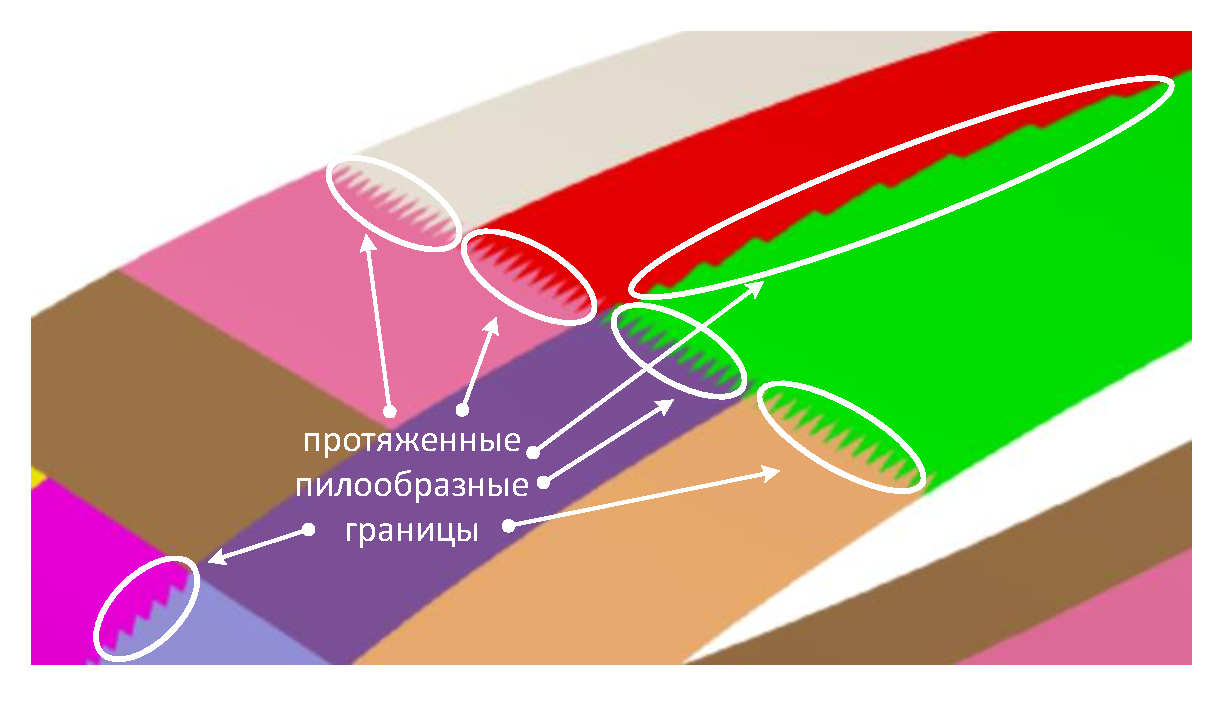
\includegraphics[width=0.6\textwidth]{fig/par_bad-border.pdf}
\singlespacing
\captionstyle{center}\caption{Возникновение протяженных пилообразных границ между доменами.}
\label{fig:text_2_smooth_bad_border}
\end{figure}

Такие границы необходимо отдельно обрабатывать с целью сокращения их длины.
При использовании алгоритмов декомпозиции, основанных на наращивании доменов путем обхода графа в ширину, образуются более сглаженные границы, однако из-за этого деградирует параметр качества декомпозиции $D$.
Возникновение протяженных пилообразных границ между доменами особенно характерно для неструктурированных поверхностных сеток, на которых зачастую встречаются ячейки с очень острыми углами.
Будем рассматривать алгоритм сглаживания границ между доменами, на который накладывается требование сохранения значения показателя $D$ \cite{Bagrov2021Smooth}.

Алгоритм сглаживания границ между доменами носит локальный характер, он применяется последовательно к каждой паре доменов и направлен на уменьшение длины границы между ними с сохранением баланса количества ячеек в этих доменах.
Граница между двумя доменами может быть представлена в виде набора простых циклов и простых цепей.
При этом простой цикл может быть обработан таким же образом, как и простая цепь, с учетом совпадения первого и последнего узла этой цепи (для такого виртуального размыкания простого цикла может быть выбран произвольный узел этого цикла).
В процессе применения алгоритма сглаживания может быть выполнено виртуальное размыкание всех простых циклов, после чего все образовавшиеся цепи рассматриваются последовательно.
Без ограничения общности можно считать, что мы работаем с одной простой цепью (полученной с помощью записи всех отдельных простых цепей подряд), представляющей границу между парами доменов.

Вначале одним проходом по цепи выполняется поиск всех пригодных для сглаживания границы шаблонов, представленных на рис.~\ref{fig:text_2_smooth_smooth_border}.

\begin{figure}[ht]
\centering
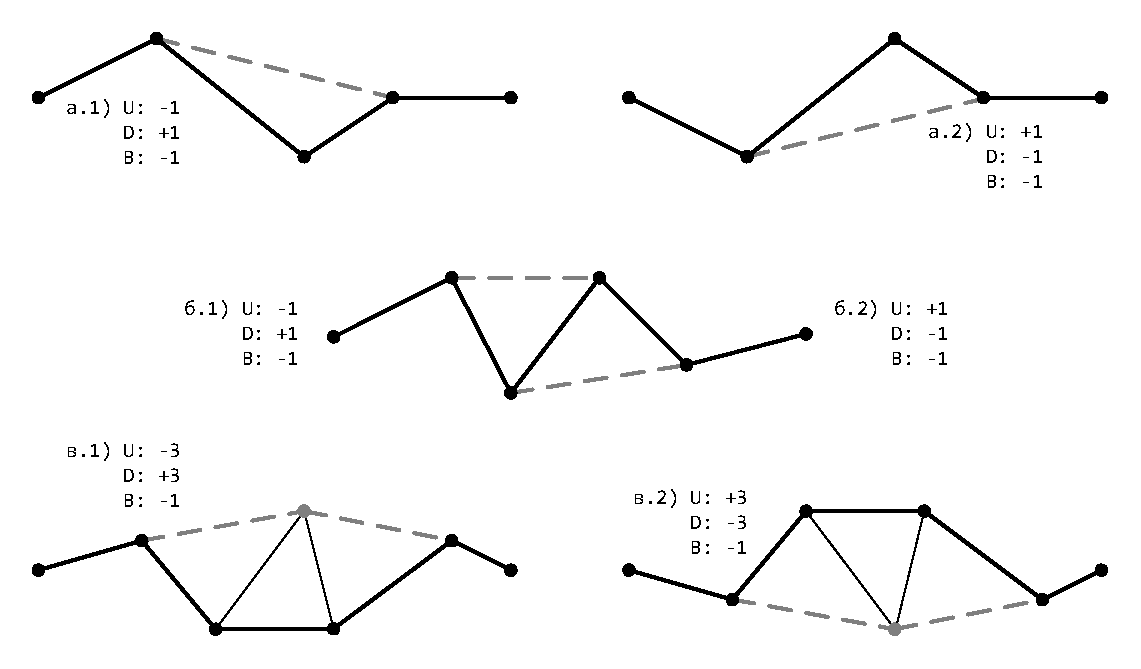
\includegraphics[width=0.8\textwidth]{fig/par_smooth-border.pdf}
\singlespacing
\captionstyle{center}\caption{Шаблоны элементарных действий сглаживания границ между доменами.}
\label{fig:text_2_smooth_smooth_border}
\end{figure}

На рис.~\ref{fig:text_2_smooth_smooth_border} представлены 5 шаблонов, которые мы будем использовать для уменьшения длины границы между двумя доменами.
Рассмотрим шаблон а.1.
На нем обозначена часть границы между двумя доменами (домен сверху от ломаной обозначен буквой $U$, домен снизу от ломаной обозначен буквой $D$.
Черной сплошной линией прочерчена текущая граница между доменами.
Пунктирной линией показано возможное улучшение, которое в рассматриваемом случае приведет к следующим последствиям: уменьшение количества ячеек верхнего домена на 1 ($U: -1$), увеличение количества ячеек нижнего домена на 1 ($D: + 1$), уменьшение длины границы между двумя доменами на 1 ($B: -1$).
Таким образом, шаблон а.1 направлен на втягивание одной ячейки из верхнего домена в нижний домен с сокращением длины границы на единицу.
Шаблон а.2 выполняет симметричное действие по втягиванию одной ячейки из нижнего домена в верхний домен, также сокращая при этом длину границы на единицу.
Шаблоны в.1 и в.2 выполняют аналогичные действия, однако вместо одной ячейки происходит втягивание сразу трех соседних ячеек с одновременным уменьшением длины границы между доменами на единицу. Отдельно стоит отметить шаблоны б.1 и б.2.
Они представляют собой один шаблон в рамках которого может быть осуществлено втягивание либо ячейки из нижнего домена в верхний, либо наоборот, но не одновременно (в противном случае длина границы останется неизменной).
Можно рассматривать и более сложные шаблоны, однако существенного прироста производительности они уже не дают, но приводят к усложнению алгоритма.

После того, как внутри цепи найдены все шаблоны, потенциально пригодные для оптимизации границы, выполняется разметка того, как найденные шаблоны могут влиять друг на друга.
С учетом того, что любой шаблон может повлиять только на своих непосредственных соседей, такое действие также выполняется с линейной сложностью относительно длины границы.

Центральным местом работы алгоритма является выбор такого множества шаблонов, которые не влияют друг на друга (то есть могут быть применены все одновременно) и не нарушают суммарного баланса ячеек (так как для нас важнейшим показателем эффективности декомпозиции расчетной сетки является равномерность распределения ячеек по доменам).
После выбора наибольшего возможного набора шаблонов они применяются, и на этом обработка цепи считается завершенной.

Рассмотрим более подробно алгоритм выбора максимального подмножества неконфликтующих шаблонов, не нарушающих общий баланс ячеек между парой доменов.
Для этого рассмотрим пример, представленный на рис.~\ref{fig:text_2_smooth_smooth}

\begin{figure}[ht]
\centering
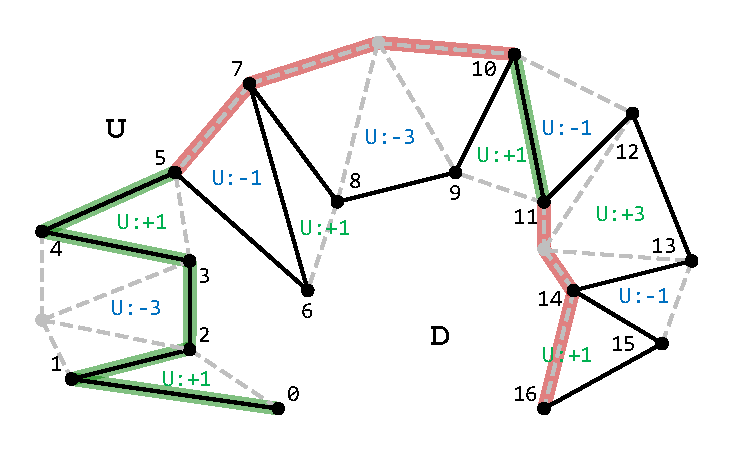
\includegraphics[width=0.8\textwidth]{fig/par_smooth.pdf}
\singlespacing
\captionstyle{center}\caption{Алгоритм сглаживания границы между доменами.}
\label{fig:text_2_smooth_smooth}
\end{figure}

На рис.~\ref{fig:text_2_smooth_smooth} представлена граница между двумя доменами (они условно обозначены $U$ -- верхний и $D$ -- нижний) в виде простой цепи $0-16$.
Шаблон, который может быть применен для сглаживания границы будем обозначать $t_{a-b}$, где $a$ -- номер стартовой вершины, а $b$ -- номер конечной вершины ($b > a$).
На рис.~\ref{fig:text_2_smooth_smooth} можно выделить следующее множество шаблонов
\begin{equation}
T = \{ t_{0-2}, t_{1-4}, t_{3-5}, t_{5-7}, t_{6-8}, t_{7-10}, t_{9-11}, t_{10-12}, t_{11-14}, t_{13-15}, t_{14-16} \}.
\end{equation}

Использование каждого из приведенных шаблонов уменьшает длину границы, но нарушает баланс ячеек между доменами.
Будем использовать функцию $U(t)$, которая обозначает изменение баланса ячеек по отношению к домену $U$ из-за применения шаблона $t$.
Так $U(t_{7-10}) = -3$, что означает, что при применении шаблона $t_{7-10}$ домен $U$ потеряет 3 ячейки.

\begin{definition}
Пусть даны два шаблона $t_{a-b}$ и $t_{c-d}$.
Будем говорить, что $t_{a-b} = t_{c-d}$, если $a = c$, $b = d$.
Также будем говорить, что $t_{a-b} < t_{c-d}$, если $a < c$.
\end{definition}

\begin{definition}
Два шаблона $t_{a-b} < t_{c-d}$ назовем конфликтующими (или пересекающимися по ребрам), если $c < b$, и будем обозначать $t_{a-b} \cap t_{c-d} \ne \emptyset$.
\end{definition}

На рис.~\ref{fig:text_2_smooth_smooth} каждая пара соседних шаблонов кроме $\{ t_{3-5}$, $t_{5-7} \}$ является конфликтующей.
Два конфликтующих шаблона применить одновременно нельзя, так как это либо невозможно технически, либо не приведет к уменьшению длины границы.

\begin{figure}[!ht]
\centering
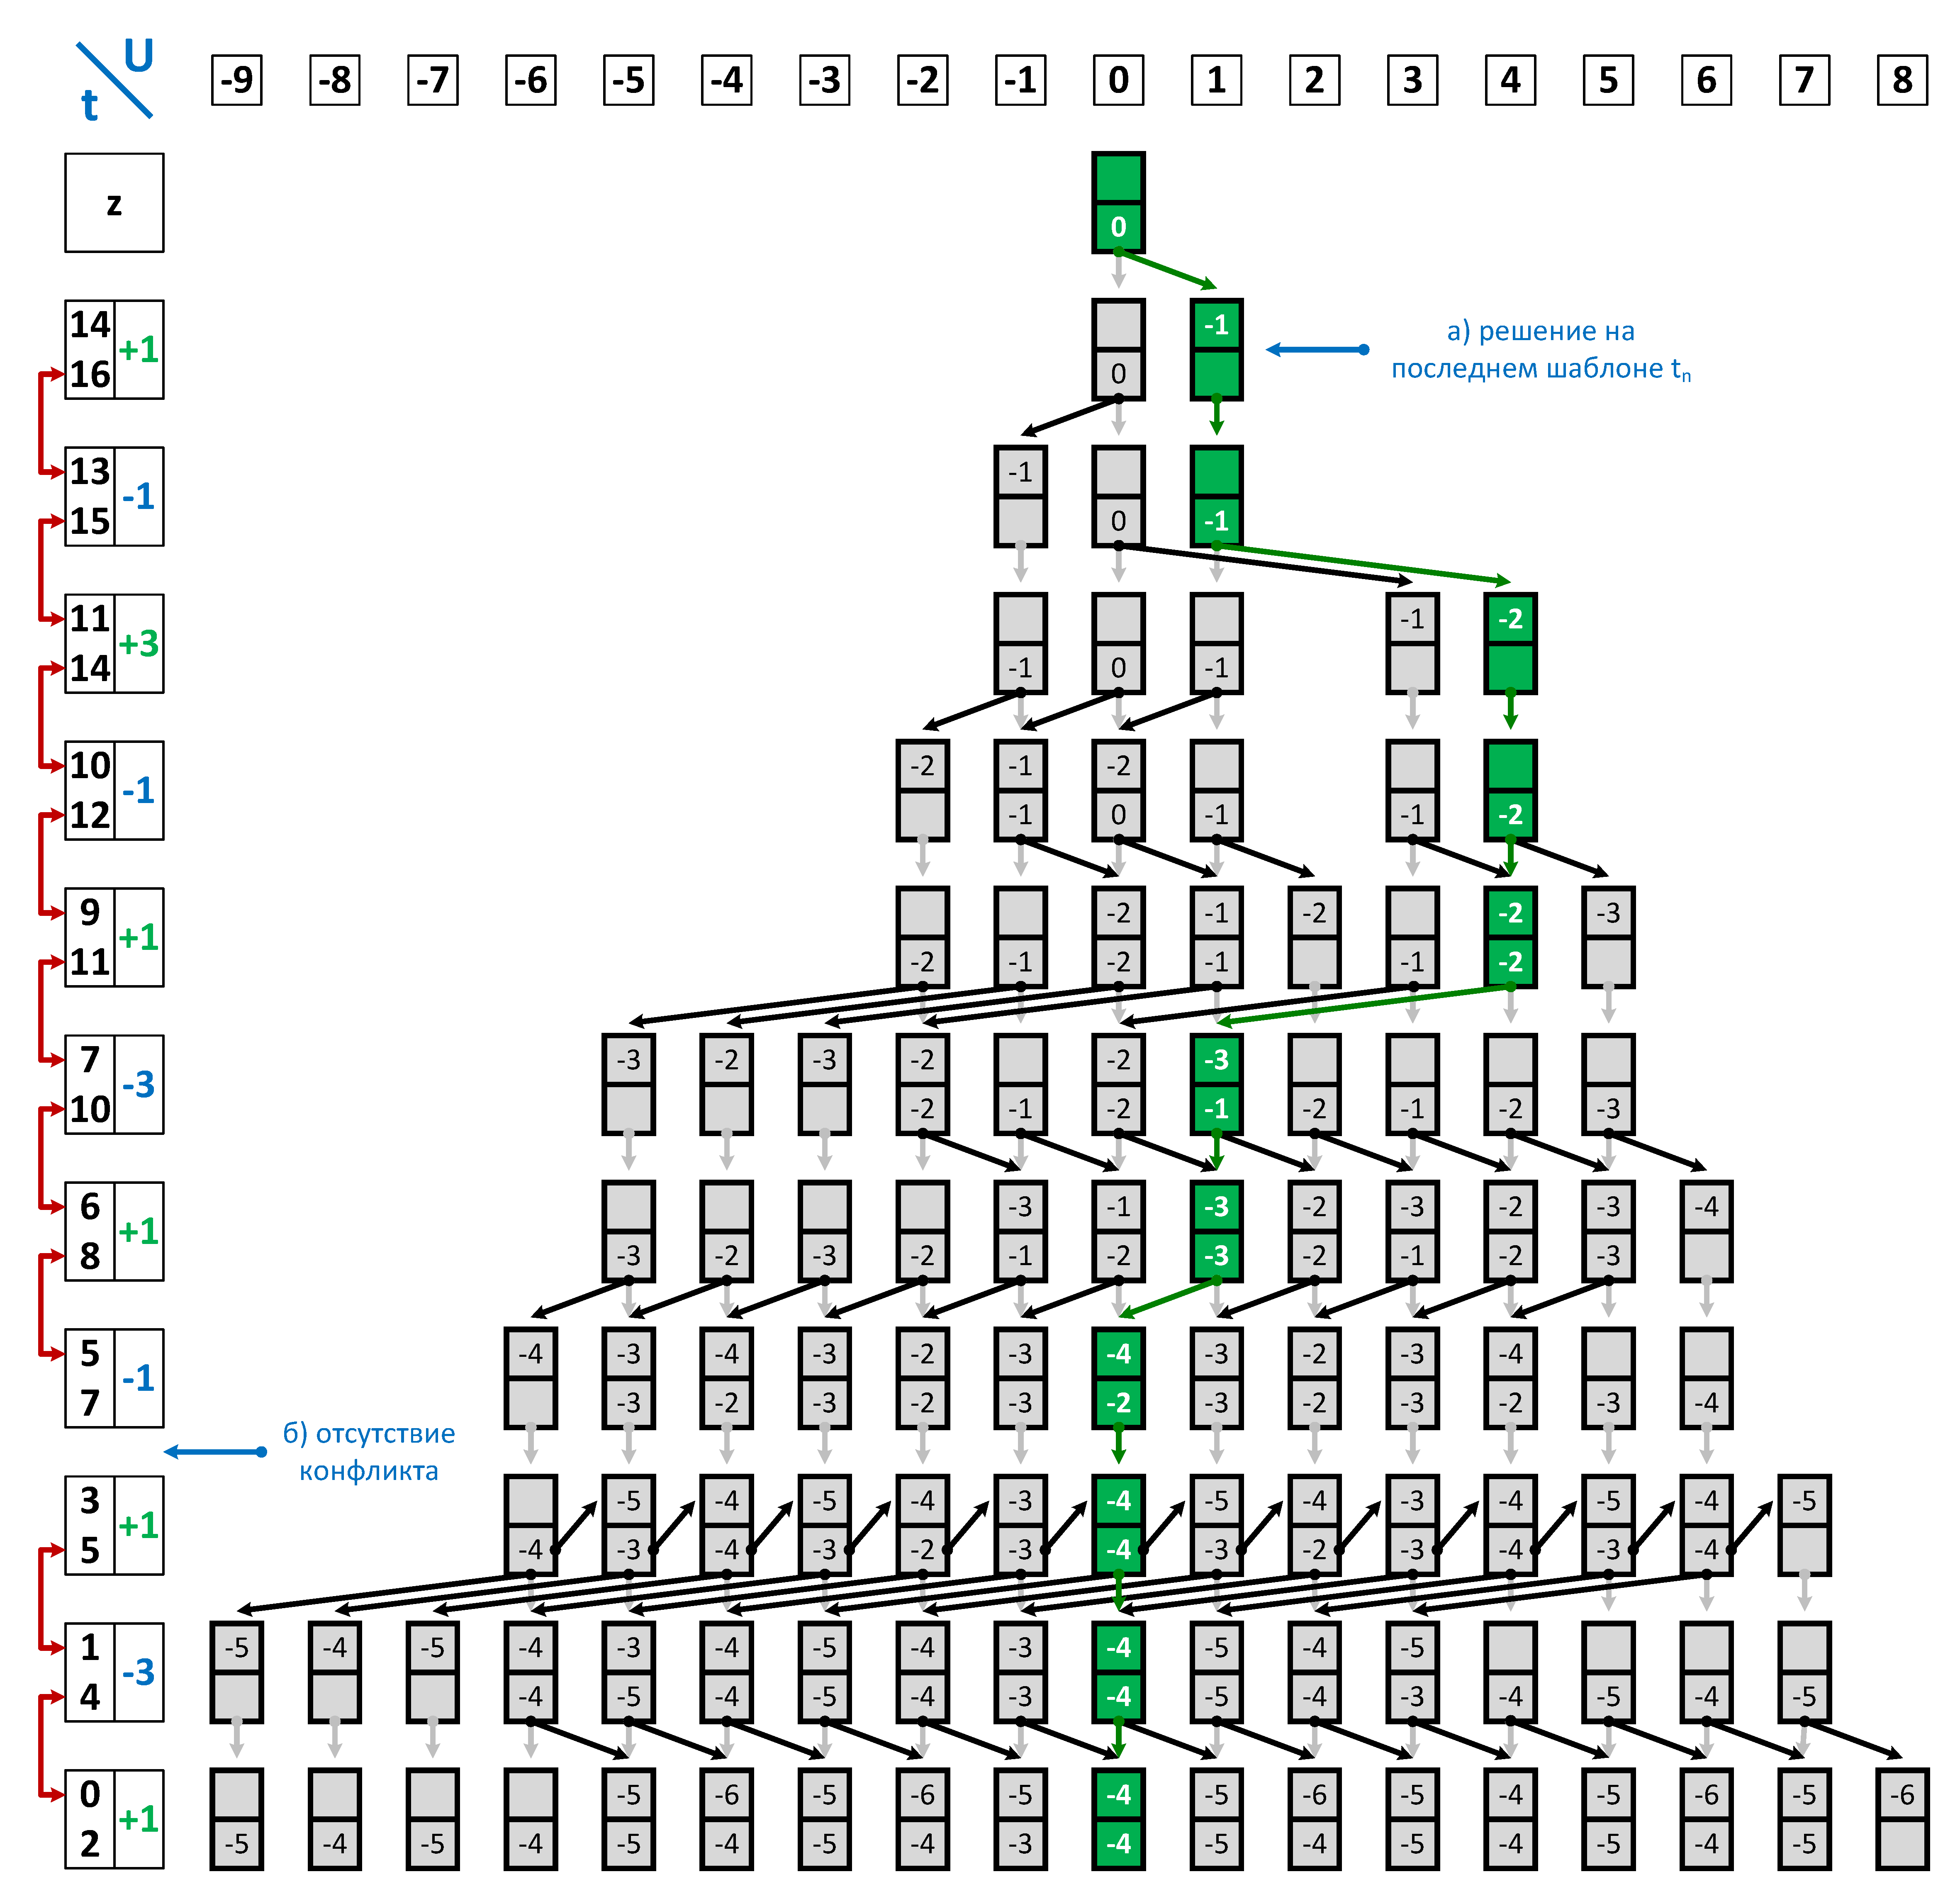
\includegraphics[width=1.0\textwidth]{fig/par_smooth-scheme-cut.pdf}
\singlespacing
\captionstyle{center}\caption{Схема поиска решения задачи сглаживания границы между доменами.}
\label{fig:text_2_smooth_smooth_scheme}
\end{figure}

Ввиду того, что применение каждого отдельного шаблона уменьшает длину границы на 1, задача поиска оптимального решения может быть сформулирована в виде поиска в множестве шаблонов подмножества максимального размера, не содержащего конфликтующих шаблонов.
Поставленную задачу будем решать методом динамического программирования (схема работы алгоритма для примера с рис.~\ref{fig:text_2_smooth_smooth} представлена на рис.~\ref{fig:text_2_smooth_smooth_scheme}).
Для этого рассмотрим функцию $B(t, u, x)$, отражающую изменение длины границы при решении задачи на множестве шаблонов $\{ t' \in T : t' \ge t \}$ при условии изменения количества ячеек в домене $U$ на $u$ единиц.
Параметр $x$ является булевым и принимает значение $1$, если шаблон $t$ вошел в решение, и $0$ -- в противном случае.
Решением поставленной задачи является значение $\min(B(t_0, 0, 1), B(t_0, 0, 0))$, где $t_0$ -- первый шаблон на рассматриваемой цепи, в нашем случае это $t_{0-2}$.

Решение задачи начинается с последнего шаблона $t_n$ (в нашем случае это $t_{14-16}$) (см. рис.~\ref{fig:text_2_smooth_smooth_scheme}, а).
Для него все множество используемых шаблонов состоит только из него самого, и
\begin{equation}
	\left\{
		\begin{aligned}
			& B(t_n, 0, 0) = 0 \\
			& B(t_n, U(t_n), 1) = -1
		\end{aligned}
	\right.
\end{equation}
для всех остальных значений $u$ значение функции $B(t_n, u, x)$ не определено, будем считать его равным $+\infty$ (это означает, что на последнем шаблоне кроме значений $0$ и $U(t_n)$ недостижимы другие значения изменения количества ячеек в домене $U$).

Пусть задача решена для некоторого шаблона $t_{k + 1}$.
Рассмотрим переход к решению для шаблона $t_k$.
Сначала все значения $B(t_k, u, x)$ принимаются равными $+\infty$.

Во-первых, имея любое допустимое решение для шаблона $t_{k + 1}$ мы можем получить решение для шаблона $t_k$, просто проигнорировав этот шаблон, то есть для всех $u$, для которых найдено решение для шаблона $t_{k + 1}$, выполним следующую операцию (на рис.~\ref{fig:text_2_smooth_smooth_scheme} представлена серыми стрелками):
\begin{equation}
	B(t_k, u, 0) = \min \left( B(t_{k + 1}, u, 0), B(t_{k + 1}, u, 1) \right).
\end{equation}

Игнорирование шаблона $t_k$ не меняет баланс ячеек между доменами, из рис.~\ref{fig:text_2_smooth_smooth_scheme} это видно, так как все серые стрелки направлены строго вниз.

Второй момент связан с попыткой использования шаблона $t_k$.
Если $t_k \cap t_{k + 1} = \emptyset$, то есть конфликта нет (см. рис.~\ref{fig:text_2_smooth_smooth_scheme}, б), то шаблон $t_k$ можно использовать вне зависимости от того, был ли использован шаблон $t_{k + 1}$.
То есть для всех $u$, для которых было найдено решение для шаблона $t_{k + 1}$ выполним следующее действие:
\begin{equation}
	B(t_k, u + U(t_k), 1) = B(t_k, u, 0) - 1.
\end{equation}

И наконец в случае конфликтующих $t_k$ и $t_{k + 1}$ мы можем использовать шаблон $t_k$ только в том случае, если не был использован шаблон $t_{k + 1}$, то есть для всех $u$ для которых $B(t_{k + 1}, u, 0) \ne +\infty$ нужно выполнить операцию
\begin{equation}
	B(t_k, u + U(t_k), 1) = B(t_{k + 1}, u, 0) - 1.
\end{equation}

В результате работы алгоритма получим все наилучшие варианты использования шаблонов для заданного изменения баланса ячеек между доменами $U$ и $D$, в частности для нулевого изменения баланса.
На рис.~\ref{fig:text_2_smooth_smooth_scheme} зеленым цветом выделен путь для достижения наилучшего сокращения пути при сохранении баланса ячеек между доменами.
В нашем случае одним (но не единственным) из оптимальных решений является использование шаблонов $t_{14-16}$, $t_{11-14}$, $t_{7-10}$, $t_{5-7}$, что сокращает границу между доменами на 4, это решение отражено на рис.~\ref{fig:text_2_smooth_smooth}.

В результате работы алгоритма рассчитываются оптимальные решения для всех значений $u$ из диапазона
\begin{equation}
	[U_{min}, U_{max}] = \left[ \frac{1}{2} \sum_{t \in T}{(U(t) - |U(t)|)}, \frac{1}{2} \sum_{t \in T}{(U(t) + |U(t)|)} \right],
\end{equation}
а сложность алгоритма равна $O \left( |T| \cdot (U_{max} - U_{min} + 1) \right)$.

\begin{figure}[ht]
\centering
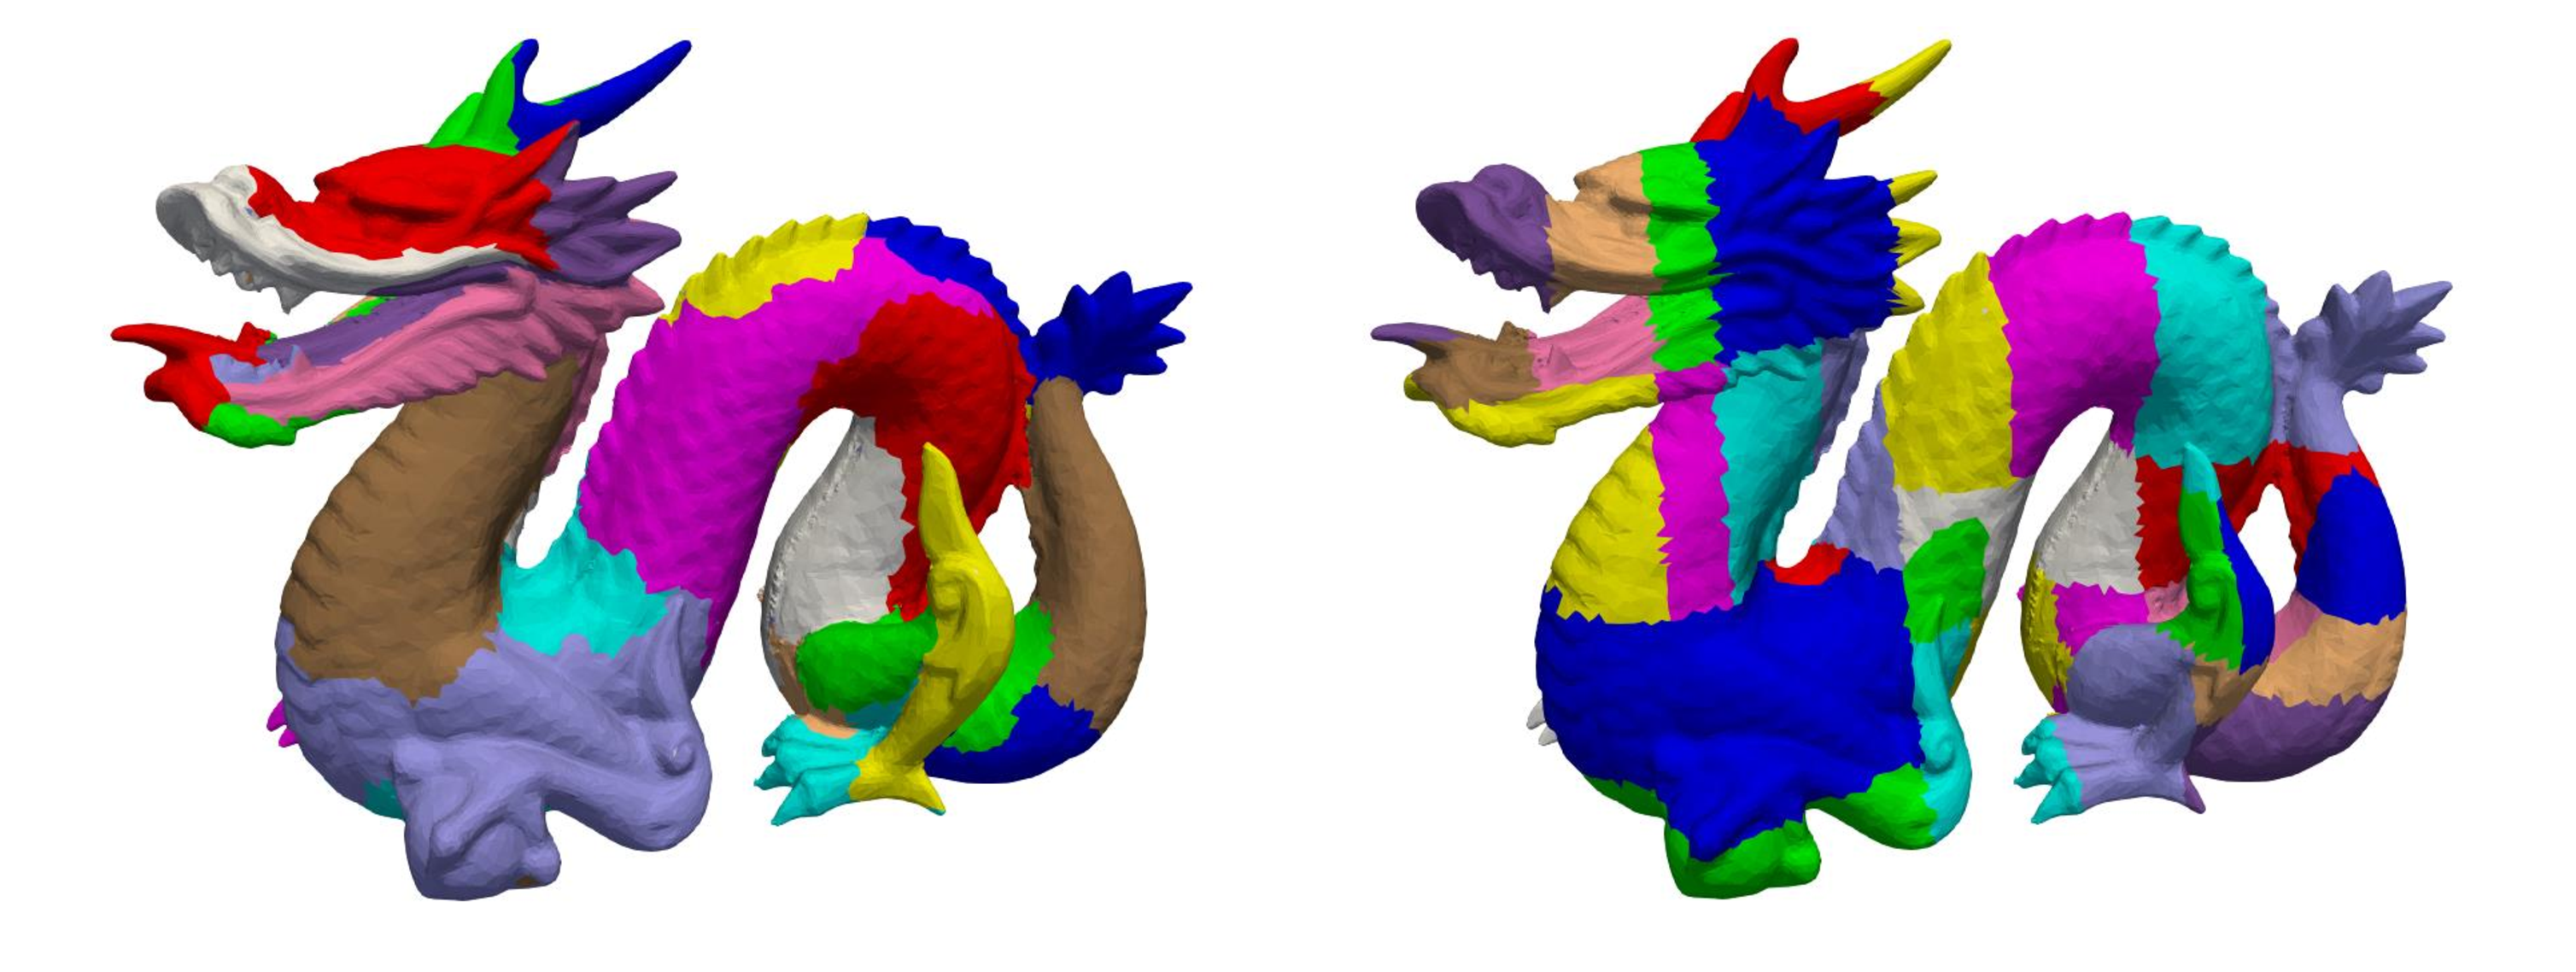
\includegraphics[width=1.0\textwidth]{fig/par_dragon_decomp.pdf}
\singlespacing
\captionstyle{center}\caption{Визуализация декомпозиции тестовой расчетной сетки dragon на 32 домена с помощью алгоритма Фархата (слева) и иерархического деления доменов (справа).}
\label{fig:text_2_smooth_decomp}
\end{figure}

\begin{figure}[!ht]
\centering
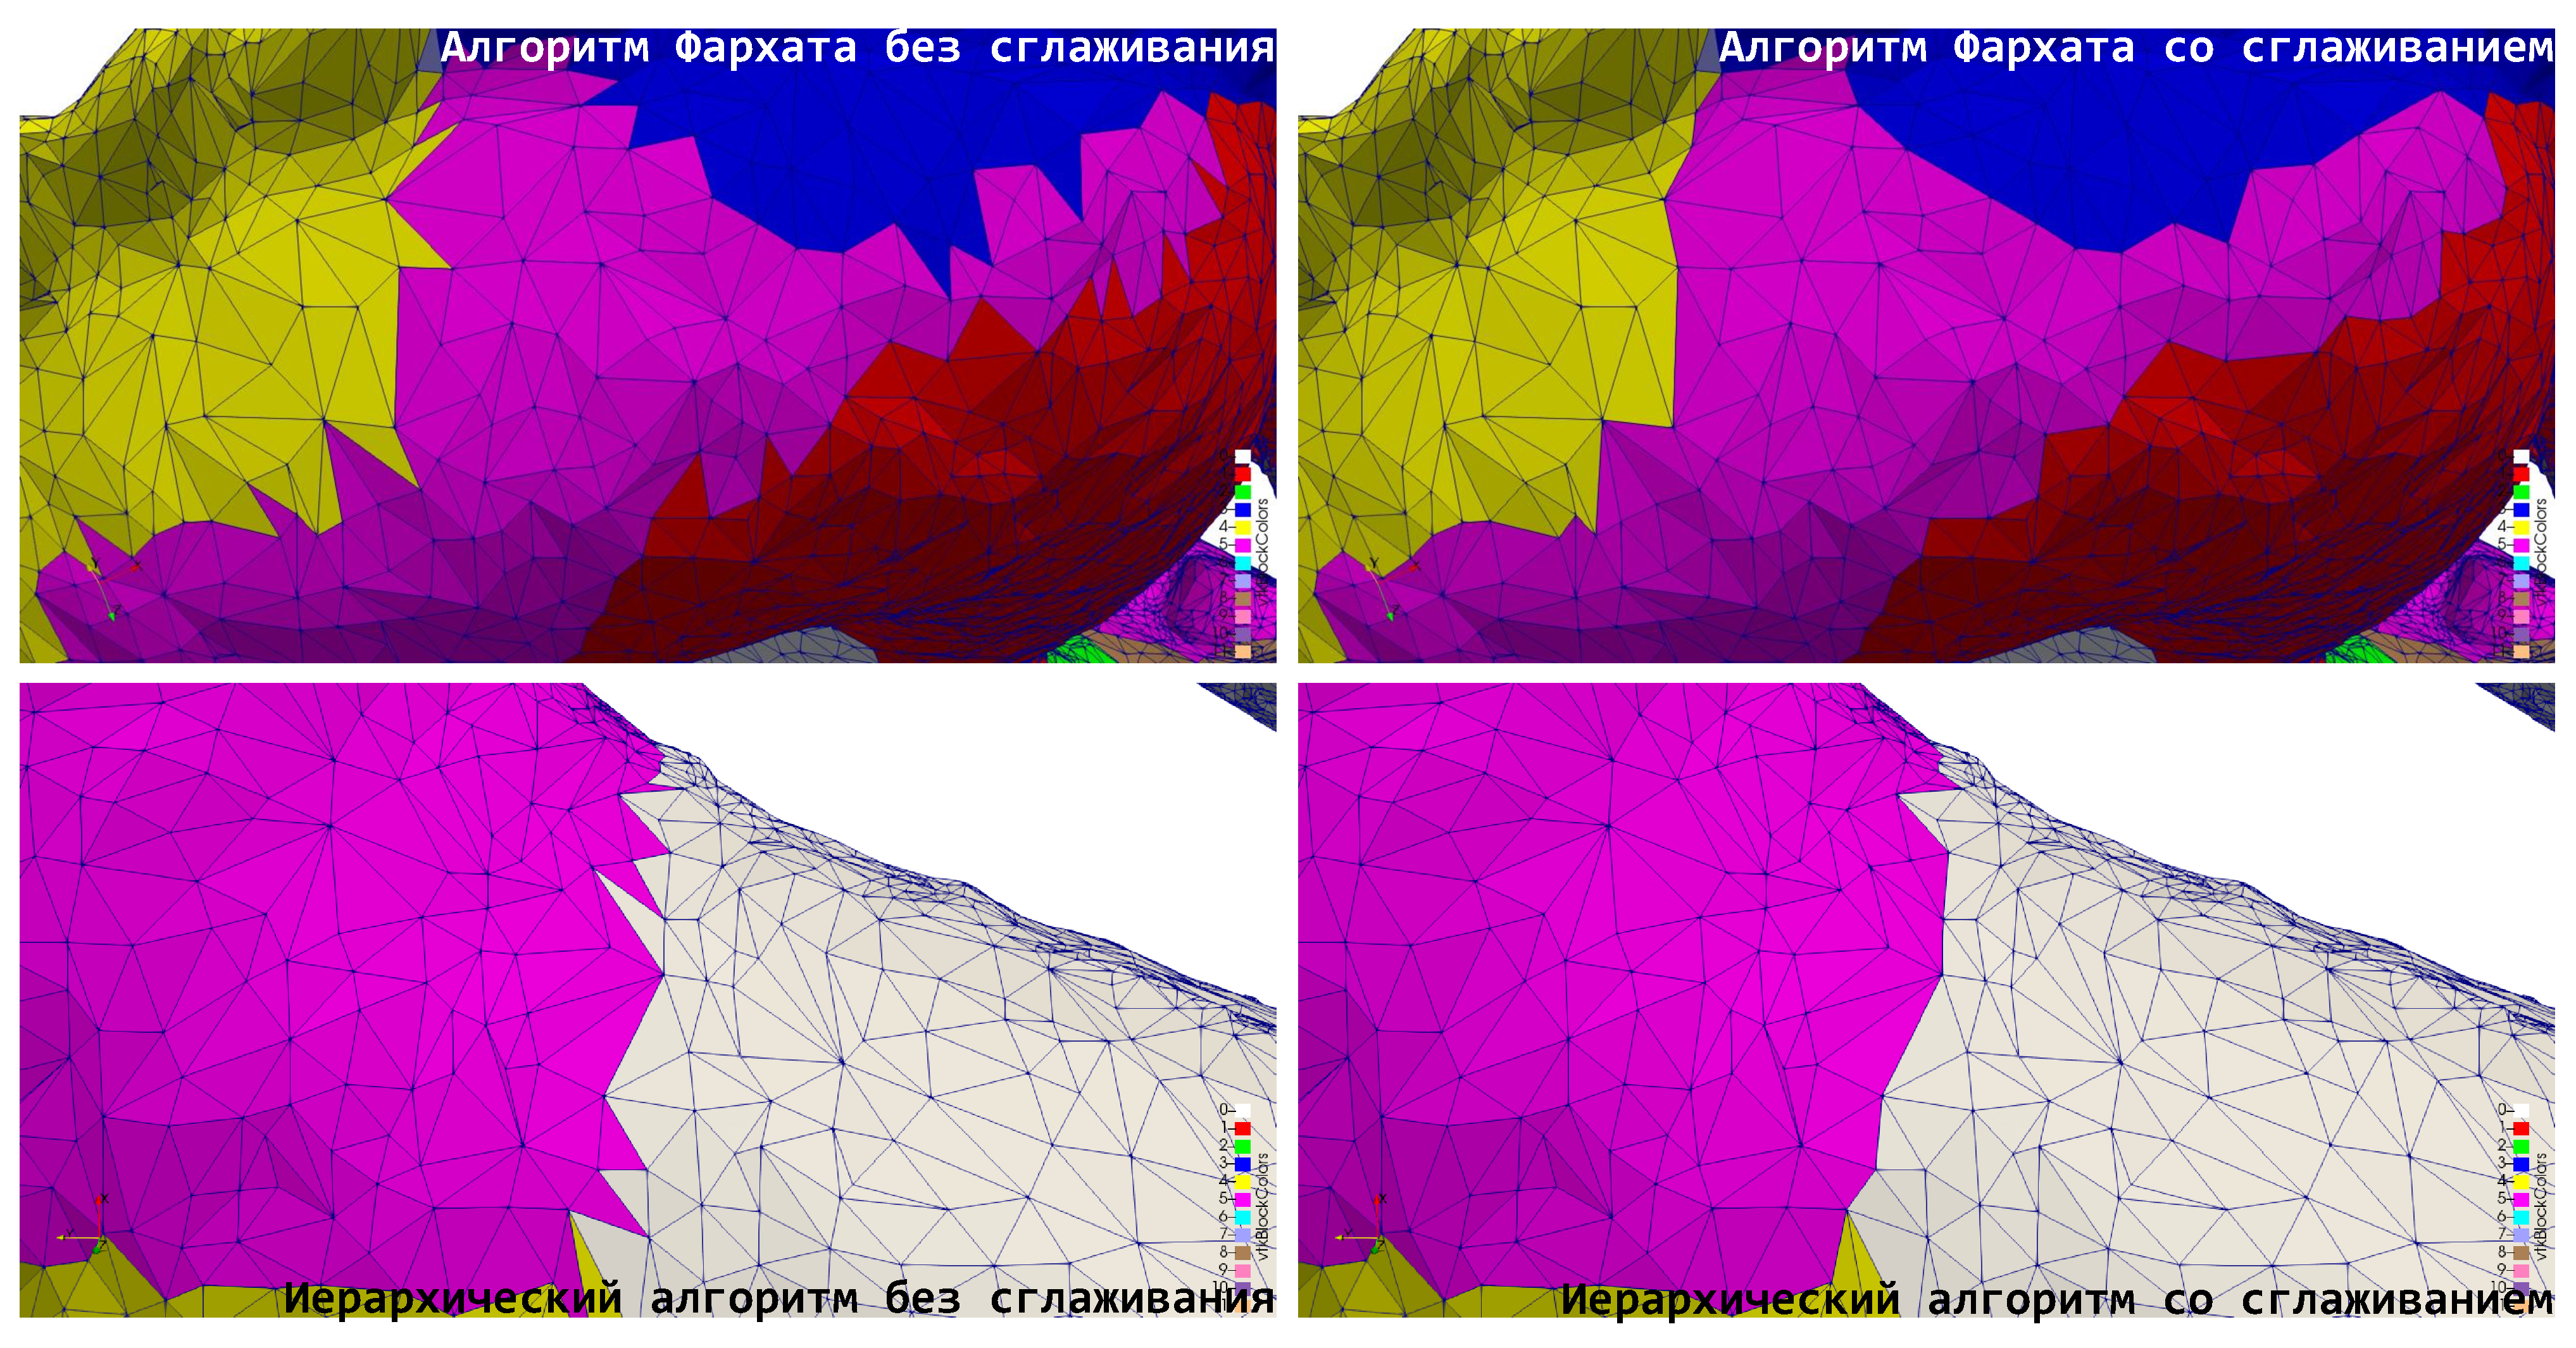
\includegraphics[width=0.9\textwidth]{fig/par_dragon_decomp2.pdf}
\singlespacing
\captionstyle{center}\caption{Визуализация применения сглаживания границ между доменами после работы алгоритма Фархата (сверху) и иерархического деления доменов (снизу).}
\label{fig:text_2_smooth_decomp2}
\end{figure}

На рис.~\ref{fig:text_2_smooth_decomp} представлена визуализация декомпозиции тестовой расчетной сетки dragon \cite{StanfordModels} с помощью алгоритма Фархата и иерархического деления доменов.
В обоих случаях декомпозиция выполнятся на 32 домена.
При этом на рис.~\ref{fig:text_2_smooth_decomp2} представлены результаты работы с уже примененным сглаживанием границ между доменами.
На рис.~\ref{fig:text_2_smooth_decomp2} крупным планом продемонстрированы отдельные части тестовой расчетной сетки dragon с отображением ребер ячеек.
На этом рисунке виден эффект от применения алгоритма сглаживания границ меду доменами, прежде всего от заключается в устранении одиноких ячеек, которые вторгаются в соседний домен одной своей вершиной.
После применения алгоритма границы между доменами визуально выглядят более гладко, их длина уменьшается.

Для тестирования эффективности алгоритма сглаживания границ между доменами использовались тестовые неструктурированные поверхностные сетки bunny (количество ячеек $5 \cdot 10^3$), dragon (количество ячеек $10^5$), lucy (количество ячеек $10^5$) \cite{StanfordModels}, к которым были применены алгоритмы декомпозиции с показателем $D = 0$ и сравнены показатели качества декомпозиции до и после сглаживания границ между доменами.
Результаты проведения экспериментов представлены на рис.~\ref{fig:text_2_smooth_graphics}.

\begin{figure}[H]
\centering
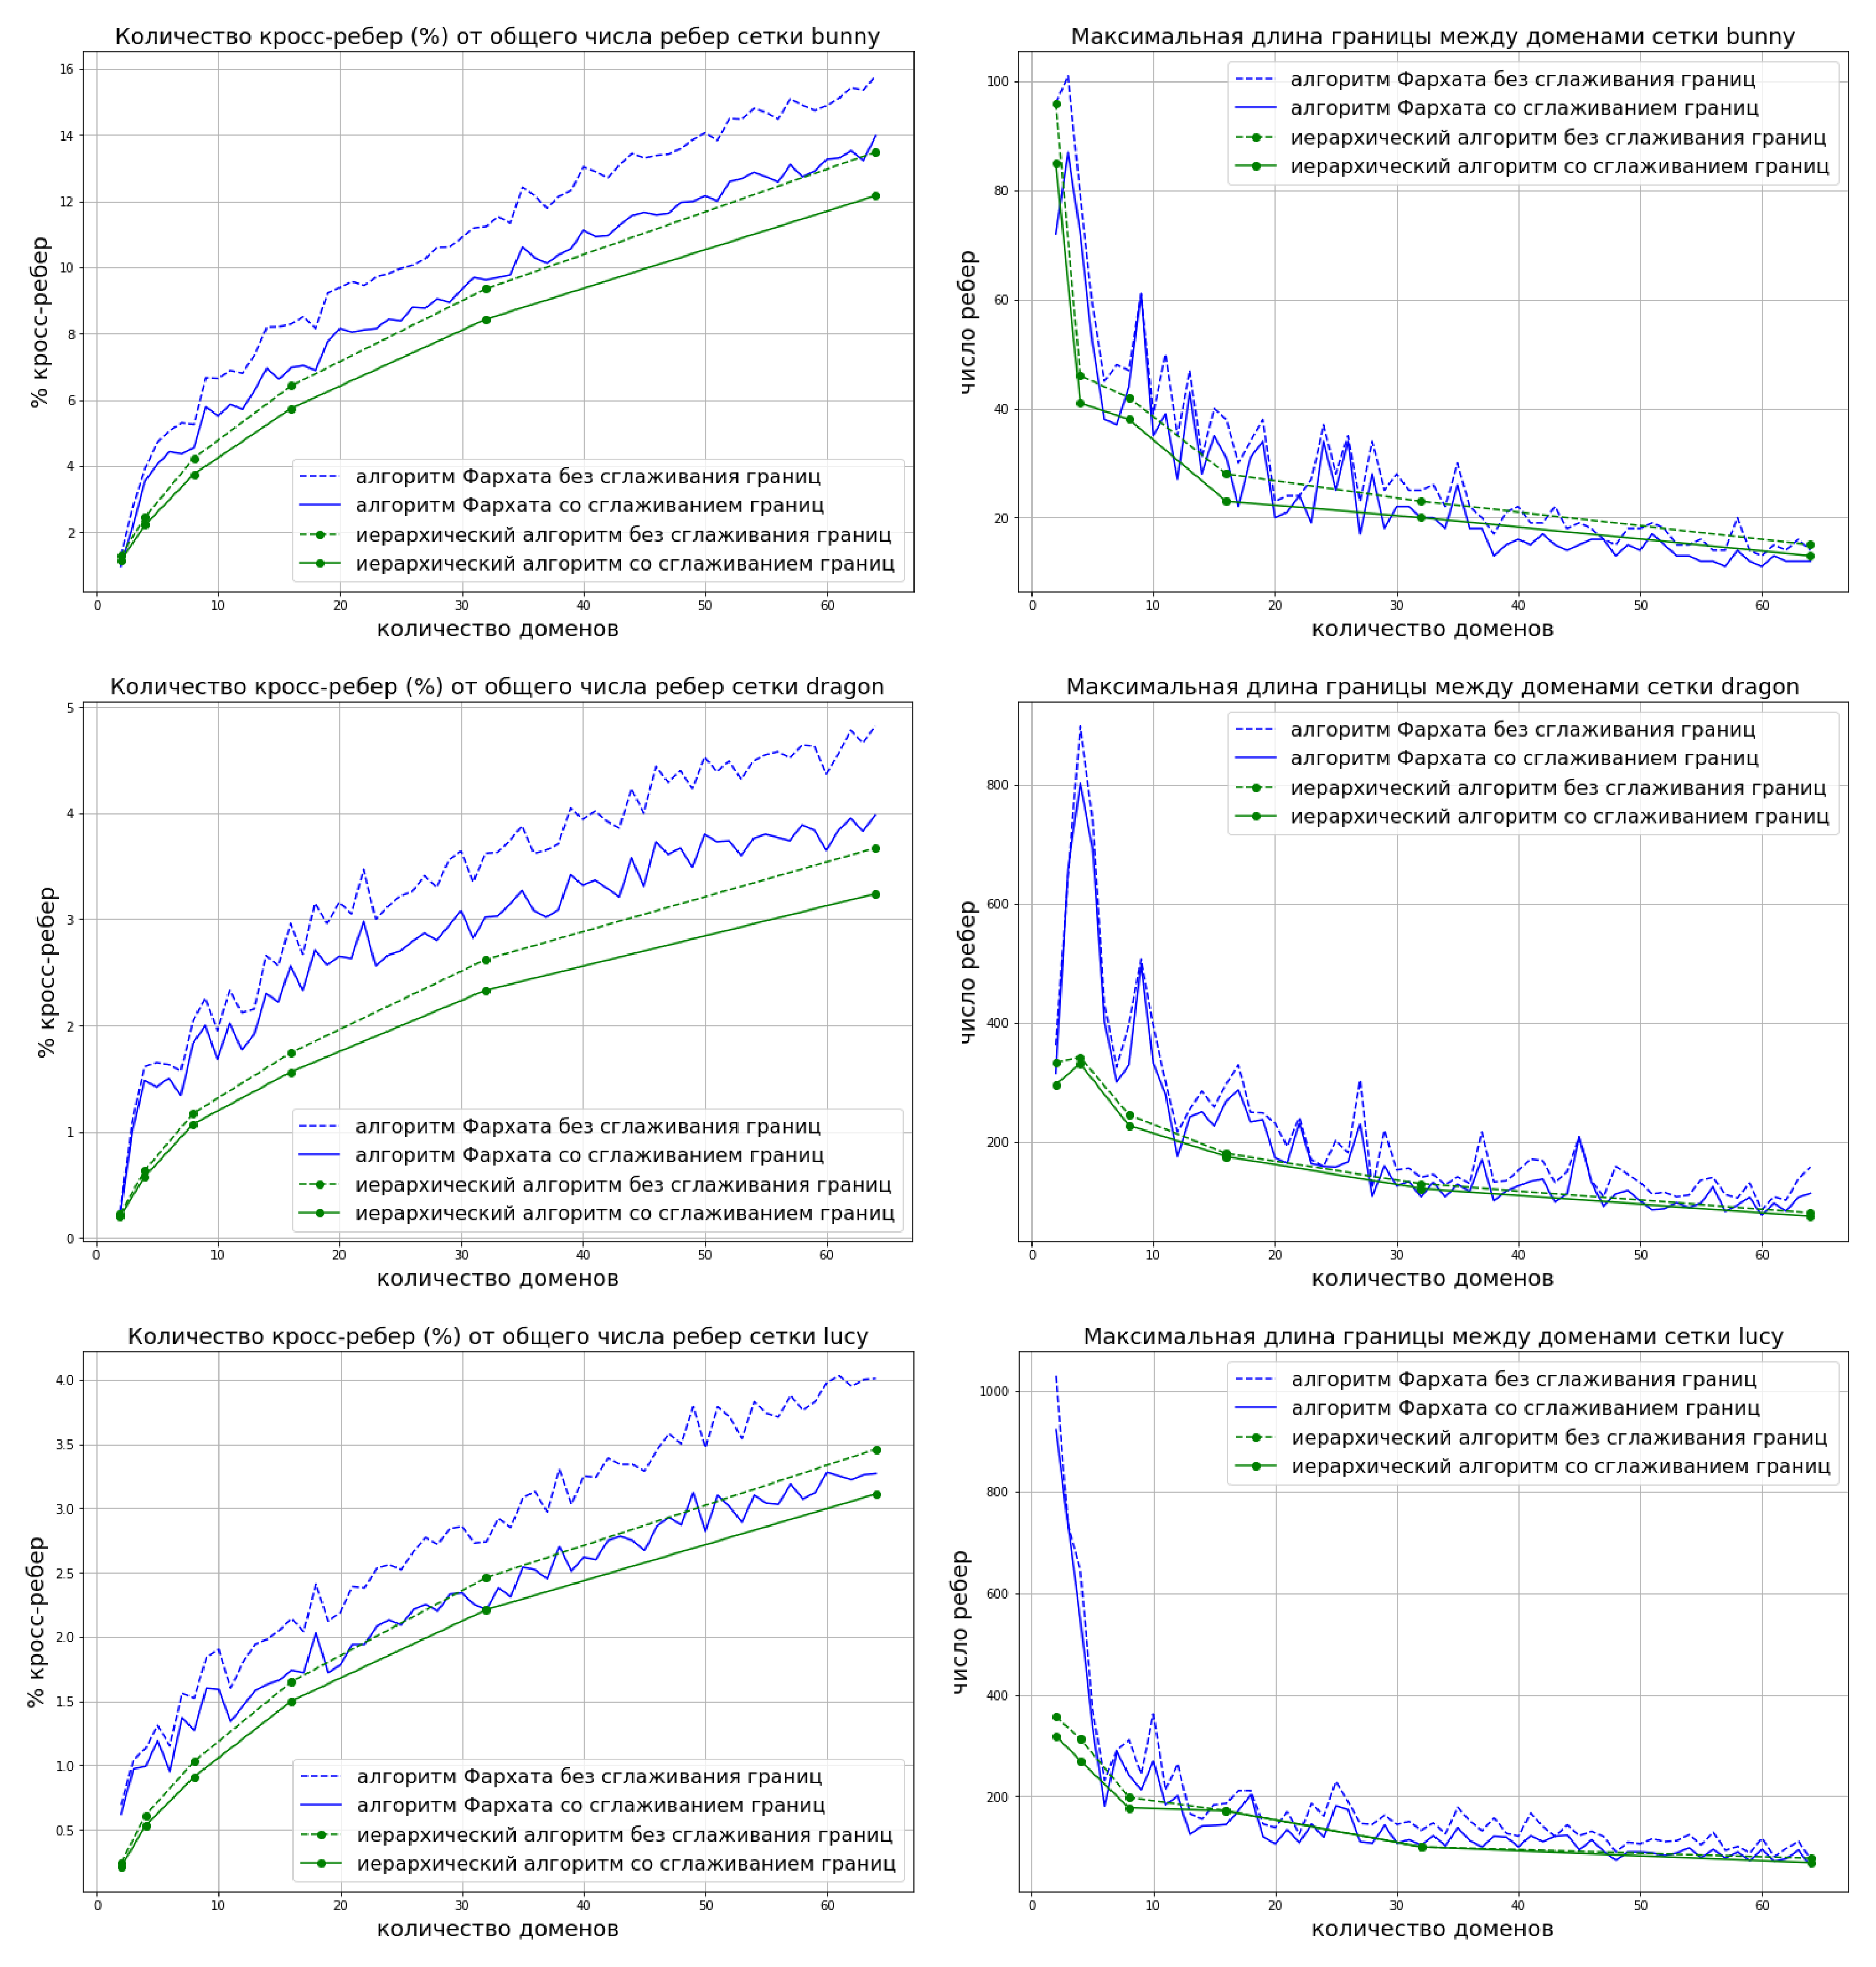
\includegraphics[width=1.0\textwidth]{fig/par_smooth_graphics.pdf}
\singlespacing
\captionstyle{center}\caption{Графики доли кросс-ребер от общего числа ребер сетки (показатель $I^{\%}$) и максимальной длины границы между доменами (показатель $L$) при декомпозиции тестовых сеток bunny, dragon и lucy на количество доменов от 2 до 64.}
\label{fig:text_2_smooth_graphics}
\end{figure}

Из приведенных на рис.~\ref{fig:text_2_smooth_graphics} графиков видно, что в целом проиллюстрированные показатели эффективности декомпозиции расчетных сеток (процентная доля ребер сетки, являющихся граничными ребрами между доменами, и максимальная длина границы между доменами) лучше для алгоритма иерархического деления доменов с выбором наилучшего направления в пространстве ($X$, $Y$, $Z$).
Применение же алгоритма сглаживания границ приводит к сокращению как общего количества граничных ребер (кросс-ребер), так и длины максимальной границы примерно на 10\%.
Этот эффект приводит к снижению времени межпроцессных обменов для задач, выполняющих расчеты на поверхностных расчетных сетках.

% Масштабирование вычислений на суперкомпьютере.
\subsubsection{Масштабирование вычислений на поверхностной расчетной сетке}

При проведении расчетов на декомпозированной сетке на каждой итерации счета необходимо выполнять обмен данными на каждой границе между доменами.
В нашем случае при выполнении декомпозиции расчетной сетки граница между двумя доменами представлена произвольным набором междоменных ребер.
При этом граница может быть разрывной, она и вовсе может состоять из отдельных ребер, поэтому последовательность междоменных ребер при описании границы не имеет значения.

На рис.~\ref{fig:text_2_scaling_mpi} представлена схема организации межпроцессных обменов.
На этой иллюстрации два домена (будем условно их называть левым и правым), обрабатывающиеся в MPI-процессах\label{abbr:mpi-5} с номерами 0 и 1, разделены границей, состоящей из трех ребер.
При этом в левом домене присутствует три ячейки, которые примыкают к рассматриваемой границе, в правом домене таких ячеек только две (так как ячейка 23R примыкает сразу к двум ребрам границы).
Для организации межпроцессных обменов в каждом домене для каждого ребра рассматриваемой границы создаются фиктивные ячейки, которые участвуют при расчете потоков через ребра границы.
При этом пересчет физических величин в фиктивных ячейках выполнять не требуется, все данные для фиктивных ячеек получаются с помощью MPI-обменов из настоящих ячеек соседнего домена.

\begin{figure}[ht]
\centering
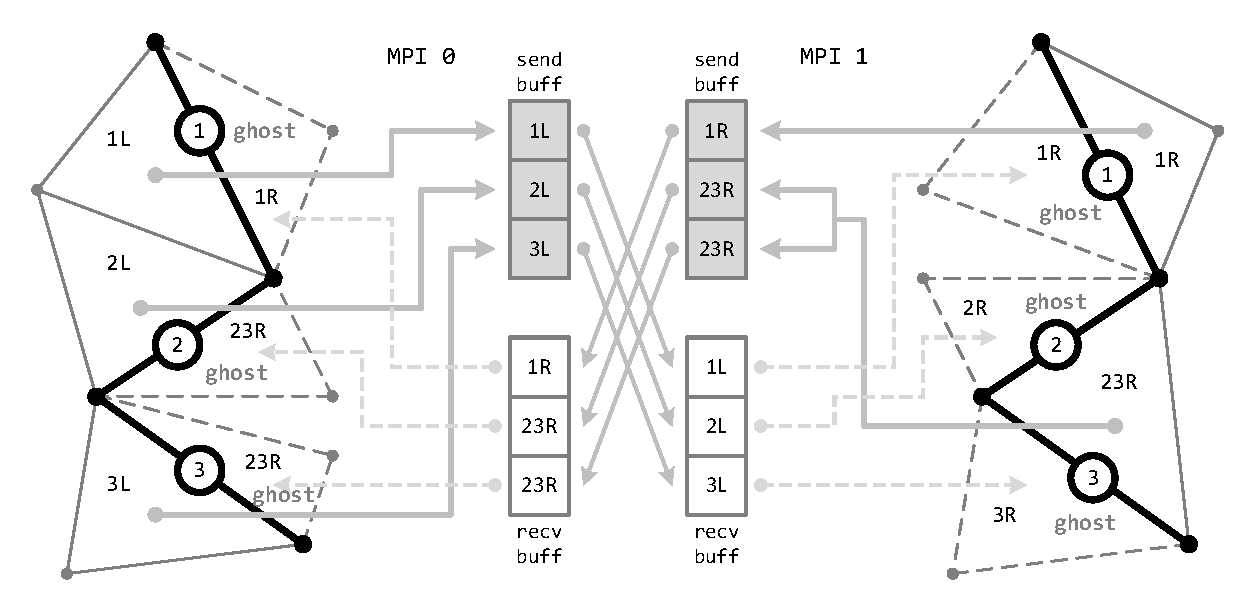
\includegraphics[width=1.0\textwidth]{fig/par_surf_mpi.pdf}
\singlespacing
\captionstyle{center}\caption{Схема выполнения MPI-обменов через границу двух доменов.}\label{fig:text_2_scaling_mpi}
\end{figure}

Для пересылки данных из настоящих граничных ячеек домена в фиктивные ячейки соседнего домена в каждом из двух соседних доменов организуются буферы отправки и приема данных.
Последовательность обмена данными выглядит следующим образом (схема показана на рис.~\ref{fig:text_2_scaling_mpi}).
Сначала данные из настоящих граничных ячеек записываются в соответствующие буферы отправки данных (send buff), далее для всех границ расчетной сетки выполняются асинхронные команды \texttt{MPI\_Irecv} приема сообщений в буферах получения данных (recv buff).
После чего также одновременно для всех границ расчетной сетки выполняются команды асинхронной отправки данных \texttt{MPI\_Isend} из буферов отправки.
Далее выполняется ожидание завершения всех асинхронных обменов данными с помощью функции \texttt{MPI\_Waitall}.
Последним шагом, завершающим обмен данными между соседними доменами, является перенос полученных физических значений из буферов получения данных (recv buff) в соответствующие фиктивные ячейки.

Можно отметить, что при использовании фиктивных ячеек возможно некоторое дублирование данных.
Например, на представленной схеме ячейке 23R из правого домена соответствуют сразу две фиктивные ячейки в левом домене.
Эти ячейки содержат одинаковые данные.
Такое дублирование информации является приемлемым, так как данные фиктивных ячеек используются только на чтение для выполнения вычисления потоков через границу доменов, поэтому выполнять какую-либо синхронизацию одинаковых фиктивных ячеек не нужно.

Для замеров показателей масштабируемости вычислений на неструктурированной поверхностной расчетной сетке была использована тестовая поверхность обтекаемого трехмерного тела, содержащая порядка $2 \cdot 10^5$ узлов и $4 \cdot 10^5$ ячеек.
В ячейках выполнялись расчеты, связанные с моделированием течения жидкой пленки, решением уравнений теплового баланса на поверхности, а также перестроение и сглаживание поверхности.
Для декомпозиции поверхностной сетки использовался простой иерархических алгоритм деления доменов пополам из раздела~\ref{sec:text_2_decompsurf_hierarchical}, в котором в качестве признаков ячеек брались три координаты центра, а критерием выбора конкретной координаты для деления домена являлась минимизация длины границы между двумя доменами.
К результату декомпозиции был применен алгоритм сглаживания границ между доменами из раздела~\ref{sec:text_2_smooth}.

\begin{table}[!ht]
\centering
\setcaptionmargin{0mm}
\onelinecaptionsfalse
\singlespacing
\captionstyle{center}\caption{Конфигурации узлов суперкомпьютера МВС-10П, на которых производились замеры масштабирования вычислений.}
\bigskip
\begin{tabular}{|c|c|c|c|c|}
\hline
\makecell{Семейство \\
процессоров \\
Intel} & \makecell{Количество\\процессоров\\/ ядер\\/ потоков} & \makecell{Частота\\процессора} & \makecell{Объем\\оперативной\\памяти} & \makecell{AVX-512\label{abbr:avx-1}} \\
\hline\hline
Haswell & 2 / 28 / 56 & 2,6 ГГц & 128 ГБ & нет \\
\hline
Broadwell & 2 / 32 / 64 & 2,6 ГГц & 128 ГБ & нет \\
\hline
Phi KNL\label{abbr:knl-2} & 1 / 72 / 288 & 1,5 ГГц & 96 ГБ & да \\
\hline
Skylake & 2 / 36 / 72 & 3,0 ГГц & 192 ГБ & да \\
\hline
Cascade Lake & 2 / 48 / 96 & 3,0 ГГц & 192 ГБ & да \\
\hline
\end{tabular}
\label{tbl:text_2_scaling_supercomputers}
\end{table}   

Для измерения показателей масштабируемости вычислений использовались гомогенные сегменты вычислительной системы МВС-10П.
Всего расчеты проводились на четырех вычислительных сегментах, характеристики узлов которых приведены в таблице~\ref{tbl:text_2_scaling_supercomputers} (использовались все приведенные узлы кроме Haswell) \cite{Shabanov2021Scaling}.
В этой таблице можно отметить, что все микропроцессоры кроме Intel Xeon Broadwell поддерживают набор инструкций AVX-512, позволяющий использовать специальные 512-битные векторные регистры для эффективной векторизации кода.
Также следует выделить вычислительные узлы на базе микропроцессора Intel Xeon Phi KNL.
Эти микропроцессоры отличаются большим количеством вычислительных ядер, каждое из которых способно выполнять до 4 потоков, что позволяет эффективно распараллеливать расчетные приложения вплоть до 288 потоков на одном микропроцессоре.

\begin{figure}[ht]
\centering
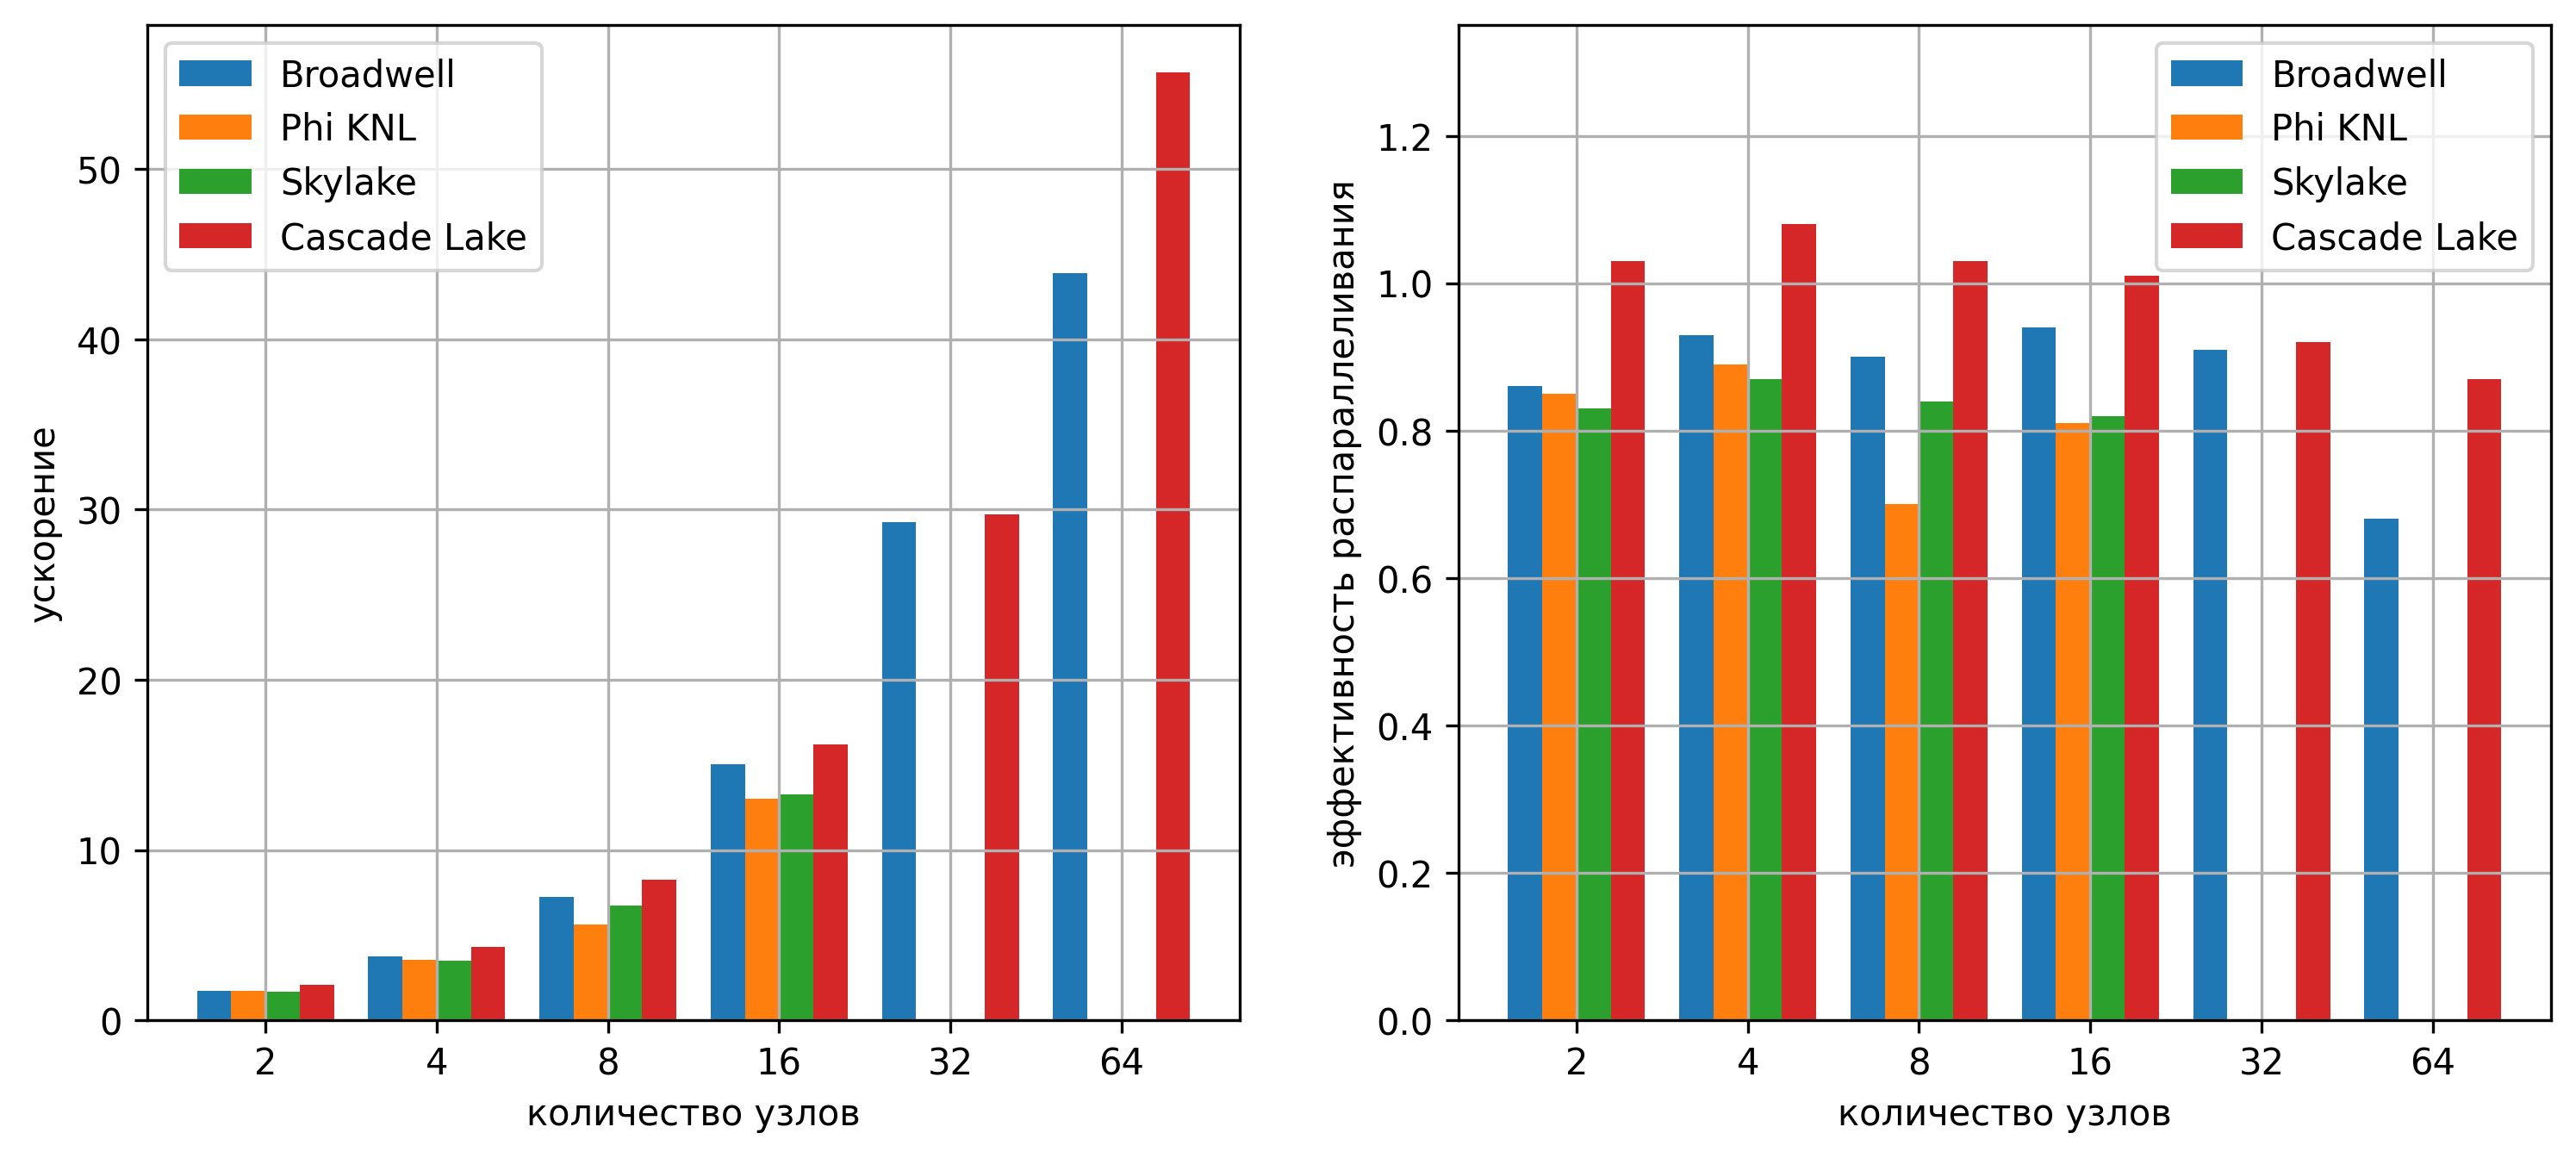
\includegraphics[width=1.0\textwidth]{fig/par_surf_2in1.png}
\singlespacing
\captionstyle{center}\caption{Ускорение (слева) и эффективность распараллеливания (справа) вычислений на сегментах суперкомпьютера МВС-10П при увеличении количества узлов.}
\label{fig:text_2_scaling_speedup_eff}
\end{figure}

Основной целью выполняемых запусков было проведение замеров показателей сильной масштабируемости вычислений при полном распараллеливании внутри вычислительных узлов с использованием OpenMP.
То есть для всех запусков использовалась одна и та же поверхностная расчетная сетка (которая дробилась на нужное количество вычислительных процессов), также в расчетах были задействованы все потоки, доступные внутри вычислительных узлов.

При проведении расчетов замеры выполнялись независимо для каждой вычислительной системы в отдельности.
На рис.~\ref{fig:text_2_scaling_speedup_eff} приведены диаграммы ускорения вычислений $s_{msg}$ и эффективности распараллеливания $e_{msg}$ при увеличении количества вычислительных узлов для разных вычислительных систем.
Можно видеть, что для всех вычислительных систем эффективность масштабирования варьируется в районе значений 0,8-0,9, хотя на некоторых конфигурациях запуска наблюдаются провалы даже в район 0,7.
Запуски с низким значением эффективности распараллеливания как правило связаны с разбросом времени обработки MPI\label{abbr:mpi-6} процессами своих доменов.
Заметим, что для сегмента Cascade Lake при количестве узлов 2, 4, 8 и 16 наблюдается проявление сверхлинейной масштабируемости (когда значение $e_{msg}$ поднимается выше единицы), однако это скорее исключение, чем ожидаемый эффект.

%---------------------------------------------------------------------------------------------------
% 4.4 - общая память

\subsection{Методы распараллеливания на общей памяти}

В предыдущих разделах были рассмотрены вопросы, касающиеся распараллеливания вычислений между отдельными узлами суперкомпьютера и запущенными на них процессами.
Современные микропроцессоры, входящие в состав вычислительных узлов, содержат десятки вычислительных ядер \cite{Section3IntroIntel,Section3IntroAMD,Kuzminsky2022ARM}, что с учетом многопоточности приводит необходимости организации вычислений в рамках одного узла с использованием сотен потоков, работающих на общей памяти.

Так же как и в случае распределения вычисления между узлами суперкомпьютера распараллеливание вычислений на общей памяти преследует цель сокращения времени выполнения приложений.
Исходя из этого основным показателем качества организации высокопроизводительных вычислений на общей памяти является ускорение выполнения задачи при увеличении количества задействованных потоков.

\begin{definition}
Ускорением выполнения задачи в модели распараллеливания на общей памяти при использовании $k$ потоков будем называть величину $s_{shr}(k) = \frac{T(1)}{T(k)}$, где $T(i)$ -- время выполнения задачи с использованием $i$ потоков.
\end{definition}

\begin{definition}
Эффективностью распараллеливания при выполнении задачи на общей памяти при использовании $k$ потоков будем называть величину $e_{shr}(k) = \frac{s_{shr}(k)}{k}$.
\end{definition}

Параметры $s_{shr}$ и $e_{shr}$ аналогичны параметрам ускорения и эффективности распараллеливания вычислений в модели с передачей сообщений.
В случае идеального распараллеливания вычислений $s_{shr}(k) = k$, $e_{shr}(k) = 1$.

Основной проблемой снижения эффективности распараллеливания вычислений на общей памяти являются конфликты при доступе разных потоков к одной и той же области данных.
В этой главе рассмотрены вопросы организации вычислений на поверхностной неструктурированной расчетной сетке на общей памяти с целью устранения конфликтов по данным между разными потоками.

Во время выполнения расчетов на поверхностной неструктурированной сетке при обработке ячейки необходимо обращаться за данными к ее вычислительной окрестности, которая в простейшем случае представляет собой все соседние по ребрам ячейки.
Аналогично, все ячейки из окрестности обращаются к рассматриваемой ячейке, и при одновременном обращении к каким-либо данным на запись возникает конфликт между потоками, обрабатывающими разные ячейки окрестности.
Добиться устранения таких конфликтов можно путем запрета параллельной обработке ячеек, принадлежащих к вычислительно окрестности одной и той же ячейки.
Эта задача напрямую связана с задачей реберной раскраски дуального графа расчетной сетки, в результате которой множество ребер разбиваются на подмножества, не содержащие конфликтующих ребер.

\subsubsection{Распараллеливание вычислений на общей памяти для задачи обледенения}\label{sec:text_3_edge_coloring}

Будем рассматривать проблему распараллеливания вычислений на общей памяти применительно к задаче расчета обледенения поверхности с помощью конечно-объемного метода \cite{Gulicheva2024}.
Моделирование процесса обледенения поверхности тела выполняется итерационно.
На каждой итерации расчетов в каждой расчетной ячейке производится решение системы уравнений массового и теплового балансов, из которой получаются основные данные состояния расчетной ячейки (температура, количество жидкой воды и накопленного льда и другие).
Между расчетными итерациями выполняется расчет протекания потоков жидкости между соседними ячейками (потоки массы и тепла через границы ячеек).
Также в зависимости от настроек решателя через заданные промежутки времени выполняется пересчет геометрии поверхности тела за счет накопленной в ее ячейках массы льда.
Расчеты обледенения выполняются на неструктурированной поверхностной расчетной сетке с треугольными ячейками.

\begin{lstlisting}[caption={Расчет протекания потоков через ребро сетки.}, label={lst:text_3_flows_through_edge}]
void Edge::calc_flows()
{
    // cells pair
    Cell* fst = ...;
    Cell* sec = ...;

    // flows calculation
    double flow_w = ...;
    double flow_q = ...;

    // flows correction
    fst->flow_out_w += flow_w;
    fst->flow_out_q += flow_q;
    sec->flow_out_w -= flow_w;
    sec->flow_out_q -= flow_q;
}
\end{lstlisting}

Пересчет состояния ячейки выполняется независимо от других ячеек, данные вычисления могут выполняться параллельно.
Пересчет потоков массы и тепла выполняются через каждое ребро расчетной сетки, при этом поток перетекает из одной инцидентной ребру ячейки в другую.
Общая схема пересчета потоков для одного ребра может выглядеть так, как представлено на листинге~\ref{lst:text_3_flows_through_edge}.

Для выполнения пересчета потоков для всех ребер домена расчетной сетки необходимо обработать все ребра в цикле (см. листинг~\ref{lst:text_3_flows_through_edges}).

\begin{lstlisting}[caption={Расчет протекания потоков для всех ребер домена.}, label={lst:text_3_flows_through_edges}]
for (auto e : own_edges)
{
    e->calc_flows();
}
\end{lstlisting}

При обработке ребер домена расчетной сетки в цикле возникает желание распараллелить или векторизовать этот цикл.
При распараллеливании вычислений с помощью OpenMP следует учитывать конфликты по данным, которые могут возникнуть при выполнении корректировки потоков (в случае если несколько потоков начнут одновременно изменять значение одной области памяти).
Для устранения этих конфликтов достаточно выполнять операции корректировки потоков в атомарном режиме, как показано на листинге~\ref{lst:text_3_atomic_flows}.

\begin{lstlisting}[caption={Атомарные операции корректировки потоков.}, label={lst:text_3_atomic_flows}]
#pragma omp atomic
fst->flow_out_w += flow_w;
#pragma omp atomic
fst->flow_out_q += flow_q;
#pragma omp atomic
sec->flow_out_w -= flow_w;
#pragma omp atomic
sec->flow_out_q -= flow_q;
\end{lstlisting}

Использование \texttt{\#pragma omp atomic} гарантирует, что указанная команда одновременно будет обрабатываться только одним потоком (то есть, что между чтением старого значения переменной и записью нового значения не попадут операции другого потока).
При большом количестве используемых потоков это может приводить к потерям производительности.

\subsubsection{Сведение задачи распараллеливания вычислений к реберной раскраске}

Будем решать задачу разрешения конфликтов между ребрами расчетной сетки с помощью реберной раскраски графа конфликтов.
Такой подход является достаточно естественным \cite{Gilfanov2021Coloring}, и в нашем случае вершины графа конфликтов будут иметь низкую степень, что свидетельствует о допустимости реберной раскраски в небольшое количество цветов.

Рассмотрим ситуацию, при которой возможно возникновение конфликта при корректировке потоков во время параллельной обработки двух ребер расчетной сетки.
Такой конфликт возможен в том случае, когда оба обрабатываемых ребра являются инцидентными одной и той же ячейке.
Рассмотрим дуальный граф нашей расчетной сетки.
Без ограничения общности будем считать, что рассматриваемая расчетная сетка не имеет краев, то есть каждая ее ячейка имеет ровно трех соседей.
В этом случае ее дуальный граф будет кубическим.
При этом задача разбиения ребер расчетной сетки на неконфликтующие множества сводится к построению реберной раскраски дуального графа.
В процессе нахождения реберной раскраски построенного дуального графа зададимся вопросом, вызывающим  исследовательский интерес -- в какое минимальное количество цветов можно раскрасить этот граф.
При этом будем считать, что мы рассматриваем только односвязные поверхности.
Таким образом, анализируемых дуальный граф является плоским кубическим графом.
Также отметим, ни одна расчетная ячейка исходной сетки не может быть соседней себе самой, а значит в построенном дуальном графе нет мостов.
То есть объектом нашего исследования является плоский кубический граф без мостов.

\subsubsection{Реберная раскраска в 5 и 4 цвета}

Алгоритмы раскраски плоского кубического графа без мостов в 5 и 4 цветов являются достаточно тривиальными, рассмотрим их.

\begin{lemma}\label{lem:text_3_graph_prim_coloring5}
Кубический граф допускает реберную раскраску в $5$ цветов, и эта раскраска может быть построена с линейной сложностью по количеству ребер.
\end{lemma}
Для построения требуемой раскраски достаточно последовательно перебрать все ребра.
Так как для каждого ребра существует ровно $4$ смежные ребра, то из пяти цветов всегда можно выбрать цвет, в который не покрашено ни одно из этих смежных ребер.
Таким образом, раскраска строится за один проход по всем ребрам, то есть с линейной сложностью.
$\blacksquare$\\

В лемме~\ref{lem:text_3_graph_prim_coloring5} не использовалась планарность графа, а количество цветов явно избыточно.
Согласно теореме Визинга \cite{Vizing1964,Vizing1965} кубический граф допускает реберную раскраску в $4$ цвета.
Однако, теорема Визинга также не использует планарность графа, и алгоритм, построенный исходя из доказательства, будет иметь сложность, выше линейной по количеству ребер \cite{Soifer2009}.
Приведем альтернативное доказательство с использованием планарности графа и более низкой сложностью алгоритма построения реберной раскраски в $4$ цвета.

\begin{lemma}\label{lem:text_3_graph_prim_coloring4}
Кубический граф допускает реберную раскраску в $4$ цвета, и эта раскраска может быть построена с линейной сложностью по количеству ребер.
\end{lemma}

Доказательство существования раскраски будем проводить по индукции по количеству вершин графа.
База индукции: кубический граф с минимальным количеством вершин это $K_4$.
Для этого графа утвержление очевидно.

Предположим, что утверждение теоремы верно для всех кубических графов с порядок которых изменяется от $4$ до $n - 2$ (отметим, что порядок кубического графа не может быть нечетным).

Рассмотрим кубический планарный граф, с множеством вершин $V$ ($n = |V| = \nu$), множеством ребер $E$ ($|E| = \varepsilon$) и множеством граней $F$ ($|F| = \zeta$).
При этом внешнюю область вокруг графа также считаем гранью (рассматриваем граф, расположенный на сфере).
Также через $\zeta_i$ обозначим количество граней, содержашей ровно $i \ge 3$ вершин (в этом случае будем говорить, что грань имеет размер $i$).
\begin{equation}
	\zeta = \sum_{i = 3}^{\infty}{\zeta_i}.
\end{equation}
Рассмотрим соотношения, выполняемые для этого графа.

Так как степень каждой вершины равна $3$, то лемма о рукопожатиях для этого графа приобретает вид
\begin{equation}
	3 \nu = 2 \varepsilon.
\end{equation}

Так как каждое ребро входит ровно в две грани, то верно соотношение
\begin{equation}
	2 \varepsilon = \sum_{i = 3}^{\infty}{i \zeta_i}.
\end{equation}

Наконец, для рассматриваемого графа выполняется соотношение Эйлера $\nu + \zeta - \varepsilon = 2$.
Подставив в соотношение Эйлера выражения для $\nu$, $\zeta$ и $\varepsilon$ получим
\begin{equation}
	2 \cdot 2\varepsilon + 6 \sum_{i = 3}^{\infty}{\zeta_i} - 3 \cdot 2\varepsilon = 12
\end{equation}
\begin{equation}
	6 \sum_{i = 3}^{\infty}{\zeta_i} - \sum_{i = 3}^{\infty}{i \zeta_i} = 12
\end{equation}
\begin{equation}\label{eqn:text_3_graph_prim_euler}
	\sum_{i = 3}^{\infty}{(6 - i) \zeta_i} = 12
\end{equation}

Из \eqref{eqn:text_3_graph_prim_euler} видно, что в рассматриваемом графе найдется грань размера $3$, $4$ или $5$.
Рассмотрим каждый этих случаев отдельно.

Случай 1. Сначала рассмотрим случай наличия в графе гамака, состоящего из двух треугольных граней, как показано на рис.~\ref{fig:text_3_graph_prim_coloring4_gamak} слева.

\begin{figure}[ht]
\centering
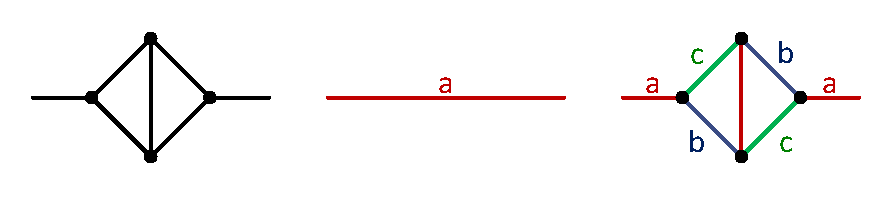
\includegraphics[width=1.0\textwidth]{fig/par_coloring4_gamak.pdf}
\singlespacing
\captionstyle{center}\caption{Случай наличия в графе гамака из двух треугольных граней.}
\label{fig:text_3_graph_prim_coloring4_gamak}
\end{figure}

Стянув гамак в одно ребро (рис.~\ref{fig:text_3_graph_prim_coloring4_gamak} в центре), получим граф с $n - 4$ вершинами, ребра которого могут быть раскрашены в 4 цвета по предположению индукции.
Тогда по этой раскраске не представляется сложным раскрасить исходный граф, как показано на рис.~\ref{fig:text_3_graph_prim_coloring4_gamak} справа.

Случай 2. В графе нет гамаков, состоящих из двух треугольных граней, но найдется треугольная грань (см. рис.~\ref{fig:text_3_graph_prim_coloring4_face3} слева).

\begin{figure}[ht]
\centering
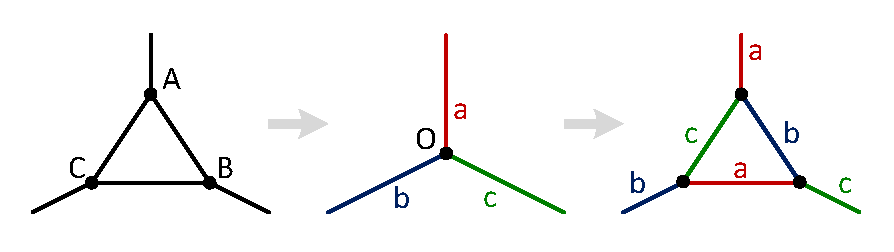
\includegraphics[width=1.0\textwidth]{fig/par_coloring4_face3.pdf}
\singlespacing
\captionstyle{center}\caption{Случай наличия в графе треугольной грани.}
\label{fig:text_3_graph_prim_coloring4_face3}
\end{figure}

Стянем треугольную грань $ABC$ в точку $O$, как показано на рис.~\ref{fig:text_3_graph_prim_coloring4_face3} в центре.
Так как в графе не было гамаков, состоящих из двух треугольных граней, то у грани $ABC$ не было соседних треугольных граней по ребру, а значит при стягивании $ABC \rightarrow O$ ни одна грань кроме $ABC$ не выродилась.
Это значит, что мы получили плоский кубический граф с $n - 2$ вершинами, ребра которого могут быть раскрашены в 4 цвета по предположению индукции.
Тогда по этой раскраске можно построить раскраску исходного графа, как показано на рис.~\ref{fig:text_3_graph_prim_coloring4_face3} справа.

Случай 3. В графе нет треугольных граней, но найдется четырехугольная грань (см. рис.~\ref{fig:text_3_graph_prim_coloring4_face4} слева).

\begin{figure}[ht]
\centering
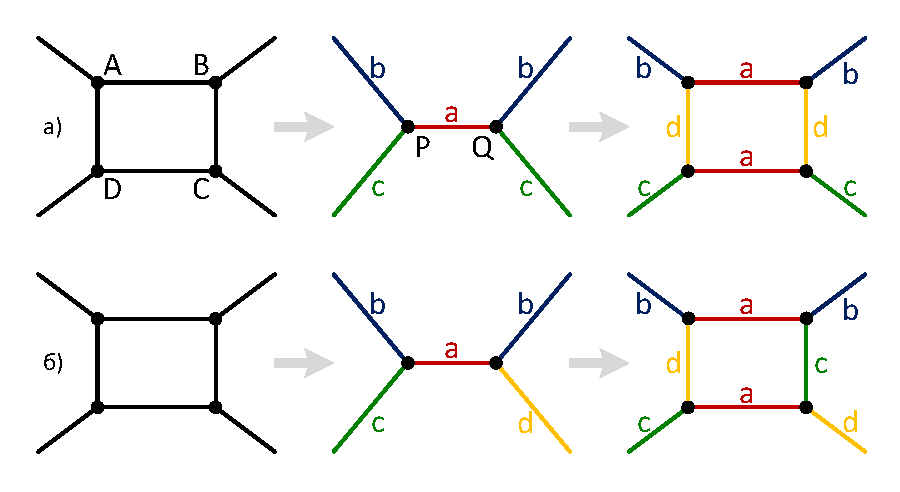
\includegraphics[width=1.0\textwidth]{fig/par_coloring4_face4.pdf}
\singlespacing
\captionstyle{center}\caption{Случай наличия в графе четырехугольной грани.}
\label{fig:text_3_graph_prim_coloring4_face4}
\end{figure}

Рассмотрим четырехугольную грань $ABCD$.
Выполним стягивание ребер $AD \rightarrow P$, $BC \rightarrow Q$.
Так как в графе не было треугольных граней, то при стягивании выродилась только грань $ABCD$.
Мы получили плоский кубический граф с $n - 2$ вершинами, ребра которого могут быть раскрашены в 4 цвета по предположению индукции.
По этой раскраске построим раскраску исходного графа.
Для этого перенесем цвета всех ребер (кроме $PQ$) на исходный граф, непокрашенными останутся только ребра цикла $A-B-C-D$.
Пусть $\gamma(PQ) = a$.
Если для покраски остальных 4 ребер, инцидентных вершинам $P$ и $Q$, были использованы только 2 цвета ($b$ и $c$), то исходный граф можно покрасить в 4 цвета, покрасив ребра цикла $A-B-C-D$ в цвета $a$ и $d$ (см. рис.~\ref{fig:text_3_graph_prim_coloring4_face4} сверху).
Если для покраски остальных 4 ребер, инцидентных вершинам $P$ и $Q$, были использованы все оставшиеся три цвета ($b$, $c$ и $d$), то одним из этих цветов было покрашено 2 ребра (пусть это будет цвет $b$), а двумя другими цветами -- по одному ребру (см. рис.~\ref{fig:text_3_graph_prim_coloring4_face4} снизу).
В этом случае раскрасим ребра цикла $A-B-C-D$ в цвета $a$, $c$, $d$ следующим образом.
К циклу $A-B-C-D$ примыкает одно ребро цвета $c$, оно смежно двум ребрам этого цикла (которые являются смежными между собой), которые не могут быть покрашены с цвет $c$.
То есть в циикле $A-B-C-D$ найдется пара смежных ребер, одно из которых может быть покрашено в цвет $c$ (обозначим эту пару $p_c$).
Аналогично, в цикле $A-B-C-D$ найдется пара смежных ребер, одно из которых может быть покрашено в цвет $d$ (обозначим эту пару $p_d$).
Вне зависимости от того пересекаются ли $p_c$ и $p_d$, в цикле $A-B-C-D$ можно найти такие несмежные ребра $e_c$ и $e_d$, что $e_c \in p_c$, $e_d \in p_d$.
Тогда покрасим ребро $e_c$ в цвет $c$, ребро $e_d$ -- в цвет $d$, а остальные два несмежных ребра -- в цвет $a$ (см. рис.~\ref{fig:text_3_graph_prim_coloring4_face4} снизу справа).

Случай 4. В графе нет треугольных и четырехугольных граней, но найдется пятиугольная грань.

\begin{figure}[ht]
\centering
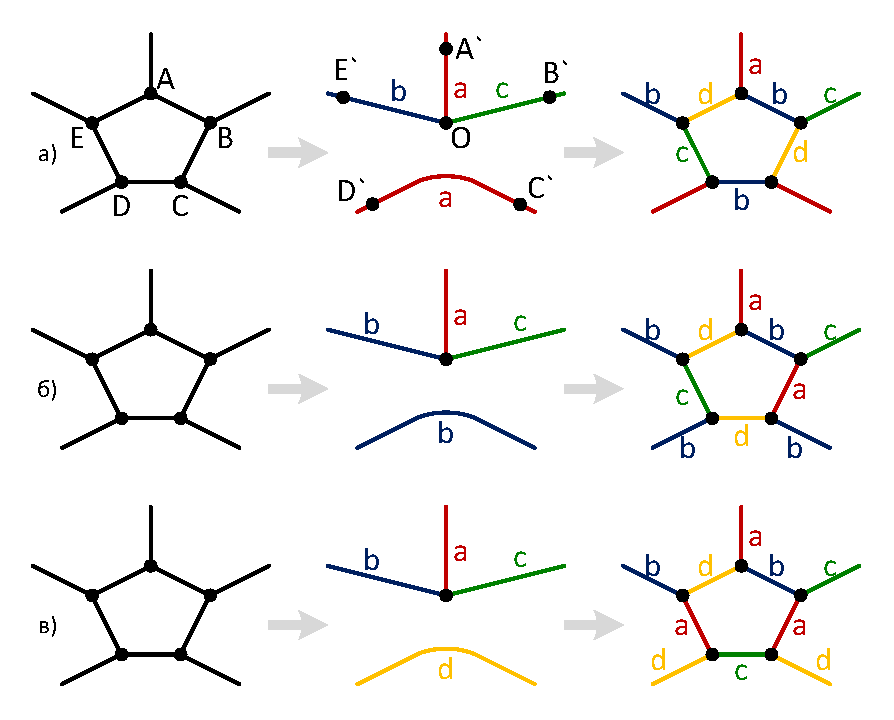
\includegraphics[width=1.0\textwidth]{fig/par_coloring4_face5.pdf}
\singlespacing
\captionstyle{center}\caption{Случай наличия в графе пятиугольной грани.}
\label{fig:text_3_graph_prim_coloring4_face5}
\end{figure}

Рассмотрим пятиугольную грань $ABCDE$.
Удалим ребра $ED$ и $BC$.
Стянем вершины $E$, $A$, $B$ в одну вершину $O$.
Стянем вершины $D$, $C$ в одну вершину степени 2, которую сразу удалим, соединим инцидентные ей ребра в одно $D'C'$ (см. рис.~\ref{fig:text_3_graph_prim_coloring4_face5}, а).
Так как в графе отсутствовали треугольные грани, то ни одна грань кроме $ABCDE$ не выродилась.
Таким образом, мы получили граф с $n - 4$ вершинами, ребра которого могут быть раскрашены в 4 цвета.
По этой раскраске построим раскраску исходного графа.
Для этого перенесем цвета всех ребер на исходный граф, непокрашенными останутся только ребра цикла $A-B-C-D-E$.
Если для покраски ребер $OA'$, $OE'$, $OB'$, $D'C'$ были использованы только три цвета ($a$, $b$, $c$), то без ограничения общности можно рассмотреть только два варианта раскраски: $\gamma(D'C') = \gamma(OA')$ (см. рис.~\ref{fig:text_3_graph_prim_coloring4_face5}, а) и $\gamma(D'C') \ne \gamma(OA')$ (см. рис.~\ref{fig:text_3_graph_prim_coloring4_face5}, б). 
Случай же, когда для покраски ребер $OA'$, $OE'$, $OB'$, $D'C'$ были использованы все 4 цвета, представлен на рис.~\ref{fig:text_3_graph_prim_coloring4_face5}, в.
Во всех трех случаях ребра цикла $A-B-C-D-E$ могут быть раскрашены с сохранением правильной реберной раскраски в 4 цвета.

Рассмотрев все возможные случаи нам удалось раскрасить текущий граф с $n$ вершинами в 4 цвета, опираясь на реберные раскраски графов меньших порядков.
Таким образом, предположение индукции верно, и плоский кубический граф может быть раскрашен в 4 цвета.

Доказательство существования раскраски конструктивно, алгоритм раскраски может быть построен путем стягивания гамаков и граней графа вплоть до графов минимального размера, с последующим восстановлением и посторением раскраски.
Каждое действие по стягиванию и построению раскраски текущего графа на основе раскраски графа меньшего порядка, осуществляется за количество действий $O(1)$.
Каждое стягивание уменьшает количество граней графа хотя бы на 1, таким образом общая сложность алгоритма $O(\zeta)$, что для кубического графа равносильно $O(\nu)$ или $O(\varepsilon)$.
$\blacksquare$\\

\subsubsection{Реберная раскраска в 3 цвета}

Утверждение о возможности раскраски ребер плоского кубического графа в три цвета является горазд более сильным, чем возможность раскраски в 5 и 4 цвета, оно верно для плоских кубических графов без мостов и равносильно задаче о четырех красках \cite{Soifer2009,Tait1880}.
Если кубический граф допускает правильную реберную раскраску в 3 цвета, то такая раскраска называется раскраской Тейта.
В цикле работ \cite{Kurapov2018,Kurapov2020,Kurapov2020Mono} авторы предлагают способ построения раскраски Тейта для плоских кубических графов, который мы будем использовать в этом разделе.
Кубический граф, порожденный односвязной поверхностной расчетной сеткой, является плоским и не содержит мостов, поэтому такой способ построения раскраски Тейта для него применим.

Рассмотрим принцип и реализацию алгоритма построения раскраски Тейта для кубического графа, являющегося дуальным графом для замкнутой поверхностной неструктурированной расчетной сетки.
В работах \cite{Kurapov2018,Kurapov2020} рассматривается подход к построению раскраски Тейта путем удаления ребер из исходного плоского кубического графа.
Ребра удаляются по тех пор, пока не будет получен кубический граф с уже известной раскраской.
После этого ребра возвращаются в граф в обратном порядке с соответствующей коррекцией раскраски.
Операцию удаления ребра из графа будем называть редуцированием кубического графа по ребру.
Для того чтобы редуцирование кубического графа по ребру можно было использовать для построения раскраски Тейта, необходимо уметь провести последовательность редукций до достижения простого по структуре кубического графа, раскраска которого не представляет сложности.
При этом, в получающихся графах допустимо наличие параллельных ребер, однако запрещено появление петель, так как раскраска Тейта для кубического графа с петлями невозможна.
Рассмотрим операцию редуцирования графа более подробно.

Сначала рассмотрим выполнение редуцирования кубического графа по ребру $e$ с концами $v_1$ и $v_2$, где инцидентными ребрами вершины v1 являются ребра $e$, $e_1(v_1)$, $e_2(v_1)$, а инцидентными ребрами вершины $v_2$ являются ребра $e$, $e_1(v_2)$, $e_2(v_2)$, а также среди ребер $e$, $e_1(v_1)$, $e_2(v_1)$, $e_1(v_2)$, $e_2(v_2)$ нет параллельных (см. рис.~\ref{fig:text_3_edge_coloring_1}, слева).
Из этого следует, что существует только одно ребро, соединяющее вершины $v_1$ и $v_2$.
В этом случае будем говорить, что редуцирование выполняется по уникальному ребру $e$.

\begin{figure}[ht]
\centering
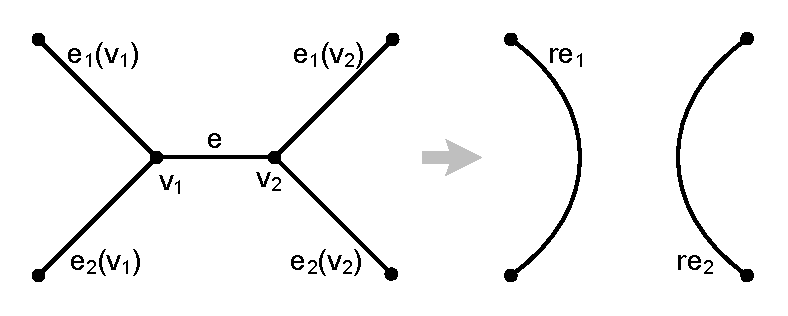
\includegraphics[width=0.8\textwidth]{fig/par_edge_col_1-pic-reduce-edge-type-1.pdf}
\singlespacing
\captionstyle{center}\caption{Редуцирование по уникальному ребру.}
\label{fig:text_3_edge_coloring_1}
\end{figure}

При выполнении редуцирования по ребру $e$ само ребро $e$ удаляется, также удаляются вершины $v_1$ и $v_2$, ребра $e_1(v_1)$ и $e_2(v_1)$ склеиваются в результирующее ребро $re_1$, ребра $e_1(v_2)$ и $e_2(v_2)$ склеиваются в ребро $re_2$ (см. рис.~\ref{fig:text_3_edge_coloring_1}, справа).

Другим случаем редуцирования является вариант, при котором также концами рассматриваемого ребра $e$ являются вершины $v_1$ и $v_2$, однако между ними проходит еще одно ребро, без ограничения общности будем считать, что это ребро $e_2(v_1) = e_2(v_2)$ (см. рис.~\ref{fig:text_3_edge_coloring_2}, слева).
В этом случае при редуцировании удаляется ребро $e$, удаляются вершины $v_1$ и $v_2$, а все три ребра $e_1(v_1)$, $e_2(v_1) = e_2(v_2)$, $e_1(v_2)$ склеиваются в единое ребро $re_1 = re_2$ (см. рис.~\ref{fig:text_3_edge_coloring_2}, справа).
Такой шаг редуцирования будем называть редуцированием по параллельному ребру.

\begin{figure}[ht]
\centering
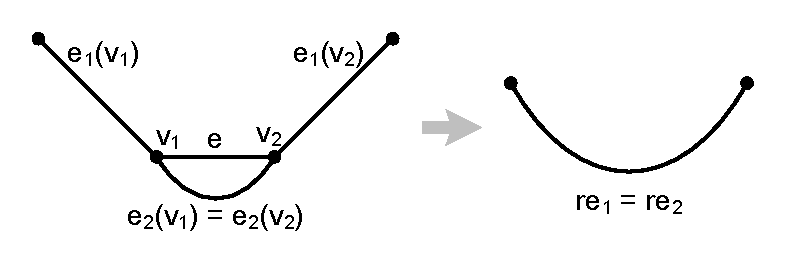
\includegraphics[width=0.8\textwidth]{fig/par_edge_col_2-pic-reduce-edge-type-2.pdf}
\singlespacing
\captionstyle{center}\caption{Редуцирование по параллельному ребру.}
\label{fig:text_3_edge_coloring_2}
\end{figure}

Отдельно отметим случай, когда между двумя вершинами проходит три параллельных ребра.
Если мы достигли такого графа, то это и есть минимальный кубический граф, построение раскраски для которого очевидно, и от которого нужно двигаться в обратную сторону, постепенно восстанавливая исходный граф.
Также следует рассмотреть случай, при котором после редуцирования по уникальному ребру граф перестает быть связным.
Это значит, что в исходном графе ребро $e$ было мостом, такие графы рассматривать не будем.
В других случаях в графе найдется либо уникальное, либо параллельное ребро, по которому можно осуществить следующий шаг редуцирования.

В качестве примера рассмотрим редуцирование графа, представляющего собой куб, как показано на рис.~\ref{fig:text_3_edge_coloring_3}.

\begin{figure}[ht]
\centering
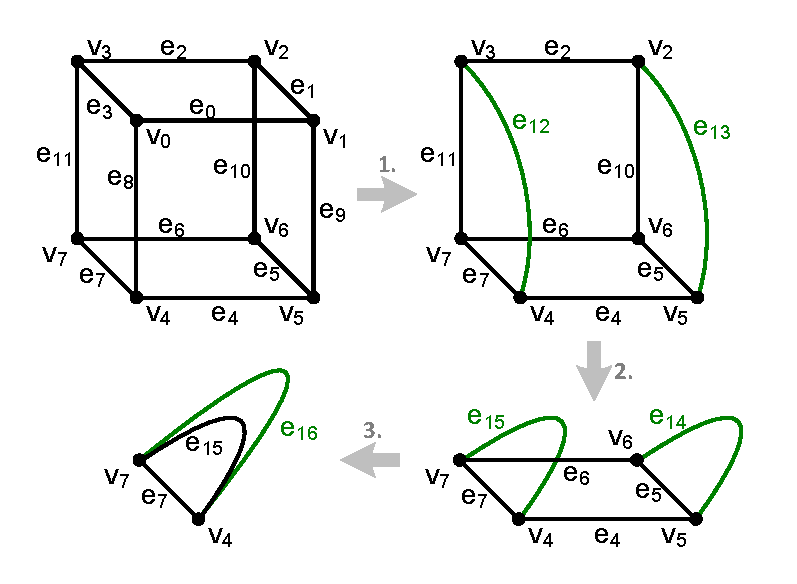
\includegraphics[width=0.8\textwidth]{fig/par_edge_col_3-reduce-0.pdf}
\singlespacing
\captionstyle{center}\caption{Полное редуцирование графа.}
\label{fig:text_3_edge_coloring_3}
\end{figure}

На рис.~\ref{fig:text_3_edge_coloring_3} представлен кубический граф, содержащий 8 вершин $v_0$ -- $v_7$ и 12 ребер $e_0$ -- $e_{11}$.
Будем считать, что нижние индексы в именах вершин и ребер являются также их идентификаторами.
Для полного редуцирования указанного графа требуется выполнение 3 шагов, которые могут быть записаны в историю редуцирования следующим образом:

$e_0 [(v_0 : e_3, e_8 \rightarrow e_{12}), (v_1 : e_1, e_9 \rightarrow e_{13})]$

$e_2 [(v_2 : e_{13}, e_{10} \rightarrow e_{14}), (v_3 : e_{12}, e_{11} \rightarrow e_{15})]$

$e_5 [(v_5 : e_4, e_{14} \rightarrow e_{16}), (v_6 : e_6, e_{14} \rightarrow e_{16})]$

По такой записи истории редуцирования можно идентифицировать каждый шаг, определить его тип (редуцирование по уникальному ребру или по параллельному) и выполнить восстановление графа.

Опираясь на указанные операции редуцирования можно описать алгоритм построения раскраски Тейта во время восстановления графа.

Прежде чем перейти к описанию алгоритма построения раскраски, рассмотрим центральный объект, который будет использован в этом построении.
Без ограничения общности будем считать, что раскраска выполняется в следующие цвета: красный, синий и зеленый, -- эти же цвета будем приводить на иллюстрациях.
Путь ребра некоторого кубического графа правильным образом раскрашены в три цвета.
Рассмотрим произвольные два цвета -- например, красный и синий.
Если рассмотреть все ребра, покрашенные в эти два цвета, а также все инцидентные им вершины, то получим граф порядка 2, у которого в каждой вершине сходятся разноцветные ребра.
Очевидно, такой граф является объединением простых циклов четной длины (двухцветных циклов).
На рис.~\ref{fig:text_3_edge_coloring_4} приведен пример такого двухцветного красно-синего цикла.

\begin{figure}[ht]
\centering
\includegraphics[width=0.6\textwidth]{fig/par_edge_col_4-bicolor-cycle.pdf}
\singlespacing
\captionstyle{center}\caption{Полная замена цветов в двухцветном цикле.}
\label{fig:text_3_edge_coloring_4}
\end{figure}

С таким двухцветным циклом можно выполнять следующие операции.
Во-первых, для всех ребер двухцветного цикла можно заменить цвет на противоположный, после чего раскраска в исходном графе останется правильной (см. рис.~\ref{fig:text_3_edge_coloring_4}).
Также можно применить перекраску в противоположный цвет не всех ребер цикла, а только расположенных между двумя фиксированными ребрами $e_1$ и $e_2$ (на рис.~\ref{fig:text_3_edge_coloring_5} приведены два варианта такой перекраски в порядке обхода цикла по часовой и против часовой стрелки).
При такой перекраске ребер в цикле возникает два конфликта по цветам: между ребрами $e_1$ и $e_2$ и их перекрашенными соседями.

\begin{figure}[ht]
\centering
\includegraphics[width=0.8\textwidth]{fig/par_edge_col_5-bicolor-cycle-partial-switch.pdf}
\singlespacing
\captionstyle{center}\caption{Частичная замена цветов в двухцветном цикле.}
\label{fig:text_3_edge_coloring_5}
\end{figure}

Смысл частичной замены цветов в двухцветном цикле становится понятным, если возникает необходимость поместить в граф новое ребро.
На рис.~\ref{fig:text_3_edge_coloring_6} продемонстрирована операция, при которой выполняется частичная перекраска цикла между ребрами $e_1$ и $e_2$, а затем на ребра $e_1$ и $e_2$ добавляются новые вершины $v_1$ и $v_2$ соответственно, между которыми проводится ребро.
В завершение полученные после разбиения ребер $e_1$ и $e_2$ более мелкие ребра перекрашиваются для устранения конфликтов.
Новое проведенное ребро при этом перекрашивается в третий свободный цвет, что приводит к сохранению правильной раскраски во всем графе.
Таким образом, выбрав два произвольных ребра на любом двухцветном цикле, мы можем добавить новое ребро с концами на выбранных ребрах, а затем перекрасить ребра и сохранить правильную реберную раскраску.
Такую операцию будем называть восстановлением ребра по двухцветному циклу.

\begin{figure}[ht]
\centering
\includegraphics[width=0.8\textwidth]{fig/par_edge_col_6-bicolor-cycle-new-edge.pdf}
\singlespacing
\captionstyle{center}\caption{Замена цветов в двухцветном цикле при добавлении нового ребра.}
\label{fig:text_3_edge_coloring_6}
\end{figure}

Также нам понадобится операция поиска двухцветного цикла, начиная с произвольного ребра $e$, и содержащего ребра цветов $\gamma(e)$ и $c \ne \gamma(e)$. Такой цикл всегда существует и он ровно один.

Теперь, имея в своем распоряжении три простые операции: поиск двухцветного цикла по ребру и второму цвету, перекраска двухцветного цикла и восстановление ребра по двухцветному циклу, -- мы можем описать алгоритм восстановления одного шага редуцирования графа с сохранением правильной реберной раскраски (см. рис.~\ref{fig:text_3_edge_coloring_7}).

Дополнительно отметим, что восстановление шага редуцирования графа по параллельному ребру не представляет сложности, так как это локальная операция, которая затрагивает единственное результирующее ребро. Поэтому рассмотрим подробно только восстановление шага редуцирования по уникальному ребру.

Пусть мы имеем шаг редуцирования графа, результирующими ребрами после выполнения которого являются различные ребра $re_1$ и $re_2$.
В процессе восстановления мы должны поместить на эти ребра новые вершины $v_1$ и $v_2$ соответственно, провести между ними ребро и выполнить коррекцию раскраски.
Опишем последовательность действий в этом случае.

Вариант 1. Если результирующие ребра $re_1$ и $re_2$ имеют разные цвета, то найдем двухцветный цикл, начиная с ребра $re_1$, включающий в себя ребра цветов $\gamma(re_1)$ и $\gamma(re_2)$.
Если найденный цикл содержит также и ребро $re_2$, то можно выполнить восстановление исходного ребра по найденному двухцветному циклу.
В противном случае перекрасим найденный двухцветный цикл.
Так как перекрашивание затронет только ребро $re_1$, то после этой операции мы получим ситуацию, в которой ребра $re_1$ и $re_2$ имеют один цвет. В этом случае переходим ко второму варианту.

\begin{figure}[ht]
\centering
\includegraphics[width=1.0\textwidth]{fig/par_edge_col_7-algorithm.pdf}
\singlespacing
\captionstyle{center}\caption{Итерация алгоритма восстановления и перекраски графа.}
\label{fig:text_3_edge_coloring_7}
\end{figure}

Вариант 2. Если результирующие ребра $re_1$ и $re_2$ имеют один и тот же цвет, то рассмотрим два оставшихся цвета: $x$ и $y$.
Рассмотрим два двухцветных цикла, начиная с ребра $re_1$.
Причем в первый цикл будем включать ребра с цветами $\gamma(re_1)$ и $x$, а во второй цикл будем включать ребра с цветами $\gamma(re_1)$ и $y$.
Если один из найденных двухцветных циклов будет содержать также и ребро $re_2$, то по этому циклу и нужно выполнить восстановление исходного ребра, которое было удалено из графа при редуцировании.
Вопрос содержания ребра $re_2$ в одном из двухцветных циклов $\gamma(re_1) - x$ и $\gamma(re_1) - y$ оставим без доказательства (его можно найти в \cite{Kurapov2018}).

\begin{figure}[ht]
\centering
\includegraphics[width=0.8\textwidth]{fig/par_edge_col_8-restore-and-repaint.pdf}
\singlespacing
\captionstyle{center}\caption{Восстановление и раскраска графа.}
\label{fig:text_3_edge_coloring_8}
\end{figure}

На рис.~\ref{fig:text_3_edge_coloring_8} приведена последовательность восстановления графа, редуцирование которого продемонстрировано на рис.~\ref{fig:text_3_edge_coloring_3}.
Приведем еще раз историю редуцирования графа:

$e_0 [(v_0 : e_3, e_8 \rightarrow e_{12}), (v_1 : e_1, e_9 \rightarrow e_{13})]$

$e_2 [(v_2 : e_{13}, e_{10} \rightarrow e_{14}), (v_3 : e_{12}, e_{11} \rightarrow e_{15})]$

$e_5 [(v_5 : e_4, e_{14} \rightarrow e_{16}), (v_6 : e_6, e_{14} \rightarrow e_{16})]$

Первый шаг восстановления относится к редуцированию по параллельному ребру.
Ребро $e_{16}$ разбивается на три ребра $e_6$, $e_{14}$, $e_4$ с помощью вершин $v_6$ и $v_5$.
Между вершинами $v_6$ и $v_5$ восстанавливается ребро $e_5$.
Ребра $e_6$ и $e_4$ наследуют зеленый цвет ребра $e_{16}$, а ребра $e_{14}$ и $e_5$ раскрашиваются в два оставшиеся цвета.

Второй шаг восстановления относится к редуцированию по уникальному ребру.
Сначала ищется красно-синий цикл, содержащий ребро $e_{14}$.
Так как он не содержит ребро $e_{15}$, то цикл из двух ребер $e_{14}-e_5$ перекрашивается.
После этого ищется сине-зеленый цикл, содержащий ребро $e_{14}$.
Это цикл $e_{14}-e_6-e_{15}-e_4$, и он содержит ребро $e_{15}$.
Происходит восстановление ребра по найденному двухцветному циклу.

Третий шаг восстановления также относится к редуцированию по уникальному ребру.
Так как существует сине-красный цикл $e_{12}-e_2-e_{13}-e_5-e_6-e_7$, то сразу можно выполнить восстановление ребра по этому циклу (а в этом случае можно выполнить восстановление и по сине-зеленому циклу, что приведет к другой раскраске).

Очевидно, что алгоритм имеет квадратичную сложность по порядку графа, так как количество шагов восстановления пропорционально порядку исходного графа, а на каждом шаге восстановления уникального ребра необходимо выполнять поиск и перекраску двухцветных циклов, что в худшем случае пропорционально порядку текущего графа.

Если мы рассматриваем кубический граф порядка $n$, то он содержит $\frac{3n}{2}$ ребер, причем $n$ четно.
Если этот граф допускает правильную реберную раскраску в 3 цвета, то в каждый из цветов раскрашено ровно $\frac{n}{2}$ ребер.
Таким образом, множество ребер распадается на 3 одинаковых по размеру подмножеств ребер без конфликтов.
Вызывает интерес вопрос о процентном соотношении ребер, раскрашенных в разные цвета, для жадной раскраски в 5 цветов при порядке графа, стремящемся к бесконечности.

\begin{figure}[ht]
\centering
\includegraphics[width=0.8\textwidth]{fig/par_edge_col_9-bubble.pdf}
\singlespacing
\captionstyle{center}\caption{Генерация кубического графа.}
\label{fig:text_3_edge_coloring_9}
\end{figure}

Для экспериментального получения такого распределения будем строить искусственные кубические графы следующим образом.
В качестве нулевого графа возьмем кубический граф $K_4$, далее последовательно в текущем кубическом графе будем случайным образом выбирать вершину и заменять ее на треугольную конструкцию, как показано на рис.~\ref{fig:text_3_edge_coloring_9}.
Вполне очевидно, что получающиеся таким образом графы будут кубические, и что они допускают правильную реберную раскраску в три цвета.
К полученным сгенерированным кубическим графам порядка более $10^5$ был применен жадный линейный алгоритм реберной раскраски в 5 цветов.
Получившееся распределение цветов представлено на рис.~\ref{fig:text_3_edge_coloring_10}.

\begin{figure}[ht]
\centering
\includegraphics[width=0.6\textwidth]{fig/par_edge_col_10-chart.png}
\singlespacing
\captionstyle{center}\caption{Распределение процентной доли цветов для разных раскрасок.}
\label{fig:text_3_edge_coloring_10}
\end{figure}

Из рис.~\ref{fig:text_3_edge_coloring_10} видно, что распределение цветов жадной раскраски устроено примерно следующим образом.
Большинство ребер кубического графа практически равномерно раскрасилось в 3 цвета, однако для окрашивания около 10\% ребер потребовалось использование четвертого цвета, а для окрашивания около 1,5\% ребер пришлось задействовать пятый цвет.

Для оценки целесообразности применения реберной раскраски для устранения конфликтов по данным при расчете потоков в задаче моделирования процесса обледенения поверхности были выполнены запуски модельной задачи на одном вычислительном узле на базе микропроцессора Intel Xeon Phi 7290 KNL\label{abbr:knl-3}.
Этот микропроцессор имеет 72 ядра, на каждом из которых может быть запущено до 4 потоков.
Таким образом, на этом микропроцессоре возможно распараллеливание запуска на 288 потоков.

Для сравнения эффективности методов устранения конфликтов при параллельном расчете потоков через границы ячеек замерялось ускорение вычислений при распараллеливании $s_{shr}$ эффективность распараллеливания $e_{shr}$.
Сравнивались два метода устранения конфликтов по доступу к данным: использование \texttt{omp atomic} операций и разделение множества ребер на неконфликтующие подмножества с помощью реберной раскраски.

\begin{figure}[ht]
\centering
\includegraphics[width=1.0\textwidth]{fig/par_edge_col_11-chart.png}
\singlespacing
\captionstyle{center}\caption{Эффективность распараллеливания пересчета потоков для разных способов устранения конфликтов по данным.}
\label{fig:text_3_edge_coloring_11}
\end{figure}

Из рис.~\ref{fig:text_3_edge_coloring_11} можно заметить, что при использовании распараллеливания на относительно небольшое количество потоков нет существенной разницы между рассмотренными методами устранения конфликтов.
Однако при возрастании количества используемых потоков метод реберной раскраски становится гораздо эффективнее, чем использование директивы \texttt{omp atomic} с точки зрения эффективности распараллеливания.

\subsubsection{Исследование масштабируемости плотных векторизованных вычислений}

В этом разделе приводится эксперимент, который был поставлен для анализа масштабируемости высокопроизводительных вычислений на общей памяти на разных узлах суперкомпьютера МВС-10П.
В рамках этого эксперимента был взят один и тот же расчетный код, но в двух реализациях -- скалярная реализация без использования векторных инструкций и векторная реализация.

В качестве анализируемого кода выбрано численное решение задачи газовой динамики методом Годунова с использованием точного римановского решателя.
Точный римановский решатель является численным решением задачи Римана о распаде произвольного разрыва (в которой требуется определить состояние газа на границе двух сред в момент устранения перегородки, разделяющей два объема газа с разным состоянием).
Реализация точного римановского решателя \cite{riemannvecGithub} представлена функцией \texttt{solver}, принимающая на вход наборы газодинамических параметров слева и справа от перегородки, и выдающая значения газодинамических параметров в месте разрыва в момент устранения перегородки.
Была использована векторизованная версия точного римановского решателя \texttt{solver\_16}, в которой за один вызов функции \texttt{solver\_16} решается 16 экземпляров задачи о распаде разрыва (векторизуется 16 вызовов функции \texttt{solver}).
Таким образом, эксперимент ставился с целью сравнить эффективность распараллеливания на общей памяти скалярного кода и аналогичного ему плотного веторизованного кода \cite{Vorobyov2020ParVec,Vorobyov2020Scaling}.

Проводились тестовые запуски на всех типах вычислительных узлов суперкомпьютера МВС-10П: Haswell, Broadwell, KNL\label{abbr:knl-4}, Skylake, Cascade Lake (характеристики узлов приведены в таблице~\ref{tbl:text_2_scaling_supercomputers}).

На рис.~\ref{fig:text_3_omp2} сверху слева представлены графики ускорения скалярной версии римановского решателя при увеличении количества потоков с 1 до 160.
Для каждого вычислительного узла явно просматриваются отрезки квазилинейного ускорения, которые завершаются заметными провалами.
Длина этих отрезков во всех случаях равняется суммарному количеству ядер в узле, а провалы обусловлены конфликтами за аппаратные ресурсы.
При этом стоит отметить, что хоть максимальное количество доступных потоков для вычислительного узла на базе микропроцессора KNL равняется 288, однако на графике не показаны значения больше 160, так как сверх этого значения наблюдается только деградация производительности, и наиболее эффективное использование зафиксировано в районе 140 потоков.
Также можно отметить, что для всех микропроцессоров ускорение близко к линейному до тех пор, пока каждый поток запущен на своем отдельном ядре.

\begin{figure}[ht]
\centering
\includegraphics[width=1.0\textwidth]{./fig/par_openmp_scalar_vec_chart_big.png}
\singlespacing
\caption{Графики ускорения и эффективности распараллеливания скалярных и векторизованных вычислений.}
\label{fig:text_3_omp2}
\end{figure}

На рис.~\ref{fig:text_3_omp2} слева представлены графики ускорения скалярной и векторной версии газодинамического решателя на 1-160 потоках.
Для каждого вычислительного узла явно просматриваются отрезки квазилинейного ускорения, которые завершаются провалами.
Длина этих отрезков совпадает с количеством ядер в узле, а провалы обусловлены конкуренцией за аппаратные ресурсы.
Для всех узлов ускорение близко к линейному до тех пор, пока каждый поток запущен на своем ядре.
Из графиков эффективности распараллеливания видно, что эффективность распараллеливания векторных версий кода примерно вдвое ниже эффективности распараллеливания скалярных версий.
Это говорит о целесообразности векторизации программного кода при достижении ускорения от векторизации хотя бы в два раза.

%---------------------------------------------------------------------------------------------------

\subsection{Выводы из главы}

Разработана архитектура блочно-структурированной расчетной сетки с поддержкой дробления блоков.
Рассмотрены алгоритмы распределения блоков расчетной сетки между вычислительными процессами без дробления блоков: алгоритм с экспоненциальной сложностью для нахождения точного решения и приближенный жадный алгоритм.
Из сравнения алгоритмов распределения без дробления блоков сделан вывод о необходимости разработки алгоритмов с дроблением.

Предложены различные алгоримты распределения блоков расчетной сетки по вычислительным процессам с дроблением блоков.
Рассмотрен алгоритм, обеспечивающий наилучший показатель неравномерности распределения $D$, но допускающий большое количество дроблений блоков и порождающий блоки с малыми размерами, применение этого алгоритма признано нецелесообразным из-за высокой вычислительной сложности.
Рассмотрен приближенный алгоритм распределения с дроблениями блоков, основанный на жадном алгоритме распределения и дроблении пополам наиболее крупного блока до достижения требуемого значения показателя $D$, поставлен численный эксперимент по применению этого алгоритма.
Результаты алгоритма показали, что использование алгоритма распределения с дроблением крупных блоков пополам и низкого показателя неравномерности распределения $D$ приводит к резкому возрастанию количества дроблений и деградации производительности, из чего сделан вывод о необходимости разработки алгоритмов с уменьшение количества дроблений.
Рассмотрена группа алгоритмов с уменьшением количества дроблений и ограничениями на размеры блоков, основанных на рассмотрении всех возможных допустимых разрезов блоков.
Проведено сравнение этих алгоритмов на наборе случайных данных на основе количества разрезов и значения показателя $D$.

Рассмотрены различные алгоритмы декомпозиции поверхностной неструктурированной расчетной сетки.
При использовании алгоритмов декомпозиции, при которых значение $D$ достаточно мало, наблюдается возможность появления протяженных границ между доменами.
Предложен алгоритм сглаживания границ между доменами при декомпозиции поверхностной неструктурированной расчетной сетки позволяющий найти точное решение, снизив длины границ примерно на 10\%.
Поставлен численный эксперимент по масштабированию вычислений на поверхностной неструктурированной расчетной сетке с использованием декомпозиции с помощью иерархического деления доменов пополам и сглаживания границ между доменами, демонстирующий эффективность распараллеливания вычислений в районе 0,8 на сегментам суперкомпьютера МВС-10П на базе микропроцессоров Intel при использовании 1-64 вычислительных узлов.

Рассмотрены способы избавления от конфликтов по данным при решении задачи моделирования обледенения и распараллеливании вычислений на общей памяти.
Для избавления от конфликтов по данным с помощью реберной раскраски дуального графа расчетной сетки рассмотрены алгоритмы реберной раскраски плоского кубического графа без мостов в 5, 4 и 3 цвета, использование этих алгоритмов приводит к ускорению вычислений при большом количестве параллельных потоков по сравнению с использованием директив OpenMP.

Поставлен эксперимент по исследованию распаралллеливания расчетных кодов на общей памяти на сегментах суперкомпьютера МВС-10П на базе микропроцессоров Intel.
Проведено сравнение распараллеливания скалярного расчетного кода и аналогичного ему векторного кода из чего сделан вывод, что распараллеливание векторного кода на общей памяти примерно вдвое менее эффективно, чем скалярного.
Сделан вывод, что векторизация расчетных кодов имеет смысл при достижении хотя бы двукратного ускорения.

%---------------------------------------------------------------------------------------------------
